% !TeX spellcheck = pl-PL
%\cleardoublepage
%\phantomsection
\chapter{Przegląd metod śledzenia ruchu}\label{chap:literature}

Śledzenie ruchu ma zastosowanie zarówno w~przypadku istot żywych (ludzie i~zwierzęta), jak i~w~przypadku obiektów nieożywionych. W~zależności od budowy śledzonego obiektu można stosować różne techniki i~narzędzia. Za pomocą innych technik będzie śledzony ruch człowieka, który charakteryzuje się specyficzną dla ludzi kinematyką i~dynamiką zmian ułożenia ciała, a~inaczej będzie śledzony fizyczny przedmiot, który z~jednej strony może podlegać fizycznie ograniczonemu ruchowi (np.: ruch wystrzelonego pocisku w~polu grawitacyjnym), a~z drugiej strony może być immanentnie wyposażony w~pomocnicze, autonomiczne urządzenia pomiarowe (np.: rakieta wyposażona w~GPS, akcelerometr i~żyroskop). 

W doborze techniki śledzenia ruchu istotną rolę odgrywa także określenie celu oraz pożądanej dokładności procesu śledzenia. Jeśli przykładowo celem jest określenie położenia poszczególnych stawów ludzkiego ciała, wówczas niezbędne będzie zastosowanie systemów śledzenia ruchu postaci, które gwarantują dużą dokładność szacowania pozycji stawów. Jeśli istotne jest tylko zgrubne określenie położenia całej postaci w~jej otoczeniu, wówczas wystarczy przykładowo wykorzystanie systemu pozycjonowania GPS, przyczepionego do korpusu śledzonej osoby.

Innym istotnym aspektem, który determinuje zastosowanie techniki śledzenia ruchu, jest wykorzystanie konkretnych (dostępnych) urządzeń pomiarowych. Charakterystyka urządzeń pomiarowych wpływa na dobór metod analizy danych zwracanych przez urządzenia pomiarowe i~końcową dokładność śledzenia zmian obiektu. Istotnym czynnikiem wpływającym na konstrukcję i~oprogramowanie systemu śledzenia jest przewidywany zakres prędkości wykonywanego ruchu, który musi zostać zarejestrowany i~zinterpretowany przez system pomiarowy. Przykładem ruchów człowieka o~skrajnie różnej dynamice  mogą być ćwiczenia rehabilitacyjne kończyn po urazach oraz dynamika ręki tenisisty podczas serwisu.  

W literaturze przedmiotu można znaleźć wiele opisów prowadzonych prac badawczych, które bazując na charakterystyce śledzonego obiektu lub dostępnych urządzeniach pomiarowych próbując pokonać trudności związane z~niedostateczną dokładnością śledzenia ruchu, bądź niedostateczną czułością i~bezwładnością układu pomiarowego w~przypadku dużych prędkości zmian śledzonego obiektu. Istnieje też szereg prac, które stosując heterogeniczne systemy śledzenia, kompensują niedoskonałości składowych układów śledzących. 
Przegląd wybranych publikacji, sprofilowany głównie na śledzenie ruchu postaci ludzkiej, został przedstawiony w~kolejnych podrozdziałach.

\section{Systemy śledzenia ruchu postaci} \label{sec:literature:mocapSystems}

Śledzenie ruchu postaci jest procesem obliczeniowym mającym na celu jednoznaczne określenie w~czasie i~w~przestrzeni położenia i~orientacji układu punktów (stawów) opisujących pozy człowieka. 

Jednym z~kryterium podziału systemów śledzenia ruchu człowieka jest jego zastosowanie. Głównymi obszarami zastosowań dyskutowanych systemów śledzenia są: nadzór, kontrola oraz analiza ruchu ludzkiego ciała \cite{Moeslund2001}. Pod pojęciem nadzoru rozumiemy systemy śledzące zachowanie człowieka i~na jego podstawie oceniające np. czy dana osoba potrzebuje pomocy \cite{Kwolek, Kepski2016, Haritaoglu}. Obszar zastosowań związanych z~kontrolą odnosi się do interakcji człowiek--komputer np.: w~grach komputerowych, środowiskach wirtualnych, czy animacji \cite{Moeslund2001a}. Ostatni z~wymienionych obszarów zastosowań - analiza, obejmuje takie zagadnienia jak diagnostyka i~rehabilitacja medyczna \footfullcite{footnote:Even-zohar1984} \footfullcite{footnote:XsensRehab}, czy wspomaganie treningu sportowego\footfullcite{footnote:inmotio} \cite{Neville2010,Noiumkar2013}.

Innym kryterium podziału systemów śledzenia ruchu człowieka jest zastosowana w~nich technologia, pozwalająca obserwować śledzoną osobę. Systematykę tę przedstawia diagram przedstawiony na rysunku \ref{fig:literature:mocapSystems:diagram}. Kolejne części niniejszego rozdziału zostały poświęcone przybliżeniu istotnych cech każdego z~systemów śledzenia ruchu przedstawionych na wspomnianym wcześniej diagramie.

%Spośród wymienionych technologii w~obszarze zainteresowań pozostaną jedynie systemy optyczne, którym poświęcone zostaną kolejne podrozdziały. W~zakresie zastosowań dalsze rozważania będą najbliższe systemom analitycznym z~dużym potencjałem w~zakresie kontroli ruchu postaci.

\subsection{Optyczne systemy śledzenia ruchu}
Optyczny system śledzenia ruchu to system, który dane o~ruchu obiektu pozyskuje się za pośrednictwem toru optycznego uzbrojonego w~czujniki optyczne (np. kamer video, sensorów podczerwieni i~in.). Jeśli informacje o~ruchu można pozyskać na podstawie zbioru kontrolowanych punktów (markerów) identyfikujących śledzony obiekt to takie systemy nazywamy systemami śledzenia wykorzystującymi markery (ang. \textsl{marker-based tracking system}). Przykładem tego typu systemów śledzenia ruchu mogą być produkty firm Vicon \footfullcite{footnote:ViconWebsite}, Qualisys \footfullcite{footnote:QulisysWebsite}, czy Optitrack \footfullcite{footnote:OptitrackWebsite}. Istnieją również systemy bezmarkerowe (ang. \textsl{markerless tracking system}), które fizyczne markery umieszczane na śledzonym obiekcie, zastępują punktami wyznaczanymi na podstawie cech charakterystycznych danych obiektów (na przykład dla ciała ludzkiego mogą to być punkty reprezentujące stawy). W takim przypadku, strumień danych otrzymany z czujników zostaje poddany analizie i przetwrzaniu w celu wyznaczenia punktów, które pozwalają śledzić ruch obiektu. Przykładami bezmarkerowych optycznych systemó śledzenia ruchu moga być komercyjny system śledzenia ruchu firmy Organic Motion \footfullcite{footnote:OrganicmoitonWebsite}, czy systemy tworzone na uniwersytetach Stanforda \footfullcite{footnote:StanfordBiomotion} i~Maryland \cite{Sundaresan2005,Sundaresan2007}.

Optyczne systemy śledzenia ruchu zbudowane są zazwyczaj z~dwóch rodzajów urządzeń. Pierwszym z~nich jest jedno lub wiele źródeł światła np.: kierunkowego, odbitego czy ustrukturyzowanego, a~drugim jest jeden, lub wiele czujników optycznych (kamer). Najpopularniejszymi systemami optycznymi wykorzystywanymi do śledzenia ruchu człowieka są te oparte o~analizę obrazów rejestrowanych przez jedną \cite{schmidt2006kernel,RuiLi2006} lub układ wielu kamer\footfullcite{footnote:ViconWebsite} \footfullcite{footnote:QulisysWebsite} \cite{Sundaresan2005,Krzeszowski2013}.

Przełomowym momentem dla rozwoju technik śledzenia ruchu postaciz~wykorzystaniem kamer był eksperyment przeprowadzony przez szwedzkiego psychologa Gunnara Johanssona, w~roku 1973, mający na celu zbadanie trajektorii ruchu kończyn człowieka poprzez umieszczenie na nich małych odblaskowych elementów, a~następnie filmowanie ich i~analizowanie zarejestrowanej trajektorii ruchu punktów odblaskowych. Eksperyment ten nazwany \emph{Moving Light Display} (\textbf{MLD}) \cite{Johansson1973} stał się wzorem dla budowania systemów śledzenia ruchu opartego o~kamery i~wykorzystującego markery umieszczone na ciele człowieka. Warto zaznaczyć, że główne założenia budowy ówczesnego systemu śledzenia ruchu wykorzystywane są również we współczesnych systemach śledzenia ruchu wykorzystujących kamery oraz markery.

\subsubsection*{Optyczne systemy śledzenia ruchu wykorzystujące markery}
Z punktu widzenia analizy optycznych systemów śledzenia ruchu wykorzystujących markery najistotniejszą cechą rozróżniającą stosowane markery jest to czy są one emiterem światła, czy jedynie je odbijają. Jeśli mamy do czynienia z~markerami będącymi równocześnie źródłem światła wówczas nazywamy je markerami aktywnymi, natomiast markery odbijające światło z~zewnętrznego źródła są nazywane markerami pasywnymi.

Markery pasywne, wykorzystywane w~optycznych systemach śledzenia ruchu, mogą różnić się swoim kształtem, wielkością, czy budową, w~zależności od ich przeznaczenia i~oczekiwanej dokładności. Różnice w~wielkości markerów można prześledzić na przykładzie markerów pasywnych, które wykorzystywane do śledzenia mimiki twarzy (problem wymagający dużej precyzji) mają średnicę od ok. 3 do ok. 5 mm, natomiast gdy mają być wykorzystywane do śledzenia położenia całej sylwetki (problem wymagający mniejszej precyzji lecz rejestracji markera z większej odległości) ich średnica wynosi zazwyczaj około 25mm \footfullcite{footnote:ViconMarkersSet}. Systemy śledzenia ruchu oparte o~markery pasywne opierają się dokładnie na pomyśle zaproponowanym przez G. Johanssona we wspomnianym wcześniej eksperymencie \textsl{MLD}. Jako współczesne realizacje optycznych systemów śledzenia ruchu stosujących markery pasywne można wymienić wspomniane już wielokamerowe profesjonalne systemy śledzenia firm Vicon, Qualisys, czy OptiTrack. 
Zamieszczony w~dalszej części pracy opis budowy i~zasad działania optycznego systemu śledzenia ruchu z~pasywnymi markerami zostanie przedstawiony na podstawie systemu firmy Vicon\footnote{Wybór ten został podyktowany dostępem do takowego systemu w~Centrum Technologii Informatycznych Politechniki Łódzkiej.} zainstalowanego na Politechnice Łódzkiej. 
Analizowany system firmy Vicon jest systemem wielokamerowym, który wykorzystuje wyspecjalizowane kamery cyfrowe video, o~wysokiej rozdzielczości matrycy (4 MPix dla rozważanego systemu), wyposażone w~filtr przepuszczający zakres światła podczerwonego. Każda z~kamer wyposażona jest równocześnie w~kierunkowe źródło światła emitujące fale z~zakresu światła podczerwonego. System Vicon dostępny na Politechnice Łódzkiej zbudowany jest z~10 takich kamer umieszczonych dookoła pomieszczenia laboratoryjnego tak jak jest to pokazane na rysunku \ref{fig:literature:vicon:lutSetup}, gdzie elementy oznaczone IR1..10 to kamery wyposażone w~filtr podczerwony, RGB1 i~RGB2 to dwie kamery video pozwalające rejestrować tradycyjny obraz kolorowy oraz stanowisko komputerowe oznaczone jako PC. System posiada swoją funkcjonalność w~tzw. przestrzeni roboczej śledzenia (ang. \textsl{tracking volume}). Jest to przestrzeń wyznaczona przez bryły widzenia kamer. Technicznie każdy marker w~przestrzeni roboczej powinien być widoczny jednocześnie przez 3 kamery, aby możliwe było precyzyjne określenie jego pozycji. Ruchy wykonywane poza przestrzenią roboczą nie są śledzone przez system lub obarczone są błędnymi wynikami.

\begin{savenotes}
							
	\begin{figure}[!htb]
		\centering	
		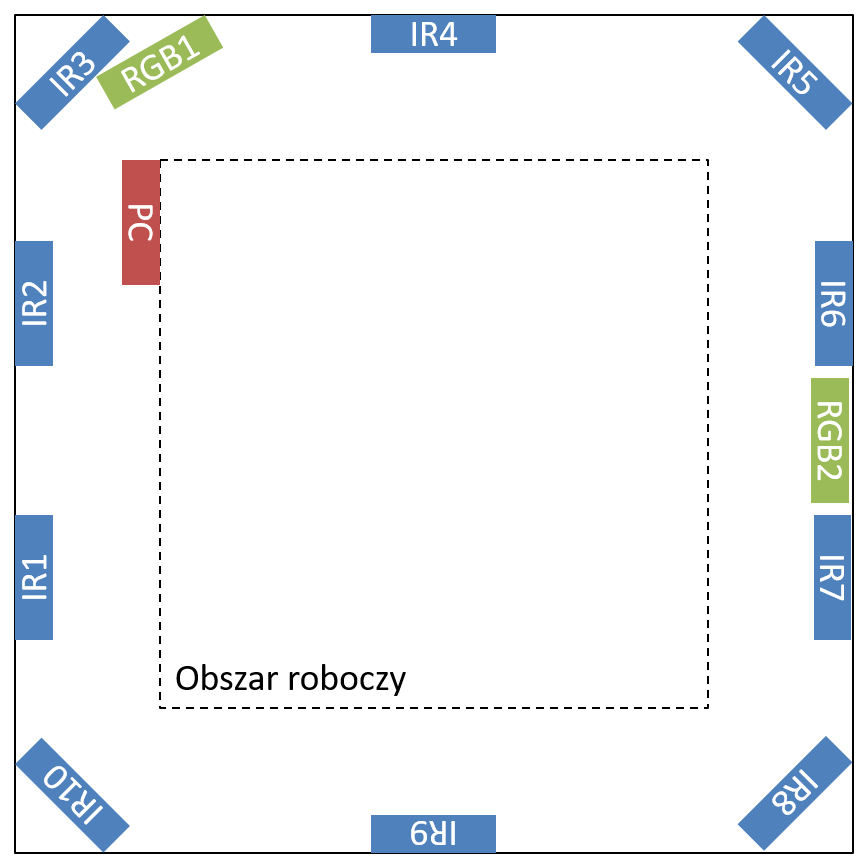
\includegraphics[width=0.75\textwidth]{images/viconSetup.png}
		\caption{Rysunek przedstawiający konfigurację sprzętową systemu Vicon dostępnego na Politechnice Łódzkiej. IR1..10 -- kamery z filtrem podczerwonym, RGB1, RGB2 -- kamery rejestrujący obraz kolorowy, PC -- stanowisko komputerowe ze specjalistycznym oprogramowaniem do obsługi systemu śledzenia.}
		\label{fig:literature:vicon:lutSetup}
	\end{figure}
						
\end{savenotes}
	
Kamery wykorzystane w~systemie Vicon posiadają filtr przepuszczający jedynie fale z~zakresu światła podczerwonego, co pozwala na stosunkowo łatwe wyodrębnienie z~rejestrowanego obrazu markerów odbijających światło podczerwone. Markery są elementami pokrytymi farbą odbijającą padające na nie światło w~kierunku źródła emisji promieni. Ponieważ w~przypadku zastosowanych kamer źródło światła jest umieszczone tuż obok obiektywu, oświetlone markery stanowią najjaśniejsze punkty na rejestrowanym obrazie. Na rysunku \ref{fig:literature:qualisys:markers} zaprezentowany został przykładowy zestaw markerów wykorzystywanych w~omawianym systemie śledzenia ruchu, natomiast na rysunku \ref{fig:literature:vicon:markers} widać aktora w~kombinezonie, przy którym owe markery są przymocowane. Markery wykorzystywane są do oznaczenia części ciała człowieka, których ruch będzie śledzony.
	
\begin{savenotes}
							
	\begin{figure}[!htb]
		\centering	
		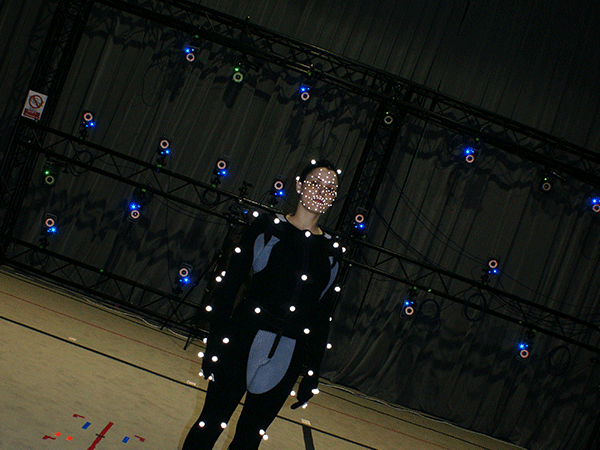
\includegraphics[width=0.65\textwidth]{images/markers-suits-600x450.png}
		\caption[Zestaw znaczników pasywnych w~systemie Vicon umieszczonych na ciele aktora w~trakcie sesji śledzenia ruchu]{Zestaw znaczników pasywnych w~systemie Vicon umieszczonych na ciele aktora w~trakcie sesji śledzenia ruchu \footfullcite{footnote:ViconMarkersSet}}
		\label{fig:literature:vicon:markers}
	\end{figure}
						
\end{savenotes}
		
\begin{savenotes}
							
	\begin{figure}[!htb]
		\centering	
		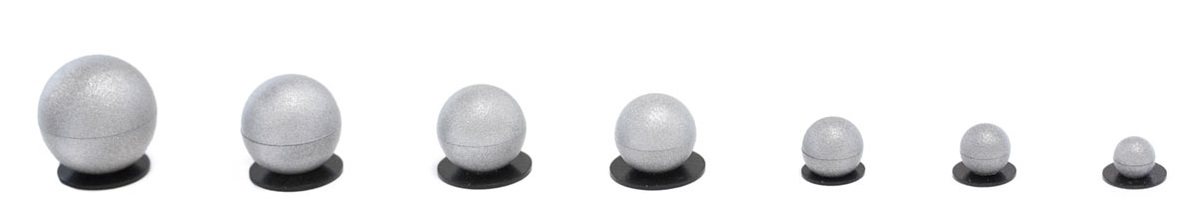
\includegraphics[width=0.65\textwidth]{images/super-spherical-markers-hero.jpg}
		\caption[Pasywne markery wykorzystywane w~optycznych systemach śledzenia ruchu]{Pasywne markery wykorzystywane w~optycznych systemach śledzenia ruchu\footfullcite{footnote:QulisysMarkers}}		
		\label{fig:literature:qualisys:markers}
	\end{figure}
						
\end{savenotes}
			
Oprócz kamer i~markerów, istotnym elementem optycznego systemu śledzenia ruchu jest oprogramowanie obsługujące system. Jest ono odpowiedzialne za synchroniczną analizę sekwencji obrazów zarejestrowanych przez kamery tak, aby możliwe było określenie położenia każdego z~markerów w~przestrzeni trójwymiarowej układu odniesienia. W~przypadku systemu Vicon, dostępnego na Politechnice Łódzkiej, rekonstrukcja przestrzeni trójwymiarowej odbywa się na podstawie sekwencji obrazów z~maksymalnie 10 kamer. Aby możliwe było wyznaczenie położenia markera w~przestrzeni trójwymiarowej musi być on \textsl{widziany} przez minimum 3 kamery w~tym samym czasie. Pozwala to na precyzyjne wyznaczenie jego wszystkich współrzędnych za pomocą triangulacji. Jednakże zbudowanie profesjonalnego systemu śledzenia ruchu złożonego jedynie z~3 kamer byłoby niewystarczające ze względu na możliwość przysłonięcia markerów przez części ciała w~trakcie wykonywania ruchu. Zwiększenie liczby kamer pozwala na obserwowanie sceny przez większą ich liczbę, co zwiększa prawdopodobieństwo, że w~trakcie nawet złożonych ruchów przynajmniej 3 kamery zarejestrują każdy z~markerów. Dodatkowo redundancja danych, dla lepiej widocznych markerów, sprzyja zwiększeniu dokładności wyznaczania ich pozycji. Oczywiście może się zdarzyć, że pomimo zastosowania wielu kamer marker zostanie zauważony przez mniej niż 3 kamery. W~takiej sytuacji rolą oprogramowania jest oszacowanie przybliżonego położenia danego markera, przykładowo na podstawie jego relacji do położenia innych markerów i~ich trajektorii ruchu.
			
Kolejnym ważnym elementem, za który odpowiada oprogramowanie systemu śledzenia ruchu jest etykietowanie (\emph{ang. labelling}) śledzonych markerów. Dzięki temu możliwe jest określenie wzajemnych relacji pomiędzy poszczególnymi markerami i~nadanie im dodatkowego znaczenia poza wyznaczeniem położenia w~przestrzeni np.: powiązania pomiędzy markerami, przypisanie kilku markerów do jednego obiektu na scenie itp. Proces ten, po wcześniejszym zdefiniowaniu wzajemnych relacji pomiędzy markerami, jest zazwyczaj automatyzowany i~wymaga korekty ze strony operatora systemu jedynie w~sytuacjach kiedy nie jest możliwa pełna rekonstrukcja sceny, na przykład gdy zbyt wiele markerów jest niewidocznych dla kamer i~oprogramowanie nie jest w~stanie oszacować ich położenia, a~co za tym idzie niemożliwe jest prawidłowe przypisanie zbioru etykiet.\\ 
			
Rozpatrując śledzenie ruchu człowieka, istotne jest aby oprogramowanie było w~stanie kompensować różnicę między ruchem markerów jaki został zarejestrowany, a~ruchem postaci jaki został faktycznie wykonany. Szczególnie jest to widoczne w~przypadku obrotów kończyn wokół własnej osi. Aby jak najlepiej odzwierciedlić taki ruch, markery powinny być umieszczone bezpośrednio na ciele w~miejscach nie wrażliwych na przesunięcia względem układu kostnego człowieka - w~pobliżu kości, w~miejscach pozbawionych tkanki mięśniowej. Jednak i~to nie gwarantuje, że markery umieszczone na powierzchni ciała wykonają taki sam ruch jak kończyna. Badania mające na celu określenie różnicy pomiędzy ruchem jaki wykonywany jest przez kość lub staw, a~tym jak jest on widoczny na podstawie markerów umieszczonych na powierzchni skóry prowadzone były już w~latach 90-tych XX wieku \cite{Sati2016,Reinschmidt2016,Holden2016}. Reinschmidt i in. \cite{Reinschmidt2016} na przykładzie badania zgięcia kolana wykazał, że średnia różnica pomiędzy faktycznym ruchem kości, a~ruchem zarejestrowanym przez markery może wynosić od $4.1\degree$ do $5.3\degree$ w~zależności od osi, w~której ruch ten się odbywał. Sati i in. \cite{Sati2016} oraz Holden i in. \cite{Holden2016} uzyskali zbliżone rezultaty dodatkowo zauważając, że markery mogą ulec przesunięciu w~trakcie wykonywania ruchu nawet o~$2cm$ \cite{Sati2016}, co również może wypaczyć uzyskane wyniki.\\ 
			
Optyczne systemy śledzenia ruchu z~aktywnymi markerami działają i~są zbudowane w~analogiczny sposób do systemów z~markerami pasywnymi. Podstawową różnicą pomiędzy tymi dwoma systemami śledzenia ruchu jest to, że aktywne markery są źródłem światła co eliminuje konieczność wyposażenia całego systemu w~dodatkowe urządzenia do oświetlania sceny. Przykładem realizacji takiego systemu może być wielokamerowy system Impulse X2 firmy PhaseSpace \footfullcite{footnote:PhaseSpaceWebsite}.
			
Niewątpliwą zaletą optycznych systemów śledzenia z~markerami jest ich wysoka dokładność szacowania pozycji śledzonych markerów przy jednoczesnej swobodzie wykonywania ruchów. Oficjalna specyfikacja systemu Vicon, a~także niezależne badania wykorzystujące ten system, pokazują że jest on w~stanie oszacować położenie markerów z~dokładnością $\pm0.5mm$, a~ich obrót z~dokładnością $\pm0.5 \degree$ \footfullcite{footnote:ViconSpec} \cite{Windolf2008}. Dzięki tej precyzji wykorzystywane są one zarówno w~przemyśle rozrywkowym np. przy tworzeniu animacji postaci na potrzeby gier i~filmów, jak i~w~analizie ruchu na potrzeby sportu, czy medycyny \footfullcite{footnote:Even-zohar1984}. 
			
Większość oferowanych obecnie komercyjnych optycznych systemów śledzenia ruchu pracuje standardowo z~częstotliwością 100 Hz -- 160 Hz, jednak możliwe jest także używanie ich w~trybie 500Hz i~więcej. Zwiększenie częstotliwości pomiarów wiąże się zazwyczaj z~obniżeniem ich dokładności.
Główną wadą omawianych systemów jest ich cena, która sprawia, że są one praktycznie niedostępne dla użytkowników chcących zbudować taki system śledzenia ruchu w~warunkach domowych. Wystarczy wspomnieć, że koszt zakupu systemu śledzenia ruchu firmy Vicon złożonego z~10 kamer z~filtrem podczerwonym na potrzeby Centrum Technologii Informacyjnych Politechniki Łódzkiej  wyniósł w~2014 roku ok. 1000 000 zł.
			 
\subsubsection*{Optyczne systemy śledzenia ruchu nie wymagające markerów}\label{chap:mocaps:Kinect}
Drugim rodzajem optycznego systemu śledzenia ruchu są systemy niewymagające zastosowania markerów. Bezmarkerowe systemy także możemy podzielić na systemy aktywne i~pasywne \cite{Mundermann2006}. Aktywne systemy stosują emisję światła (najczęściej ustrukturyzowanego), widzialnego bądź podczerwonego, oświetlającego śledzone obiekty, natomiast pasywne rejestrują jedynie obrazy z~kamer wideo i~rozpoznają ruch na podstawie analizy zawartości obrazów. 

Systemy aktywne wykorzystują zróżnicowane techniki emisji światła do określenia odległości pomiędzy urządzeniem pomiarowym danego systemu a~obserwowanym obiektem. Przykładową techniką jest oświetlenie sceny ustrukturyzowaną mapą punktów świetlnych, której odkształcenie pozwala określić, w~jakiej odległości przed kamerą znajdują się dany obiekty. Technika ta jest wykorzystywana między innymi przez kontroler Microsoft Kinect v1 \footfullcite{footnote:flatley2011}, czy kamerę 3D systemu Intel RealSense \footfullcite{footnote:intelRealSenseWebsite}. Inną popularną techniką określania odległości w~jakiej znajduje się obserwowany obiekt, wykorzystywaną przykładowo w~kontrolerze Microsoft Kinect v2 \footfullcite{footnote:kinect2Spec}, jest czas dotarcia wiązki światła do tego obiektu (\emph{ang. Time-of-Flight})\cite{Hansard2013}.
			
Zarówno w~systemach aktywnych jak i~pasywnych kluczowym etapem przetwarzania danych jest wyodrębnienie pierwszego planu i~oddzielenie go od tła. Metody wykorzystywane na tym etapie są często opisywane w~literaturze \cite{wang2003recent, rosenhahn2008markerless, guan2009estimating, surer2011markerless, corazza2006markerless}. Po separacji pierwszego planu zawierającego obraz śledzonej postaci od tła, kolejnym etapem jest estymacja modelu człowieka, który jest jego reprezentacją w~systemie komputerowym.\\ 
			
Optycznym, bezmarkerowym i~zarazem aktywnym systemem śledzenia ruchu, który niewątpliwie odniósł największy sukces komercyjny i~posiada największą rozpoznawalność jest system wbudowany w~kontroler Microsoft Kinect. Obecnie dostępne są dwie wersje tego kontrolera, które znacząco różnią się sposobem działania. Starsze z~urządzeń, Microsoft Kinect v1, swoje działanie opiera na ustrukturyzowanej mapie oświetlenia podczerwonego, natomiast Microsoft Kinect v2 mierzy czas dotarcia wiązki światła od kontrolera do śledzonej postaci. W~dalszej części niniejszej pracy (rozdział \ref{chap:characteristics}) szczegółowo zostało opisane działanie kontrolera Microsoft Kinect v1 z~uwagi na fakt, że opracowana autorska metoda śledzenia ruchu wykorzystuje to właśnie urządzenie. 
			
Systemy śledzenia ruchu, zaimplementowane w~każdej z~dwóch wersji kontrolera Microsoft Kinect, zostały domyślnie zaprojektowane do śledzenia ruchów wykonywanych przez człowieka. Wykorzystywanie ich przykładowo do śledzenia ruchu zwierząt lub przedmiotów wymaga ingerencji w~proces przetwarzania sygnałów realizowany przez wspomniane kontrolery \cite{Nirjon2012}.
			
System śledzenia ruchu człowieka, zaimplementowany w~kontrolerze Microsoft Kinect, w~takiej konfiguracji w~jakiej dostarcza go producent, jest systemem do zastosowań rozrywkowych dla użytkownika domowego. Istnieją jednak bezmarkerowe systemy śledzenia ruchu człowieka adresowane do zastosowań profesjonalnych. Jako przykład może posłużyć system \emph{Organic Motion} zaprezentowany na konferencji SIGGRAPH w~2012 roku. Jest to system wielokamerowy (8--18 urządzeń), który rekonstruuje przesunięcią obiektu 3D w~czasie na podstawie triangulacji wspólnych punktów rozpoznanych na zsynchronizowanych obrazach 2D \cite{Brooks2012}.
			
W swoim artykule Brooks i~Czarowicz \cite{Brooks2012} porównują podstawowe cechy systemów \emph{Organic Motion} oraz systemu wbudowanego w~kontroler Microsoft Kinect v1. W~tabeli \ref{tab:literature:markerless:comparison} znajduje się skrócone porównanie tych dwóch systemów. 
			
\begin{table}[h]
	\caption{Porównanie cech charakterystycznych systemu \emph{Organic Motion} oraz systemu wbudowanego w~kontroler Microsoft Kinect v1}
	\label{tab:literature:markerless:comparison}
	\footnotesize
	\noindent
	\centering
	\begin{tabular}{|l|c|c|}																																
		\hline 
		                                 & \textbf{Kinect} & \textbf{Organic Motion} \\ 
		\hline 
		\textbf{Częstotliwość}        & 30Hz            & 30Hz -- 120Hz           \\ 
		\hline 
		\textbf{Wymiarowanie kości szkieletu} & \begin{tabular}{@{}c@{}}Szacowanie \\ Zmienne w~czasie\end{tabular}
		& \begin{tabular}{@{}c@{}}Dokładny pomiar \\ Stały w~czasie\end{tabular} \\
		\hline 
		\textbf{Śledzenie stóp}        & Brak            & Jest                    \\ 
		\hline 
		\textbf{Śledzenie palców}      & Brak            & Brak                    \\ 
		\hline 
		\textbf{Śledzenie 360$\degree$} & Brak            & Jest                    \\ 
		\hline 
		\textbf{Opóźnienie}            & 250ms           & 50--100ms               \\ 
		\hline 
		\textbf{Rozdzielczość}         & 640x480px       &                         
		\begin{tabular}{@{}c@{}}8 -- 18 kamer \\ 640x480px każda\end{tabular} \\ 
		\hline 
	\end{tabular}
\end{table}
			
Cechy przedstawione w~tabeli \ref{tab:literature:markerless:comparison} pozwalają zauważyć kilka istotnych różnic pomiędzy porównywanymi systemami, które mają znaczący wpływ na działanie i~obszary możliwych zastosowań dla każdego z~nich. Warto zauważyć, że system oparty o~kontroler Microsoft Kinect v1, w~konfiguracji zalecanej przez jego producenta, opiera się o~pojedyncze urządzenie rejestrujące obraz z~rozdzielczością 640x480px co sprawia, że jesteśmy pozbawieni możliwości śledzenia małych ruchów wykonywanych na przykład przez palce, czy stopy. Są to ruchy zbyt szczegółowe by można było je skutecznie zarejestrować i~wyodrębnić na tak niskiej rozdzielczości obrazu. Dodatkowo, pojedyncze urządzenie sprawia, że ruch obserwowany jest tylko z~jednej płaszczyźnie, więc tracimy informację o~ruchu jaki wykonywany jest przykładowo za plecami użytkownika. W~przypadku systemu \emph{Organic Motion} wykorzystanie większej liczby kamer daje możliwość pełnej obserwacji dookoła użytkownika w~$360\degree$ co oznacza, że model postaci otrzymany w systemie komputerowym, przestawia sylwetkę obserwowaną z dowolnego miejsca w przestrzeni. Obraz uzyskany z~wielu kamer daje sumarycznie większą rozdzielczość co pozwala na zarejestrowanie szczegółowych ruchów. Daje także możliwość dokładnego, stałego w~czasie, wymiarowania poszczególnych elementów modelu ciała człowieka (w szczególności długości jego kości) zamiast przybliżonego ich szacowania na podstawie chwilowych danych, co ma wpływ na częstą zmienność tych pomiarów. Wszystko to pokazuje, że, o~ile w~systemach rozrywkowych, gdzie nie ma konieczności uzyskiwania stabilnych i~dokładnych pomiarów oraz~śledzenia ruchu, kontroler Microsoft Kinect jest wystarczający. Natomiast aplikacje związane na przykład z~biomechaniką wymagają rozbudowanych systemów wielokamerowych.
			
Przybliżone powyżej systemy wizyjne, zarówno te wykorzystujące markery jak i~bezmarkerowe, osiągają wysoką dokładność śledzenia ruchu w~konfiguracjach wielokamerowych umieszczonych wewnątrz pomieszczenia, gdzie system nie jest podatny na działanie światła słonecznego. W~przypadku śledzenia ruchu wykonywanego w~innych warunkach niż studyjnych, przykładowo w~wodzie, wykorzystywane są systemy oparte o~inne techniki niż optyczne na przykład rejestrujące prędkości śledzonych części ciała w trakcie wykonywania ruchu.
			
\subsection{Systemy nieoptyczne}
			
\subsubsection*{Systemy inercyjne i~magnetyczne}\label{chap:mocaps:IMU}
Systemy inercyjne oraz systemy magnetyczne opierają swoje działanie na pomiarach wielkości fizycznych takich jak przyspieszenie czy prędkość, które to występują w~trakcie wykonywania ruchu. Wykorzystują one moduły zbudowane z~czujników pozwalających na pomiar wspomnianych wielkości, jakie występują w~momencie wykonywania ruchu. Systemy inercyjne wykorzystują dwa czujniki bezwładnościowe: akcelerometr oraz żyroskop. Każdy z~nich może być jedno, dwu lub trójosiowy, co przekłada się na liczbę kierunków ruchu, w~którym może być dokonany pomiar.

Akcelerometry są to czujniki mierzące siłę oddziałującą liniowo wzdłuż poszczególnych osi. Pomiar oddziałującej siły wyrażany jest w~odniesieniu do siły grawitacji, co teoretycznie pozwala na określenie z~jakim przyspieszeniem w~każdej z~mierzonych osi porusza się dany czujnik. W~praktyce, precyzyjne określenie przyspieszeń w~każdej osi, a~dalej na tej podstawie określenie odległości na jaką przesunął się czujnik jest utrudnione ze względu na duże zaszumienie danych. Możliwe jest natomiast przybliżone oszacowanie kąta obrotu danego czujnika względem siły grawitacji.

Drugim z~czujników inercyjnych jest żyroskop, który pozwala zmierzyć prędkość kątową z~jaką obraca się czujnik wokół każdej z~osi układu odniesienia. W~przypadku pozostawania czujnika bez ruchu, pomiary dla każdej z~osi powinny wynosić~0. Podobnie jak w~przypadku akcelerometru, zaszumienie danych znacząco utrudnia precyzyjne określenie o~jaki kąt obrócił się czujnik.

Czujnikiem magnetycznym, jaki wykorzystywany jest w~magnetycznych systemach śledzenia ruchu, jest magnetometr. Czujnik ten pozwala na określenie jak jest on obrócony względem pola magnetycznego ziemi.

Czujniki te najczęściej wykorzystywane są w~konfguracji para akcelerometr--żyroskop lub trójki akcelerometr--żyroskop--magnetometr. Para akcelerometr--żyroskop występuje w~literaturze anglojęzycznej pod nazwą modułu inercyjnego (\emph{ang. Innertial Measurement Unit -- IMU}) natomiast trójka wspomnianych czujników nazywana jest MARG od pierwszych liter nazw sensowór \emph{Magnetic, Angular Rate, and Gravity}.

Wykorzystywanie tych czujników w~parze lub trójce ma na celu połączenie ze sobą ich sygnałów i~dzięki temu zmniejszenie wpływu szumów na pomiary uzyskiwane przez każdy z~nich z~osobna. Metody łączenia ze sobą sygnałów z~czujników inercyjnych oraz magnetometru, a także identyfikacja szumów jakie na nie działają, od wielu lat są przedmiotem badań uczonych ze wszystkich ośrodków badawczych zajmujących się śledzeniem i~analizą ruchu i~są wciąż kontynuowane. Jako przykłady prac związanych z~tym zagadnieniem można przytoczyć chociażby propozycję wykorzystania transformaty Fouriera do badania szumu magnetometrów w~zakresie niskich częstotliwości $(0Hz, 5Hz]$\cite{Candidi1974}. Badania te były prowadzone przez zespół włoskich naukowców pod przewodnictwem Maurizio Candidiego już w~latach 70-tych XX wieku na potrzeby przemysłu kosmicznego. W~latach 90-tych zaszumienie danych z czujników inercyjnych: akcelerometru i~żyroskopu oraz metod kompensacji tych szumów było obiektem badań przedstawionych przez S. Woolvena i~D. B. Reida z~Uniwersytetu w~Ontario \cite{Woolven1994}. Autorzy w swoim artykule zaproponowali łączenie danych z~dwóch wspomnianych czujników inercyjnych za pomocą filtru Kalmana jako jednej z~metod kompensacji ich szumów. Wśród współczesnych badań znaleźć można propozycję zastosowania falek do odszumiania pomiarów czujników inercyjnych (ElSheimy \cite{ElSheimy2004}). Zastosowanie ich w~kontekście systemu nawigacji inercyjnej (INS) pozwoliło zmniejszyć niemal dziesięciokrotnie wariancję wyznaczonego kierunku poruszania się nawigowanego obiektu oraz trzykrotnie przyspieszyć ustabilizowanie się estymacji obranego kierunku ruchu. W~dotychczas dyskutowanych publikacjach, metodą łączenia danych z~wykorzystywanych czujników był filtr Kalmana. Jego główną wadą jest jednak wysoka złożoność obliczeniowa spowodowana wykorzystaniem rachunku macierzowego. W~2015 roku Pasquale Daponte wraz ze swoim zespołem przedstawili publikację badającą, alternatywną do filtru Kalmana, metodę łączenia danych z~czujników inercyjnych i~magnetycznych \cite{Daponte2015}. Obiektem ich badań była metoda zmniejszającego się gradientu wykorzystywana wcześniej przez Roberta Mahony'ego \cite{Mahony2005a} oraz Sebastiana Madgwicka \cite{Madgwick2011}. Autorzy dyskutowanego artykułu wskazali trzy główne zalety badanej przez nich metody w porównaniu do wykorzystywanego powszechnie filtru Kalmana: mniejsza złożoność obliczeniowa, szybsza stabilizacja uzyskiwanych wyników i~ich lepsza stabilność w~czasie. Dodatkowo, zwrócili oni uwagę, że dzięki wykorzystaniu kwartenionów do reprezentacji obrotów, ułatwiono wykorzystanie otrzymywanych wyników w dalszych obliczeniach, a także uniknięto niejednoznaczności, które występują w przypadku innych metod reprezentowania rotacji.

Warto zauważyć, że zarówno moduł zbudowany z~pary czujników inercyjnych jak i~moduł zawierający akcelerometr, żyroskop oraz magnetometr określają jak względem poszczególnych osi obrócony jest dany moduł. W~przypadku wykorzystania tylko czujników inercyjnych, możliwe jest określenie obrotu wokół dwóch osi prostopadłych do osi wyznaczonej przez siłę grawitacji. Na rysunku \ref{fig:literature:imu:coordination} są to osie X i~Y. W~przypadku wykorzystania również magnetometru możliwe jest określenie obrotów wokół każdej z~tych osi. Warto również zauważyć, że układ współrzędnych połączonych czujników, w~jakim przedstawione są obroty wokół każdej z~osi, odpowiada osiom w~układzie współrzędnych Ziemi. Oznacza to, że w~przypadku wykorzystania wszystkich trzech czujników, możliwe jest określenie orientacji modułu względem czterech stron świata (obrót wokół osi Z) oraz względem płaszczyzny Ziemi (obroty względem osi X i~Y).
			
\begin{savenotes}
	\begin{figure}[!htb]
		\centering	
		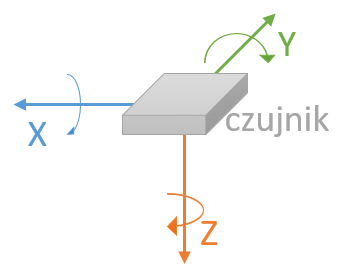
\includegraphics[width=0.5\textwidth]{images/IMUAxes.png}
		\caption{Układ współrzędnych dla czujników inercyjnych i~magnetycznych.}
		\label{fig:literature:imu:coordination}
	\end{figure}
\end{savenotes}

W swojej pracy Alexiev i Nikolova \cite{Alexiev2013} wyróżniają 4 klasy czujników inercyjnych ze względu na stopień zaszumienia ich pomiarów: nawigacyjne (oryg. \emph{navigation}), taktyczne  (oryg. \emph{tactical}), przemysłowe  (oryg. \emph{industrial}) oraz samochodowe  (oryg. \emph{automotive}). Poziom zaszumienia pomiarów czujników inercyjnych ma znaczący wpływ na to czy możliwe jest wystarczająco precyzyjne określenie położenia modułu inercyjnego w~przestrzeni wyznaczając metodami zliczeniowymi jego chwilowe przemieszczenie jedynie na podstawie pomiarów z jego czujników. Spowodowane jest to szybkim kumulowaniem się błędów, a co za tym idzie znacznym spadkiem dokładności w czasie. Tabla \ref{tab:acc:positionVsError} pokazuje przykład zaczerpnięty z \cite{Alexiev2013} jak szum pomiarów akcelerometru wpływa na dokładność oszacowania przemieszczenia się czujnika.

\begin{table}[]
	\centering
	\caption{Błąd estymacji położenia w zależności od błędu pomiarów akcelerometru\cite{Alexiev2013}.}
	\label{tab:acc:positionVsError}
	\begin{tabular}{|l|l|l|l|l|l|}
		\hline
		\rowcolor[HTML]{EFEFEF} 
		\cellcolor[HTML]{EFEFEF}                                 & \cellcolor[HTML]{EFEFEF}                                         & \multicolumn{4}{l|}{\cellcolor[HTML]{EFEFEF}Błąd szacowania położenia {[}m{]}} \\ \cline{3-6} 
		\rowcolor[HTML]{EFEFEF} 
		\multirow{-2}{*}{\cellcolor[HTML]{EFEFEF}Klasa czujnika} & \multirow{-2}{*}{\cellcolor[HTML]{EFEFEF}Błąd pomiarów {[}mg{]}} & 1 s     & 10 s  & 60 s & 1 hr    \\ \hline
		Nawigacyjne                                              & 0.025                                                               & 0.00013 & 0.012 & 0.44 & 1600    \\ \hline
		Taktyczne                                                & 0.3                                                                 & 0.0015  & 0.15  & 5.3  & 19000   \\ \hline
		Przemysłowe                                             & 3                                                                   & 0.015   & 1.5   & 53   & 190000  \\ \hline
		Samochodowe                                              & 125                                                                 & 0.62    & 60    & 2200 & 7900000 \\ \hline
	\end{tabular}
\end{table}

Jak widać z danych umieszczonych w tabeli \label{tab:acc:positionVsError}, uzyskanie dużej dokładności szacowania położenia stawów szkeletu ludzkiego za pomocą metod zliczeniowych wykorzystując pomiary czujników inercyjnych, jest zadaniem trudnym, a w długim czasie śledzenia może okazać się wręcz niemożliwe. Fakt ten ma więc wpływ na sposób budowania systemów śledzenia ruchu opartych na urządzeniach inercyjnych. W~przypadku śledzenia ruchu człowieka wymagane jest uzupełnienie pomiarów poprzez zdefiniowanie hierarchicznego modelu szkieletu ludzkiego, zawierającego informację o~długościach poszczególnych kości. Umożliwia to oszacowanie położenia poszczególnych stawów na podstawie orientacji czujników umieszczonych na poszczególnych częściach ciała. W~związku z~tym, duży wpływ na dokładność śledzenia ruchu w~systemach wykorzystujących czujniki inercyjne i~magnetyczne ma dokładność pomiaru długości poszczególnych kości.

Przykładem komercyjnej implementacji takiego systemu może być rozwiązanie zaproponowane przez firmę Xsens, które z~powodzeniem wykorzystywane jest zarówno do śledzenia ruchu na potrzeby animacji \footfullcite{footnote:XsensEnt}, jak i~do analizy ruchu u sportowców {\footfullcite{footnote:XsensSport1},\footfullcite{footnote:XsensSport2}}, czy w~procesie rehabilitacji motorycznej \footfullcite{footnote:XsensRehab}. Jednak na przykładzie zastosowań sportowych \footfullcite{footnote:XsensSport1, footnote:XsensSport2} należy zauważyć, że układy IMU i~MARG nie są wystarczające do zlokalizowania śledzonej postaci na scenie, a~jedynie do odtworzenia jej pozy. Aby śledzić aktualną lokalizację postaci wykorzystywany jest dodatkowy system umożliwiający określenie położenie postaci w~przestrzeni. W~zależności od tego na jak rozległej przestrzeni odbywa się ruch, może być to system GPS lub systemy oparte o~technologię LPM (\emph{ang. local position measurement}). GPS przeznaczony jest do lokalizowania obiektów, wyposażonych w odpowiedni odbiornik, na bardzo dużej otwartej przestrzeni (śledzony obiekt nie może być wewnątrz budynku), przy dokładności określenia położenia rzędu kilku metrów\footnote{Według danych zamieszczonych na \url{http://www.gps.gov/} dokładność systemu GPS może wynieść ok. $5m$ dla odbiorników wykorzystywanych na przykład w tlefonach komórkowych. Według wersji systemu, którego  odbiorniki wykorzystują komunikację na dwóch częstotliwościach równocześnie, uzyskiwana dokładność położenia jest rzędu kilku milimetrów}. Technologia LPM pozwalają na użycie ich zarówno wewnątrz budynków, jak i~na zewnątrz, wymagają jednak dodatkowych urządzeń obserwujących określony obszar, na którym odbywa się ruch. Jako przykład realizacji systemu LPM może posłużyć system firmy Inmotio\footfullcite{footnote:inmotio} wykorzysujący technologię radiową RFID (identyfikacja radiowa, \emph{ang. Radio-frequency identification}), która pozwala określić położenie śledzonej postaci na podstawie triangulacji pomiaru mocy sygnału pomiędzy stacjami bazowymi a~odbiornikiem. Przykładowa konfiguracja takiego systemu widoczna jest na rysunku \ref{fig:literature:footnote:inmotio:setup}). Szczegółowy opis działania systemu Xsens można znaleźć w~pracy Roetenberg i in. \cite{Roetenberg2009}.
					
\begin{savenotes}
	\begin{figure}[!htb]
		\centering	
		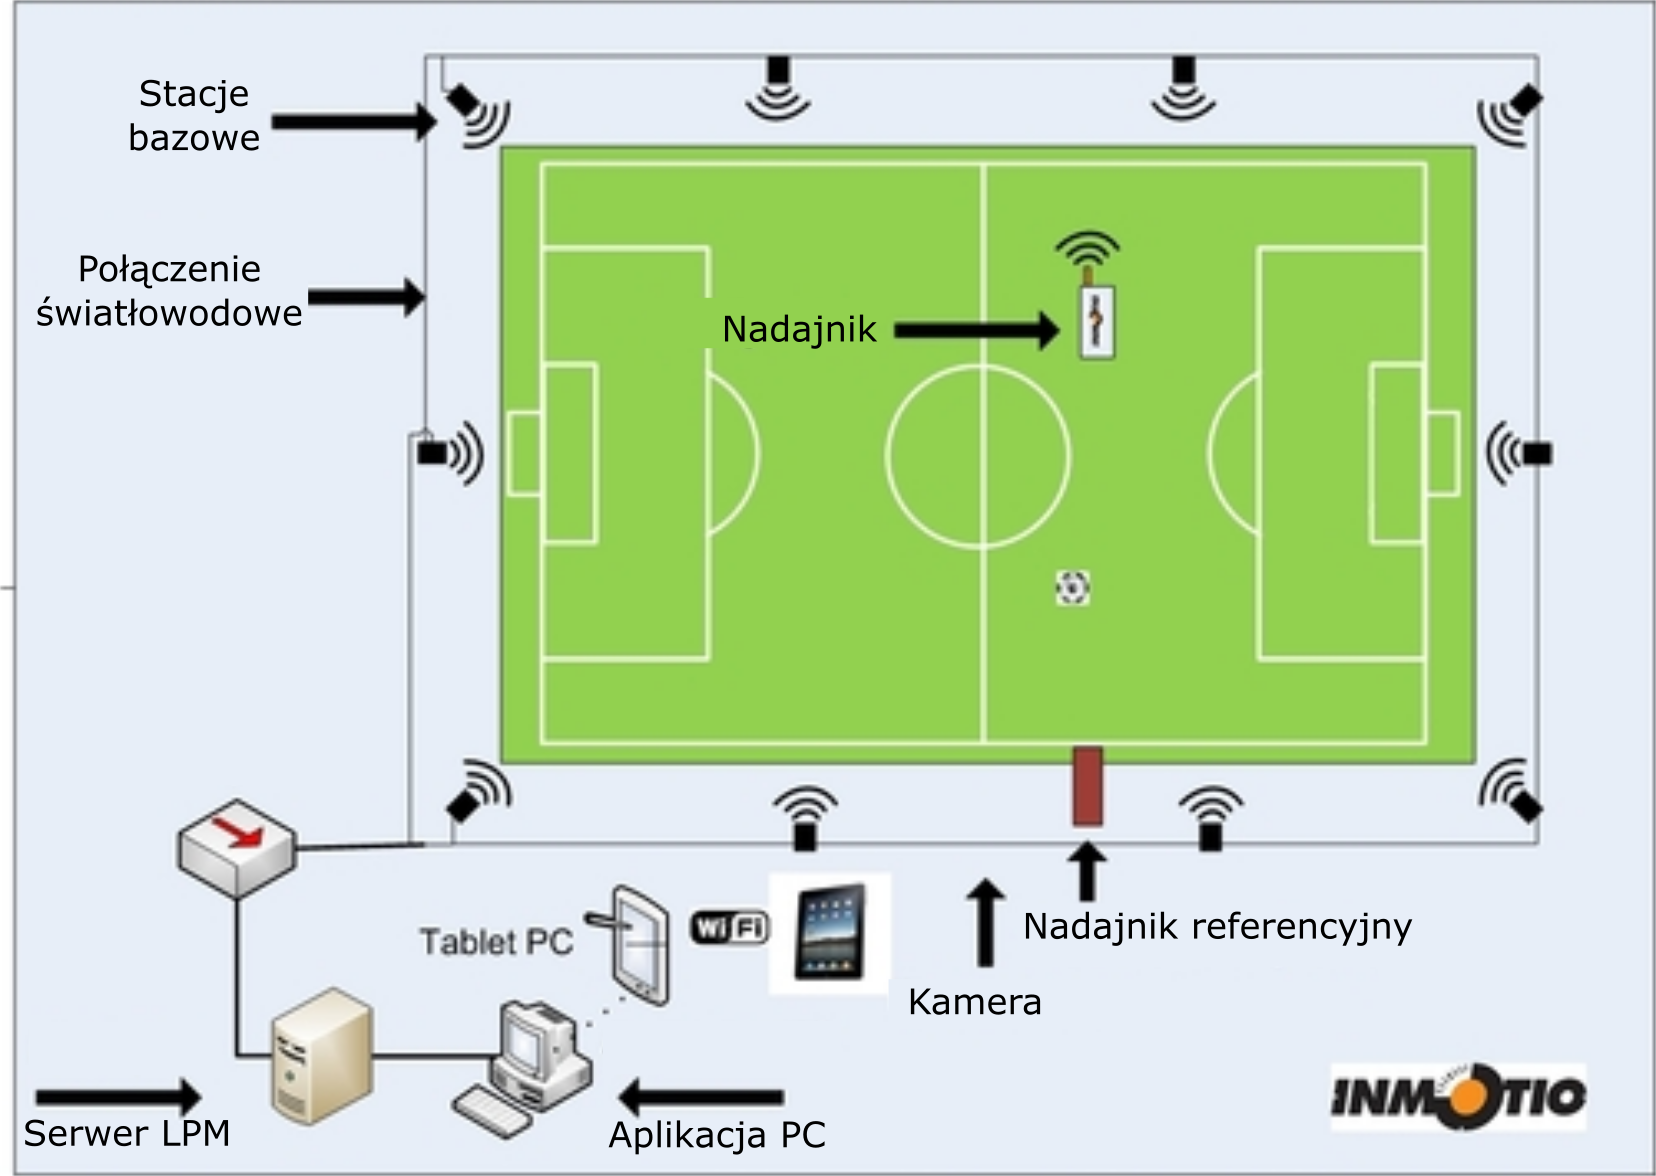
\includegraphics[width=0.75\textwidth]{images/lpm.png}
		\caption[Przykładowa konfiguracja systemu LPM firmy Inmotio]{Przykładowa konfiguracja systemu LPM firmy Inmotio\footfullcite{footnote:inmotio}}	
		\label{fig:literature:footnote:inmotio:setup}	
	\end{figure}
\end{savenotes}

Zmniejszenie zaszumienia pomiarów czujników inercyjych w celu poprawy dokładności szacowania pozycji stawów w inercyjnych i magnetycznych systemach śledzenia ruchu jest często spotykanym zagadnieniem w literturze naukowej. Oprócz wspomnianych już Alexieva i Nikolovej \cite{Alexiev2013}, którzy zaproponowali statystyczną metodę detekcji kiedy występuje prawdziwy ruch chujnika. Dzięki temu możliwe jest ograniczenie wpływu pomiarów złożonych jedynie z szumu, a to z kolei pozwala na spowolnienie spadku dokładności szacowania pozycji w czasie. Innym przykładem może być metoda przedstawiona przez Zhou i~Hu \cite{Zhou2005,Zhou2006}. Zaproponowali oni, na podstawie badań opartych o śledzenia ruchu stawów ręki, wykorzystanie algorytmu symulowanego wyżarzania w~celu zmniejszenia błędów pomiarowych czujników oraz zastosowali rozszerzony filtr Kalmana do połączenia sygnałów z~sensorów. Zaproponowaną przez siebie metodę, Zhou i~Hu przetestowali wykorzystując komercyjny, inercyjny system śledzenia ruchu firmy Xsens, natomiast dane referencyjne uzyskali za pomocą wizyjnego systemu śledzenia ruchu firmy Vicon. Zaproponowana przez nich metoda pozwoliła na poprawienie dokładności śledzenia ruchu stawów ręki o~$26\%$ z~około $2.3 cm$ do $1.7 cm$.
							
W przypadku systemów śledzenia ruchu człowieka opartych o~IMU i~MARG wpływ na dokładność wyznaczenia położenia poszczególnych stawów ma umiejscowienie czujników na ciele. Badania na ten temat prowadzili m.in. Vanegas i~Stirling \cite{Vanegas2015}. Badania te wykazały, że optymalnym miejscem umieszczenia tego typu sensorów są okolice środka masy danej części ciała lub obiektu. W~przypadku umieszczenia czujników na ciele człowieka pomocne okazują się być wyniki badań prowadzonych w~połowie lat 90-tych przez Paolo de Leva z~Uniwersytetu stanu Indiana. De Leva w~swojej pracy, dotyczącej badań nad środkami mas poszczególnych części ciała\cite{DeLeva1996}, rozwinął wcześniejsze badania Zatsiorskiego i~Seluyanova \cite{549} i~wyznaczył położenie poszczególnych środków mas kości. Rysunek \ref{fig:centerOfMass} przedstawia diagram rozmieszczenia środków mas dla każdej z~części ciała według badań de Leva.
							
\begin{savenotes}
	\begin{figure}[!htb]
		\centering	
		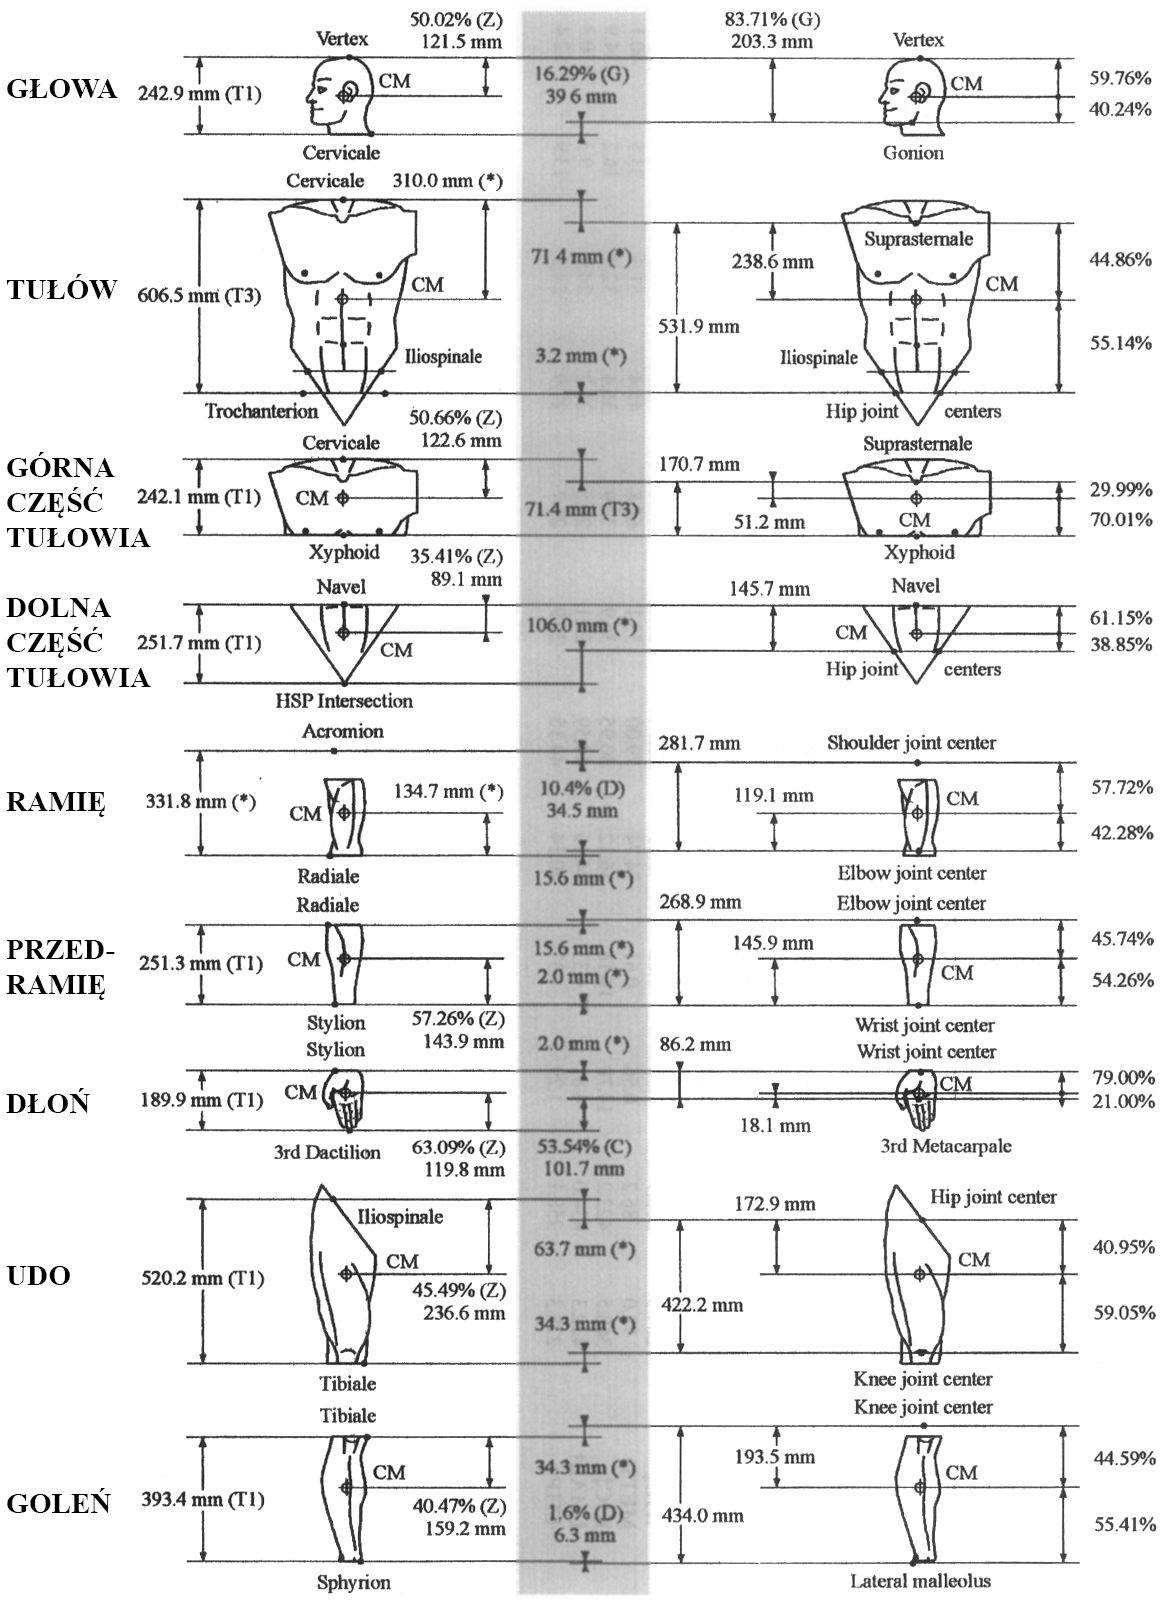
\includegraphics[width=0.95\textwidth]{images/centerOfMass.png}
		\caption[Rozmieszczenie środków mas poszczególnych części ciała człowieka według propozycji de Leva]{Rozmieszczenie środków mas poszczególnych części ciała człowieka według propozycji de Leva\cite{DeLeva1996}}	
		\label{fig:centerOfMass}	
	\end{figure}
\end{savenotes}
									
\subsubsection*{Systemy elektromagnetyczne (radiowe)}
Elektromagnetyczne systemy śledzenia ruchu opierają się o~pomiar strumienia elektromagentycznego wytworzonego między nadajnikiem umieszczonym na ciele postaci, której ruch jest śledzony, a~odbiornikami, które otaczają obszar, na którym odbywa się śledzenie ruchu. Zarówno nadajnik jak i~odbiorniki zbudowane są z~kilku prostopadłych cewek, co pozwala na śledzenie ruchu w~6 stopniach swobody (położenie oraz obroty). Dokładne położenie nadajnika w~przestrzeni wyznaczone jest za pomocą triangulacji uzyskiwanych pomiarów. Elektromagnetyczne systemy śledzenia ruchu są podatne na zakłócenia wynikające z~obecności elementów metalowych lub magnetycznych w~pobliżu obszaru, na którym odbywa się śledzenie. W~szczególności źródłem  takiego zakłócenia mogą być stalowe elementy konstrukcyjne budynku gdzie znajduje się system śledzenia (np. pręty zbrojeniowe w~stropie czy ścianach). Przykładem systemu śledzenia ruchu opartego o~tę technologię mogą być produkty firmy Polhemus na przykład system Patriot\footfullcite{footnote:Polhemus}
									
\subsubsection*{Systemy akustyczne}
Akustyczne systemy śledzenia opierają się na pomiarze czasu przemieszczania się fali dźwiękowej między nadajnikami umieszczonymi na ciele osoby, której ruch był śledzony, a~odbiornikami umieszczonymi wokół obszaru, na którym ruch się odbywał. Systemy te również określają położenie nadajników na podstawie triangulacji. Niestety, są one podatne na wiele czynników naturalnych, które mogą wpływać na dokładność uzyskanych wyników. Do takich czynników należą między innymi temperatura powietrza, wilgotność, czy ciśnienie atmosferyczne. Wymienione czynniki zewnętrzne powodują zmianę szybkości przemieszczania się fali dźwiękowej i w konsekwencji, zaburzenia rozchodzenia się dźwięku. Akustyczne systemy śledzenia ruchu zazwyczaj wykorzystują ultradźwięki, więc są niesłyszalne dla człowieka. Jednym z producentów systemów śledzenia opartych o ultradźwięki jest firma Nexonar\footfullcite{footnote:Nexonar}, której produkty zostały wykorzystane między innymi w~systemie wspomagającym naukę gry w golfa: Science and Motion\footnote{Science and Motion: \url{http://www.scienceandmotion.com/}}.
									
\subsubsection*{Systemy mechaniczne}
Mechaniczne systemy śledzenia ruchu różnią się znacznie od poprzednio opisanych systemów choćby ze względu na ich ingerencję w~swobodę ruchu jaki może wykonać śledzona osoba. Podstawowym urządzeniem wykorzystywnym w~mechanicznych systemach śledzenia ruchu, jest strój nazywany egzoszkieletem, zbudowany z~szeregu czujników mechanicznych i~elektromechanicznych, np. potencjometrów, których zadaniem jest odzwierciedlenie pozy jaką przyjmuje śledzona osoba. Przykładem egzoszkieletu może być układ mechaniczny będący elementem systemu śledzenia ruchu Gypsy \footfullcite{footnote:gypsy}. Egzoszkielet został~zaprezentowany na rysunku \ref{fig:literature:footnote:gypsy:full}.
									
\begin{savenotes}
	\begin{figure}[!htb]
		\centering	
		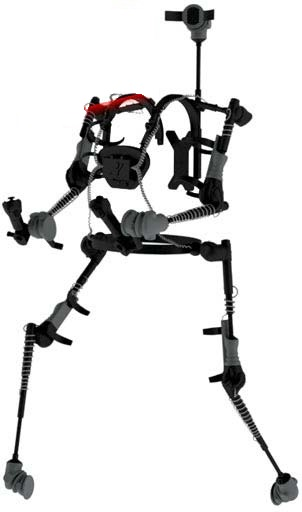
\includegraphics[height=6cm]{images/gypsy7_full.jpg}
		\caption{Egzoszkielet dla systemu MoCap Gypsy}	
		\label{fig:literature:footnote:gypsy:full}
	\end{figure}
\end{savenotes}
											
Niewątpliwą zaletą mechanicznych systemów śledzenia ruchu jest to, że głównym urządzeniem z~jakiego się składa taki system to wspomniany egzoszkielet. Nie jest on podatny na zakłócenia swojego działania przez elementy znajdujące się w~otoczeniu, czy przysłanianie się części ciała w~trakcie ruchu. Mechaniczne systemy śledzenia ruchu zazwyczaj są w~stanie pracować w~czasie rzeczywistym. Niestety, wadą jest, wspomniane już wcześniej, ograniczenie swobody wykonywanego ruchu, co powoduje, że nie każdy rodzaj ruchu (np. dynamiczne ćwiczenia gimnastyczne) może być śledzony za pomocą układów mechanicznych .
											
\section{Komputerowy model postaci ludzkiej} \label{chap:bodyRep}
Systemy śledzenia ruchu kończyn człowieka opierają się często na komputerowym modelu postaci, który opisuje właściwości kinematyczne modelu szkieletu oraz, jeśli to możliwe, również kształt ciała śledzonej postaci. Reprezentacja geometryczna opisująca zewnętrzny wygląd postaci jest zmapowana na jego układ szkieletowy, dzięki czemu zmiany szkieletu mogą być automatycznie przekładane na zewnętrzną pozę postaci, natomiast na podstawie kształtu i~ustawienia ciała człowieka można wnioskować jaka jest konfiguracja szkieletu. 
Nie istnieje jeden standardowy model postaci, gdyż w~zależności od zastosowań przyjmowane sa różne uproszczenia. O ile szkielet kostny dorosłego człowieka składa się z~206 kości \cite{Lasinski1990}, o~tyle w~modelach komputerowych, na potrzeby rejestracji ruchu, stosuje się ich zazwyczaj kilkadziesiąt. Przykładowo, model szkieletowy zastosowany w~kontrolerze Kinect składa się z~20 stawów i~19 kości\footfullcite{footnote:msdn:kinectSkeleton}, zaś model szkieletowy systemu Optitrack zbudowany jest również z~20 stawów, ale połączonych ze sobą za pomocą 25 kości\footfullcite{footnote:optitrackSkeleton} (zwiększona liczba kości w~obrębie klatki piersiowej oraz stóp). Zatem przyjęcie właściwego modelu reprezentacji postaci wpływa na swobodę ruchów (liczba stopni swobody) modelowanego układu kostnego, co z kolei przekłada się na skuteczność i~dokładność śledzenia kończyn człowieka.
											
\subsection{Model kinematyczny szkieletu postaci}
Model kinematyczny szkieletu postaci opisany jest za pomocą struktury przedstawiającej relacje między poszczególnymi stawami połączonymi ze sobą segmentami reprezentującymi kości. Każdy ze stawów opisany jest przez tzw. stopnie swobody definiujące w~jaki sposób segmenty (kości) połączone danym stawem mogą się wzajemnie poruszać. Teoretycznie maksymalna liczba stopni swobody danego stawu może wynosić 6, co oznacza, że staw może przesunąć się wzdłuż każdej z~3 osi $X, Y$ i~$Z$ układu współrzędnych oraz obracać się wokół każdej z~nich, jednak w~praktyce zakres ruchomości stawów człowieka jest ograniczony i~osobniczo różny. W~związku z~tym pozycja każdego ze stawów jest determinowana stopniem swobody jego rodzica. Zatem wiedząc, że staw łokciowy ma jeden stopień swobody, ruch kości przedramienia jest ograniczony tylko do jednej płaszczyzny, a~względna możliwa pozycja stawu nadgarstkowego znajduje się na łuku o~promieniu równym długości kości przedramienia.

Model kinematyczny jest zazwyczaj definiowany jako hierarchiczny układ stawów co oznacza, że wielkości opisujące dany staw są wielkościami względnymi w~odniesieniu do stawu bezpośrednio go poprzedzającego (nadrzędnego) w~hierarchii. Aby wyznaczyć wartości absolutne danego stawu, niezbędne jest przyrostowe złożenie informacji ze wszystkich stawów w~łańcuchu kinematycznym, począwszy od stawu głównego (korzenia). Korzeniem nazywamy jeden wyszczególniony staw modelu hierarchicznego, do którego doczepione są łańcuchy kinematyczne wszystkich pozostałych stawów. Korzeń może, ale nie musi mieć swojego odpowiednika w~stawach szkieletu ludzkiego. Jako przykład można przytoczyć propozycję uproszczonego modelu szkieletowego człowieka wraz z~przedstawieniem hierarchii poszczególnych segmentów oraz ich stopni swobody zaproponowaną przez Kwolek i in.\cite{Kwolek2014} i~przedstawioną na rys. \ref{fig:literature:skeletonModelHierarchy}. W~modelu kinematycznym, w~którym określona jest hierarchia jego stawów, układ współrzędnych, w~którym opisane są obroty i~położenie danego stawu, ma swój początek w~stawie poprzedzającym go (staw rodzica). Sprawia to, że wartości przypisane do poszczególnych stawów są wielkościami względnymi.
											
\begin{savenotes}
	\begin{figure}[!htb]
		\centering
		\begin{minipage}{.18\textwidth}
			\centering
			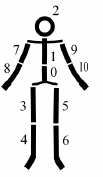
\includegraphics{images/hierarchical-structure.png}       
		\end{minipage}%
		\hfill
		\begin{minipage}{0.75\textwidth}
			\centering
			\scalebox{0.73}{
				\tiny
\begin{tikzpicture}[
	level 1/.style={sibling distance=5.3cm},
level 2/.style={sibling distance=2.3cm}, 
	every node/.style = {shape=rectangle, rounded corners,
    draw, align=center}]]
  \node {0. Miednica\\(\emph{ang. Pelvis})\\6 DOF}   
    child { node {3. Lewe udo\\(\emph{ang. Upper Right Leg})\\2 DOF}
    	child { node {4. Lewy piszczel\\(\emph{ang. Right Lower Leg})\\1 DOF}}
    }
    child { node {1. Kręgosłup\\(\emph{ang. Spine})\\3 DOF}    	
    	child {node{7. Prawe ramię\\(\emph{ang. Upper Right Arm})\\3 DOF}
    		child {node{8. Prawe przedramię\\(\emph{ang. Right Forearm})\\1 DOF}}
    	}
    	child {node{2. Głowa\\(\emph{ang. Head})\\3 DOF}}
	child {node{9. Lewe ramię\\(\emph{ang. Upper Left Arm})\\3 DOF}
		child {node{10. Lewe przedramię\\(\emph{ang. Left Forearm})\\1 DOF}}
	}	     
    }
    child { node {5. Prawe udo\\(\emph{ang. Upper Left Leg})\\2 DOF}
    	child { node {6. Prawy piszczel\\(\emph{ang. Left Lower Leg})\\1 DOF}}
    };
\end{tikzpicture}
			}
		\end{minipage}
		\caption[Uproszczony hierarchiczny model szkieletowy człowieka wraz z~diagramem przedstawiającym hierarchię poszczególnych elementów]{Uproszczony hierarchiczny model szkieletowy człowieka (lewo) wraz z~diagramem przedstawiającym hierarchię poszczególnych elementów(prawo) \cite{Kwolek2014}}
		\label{fig:literature:skeletonModelHierarchy}
	\end{figure}
\end{savenotes}
													
Oprócz stopni swobody pojedynczego stawu, definiuje się również stopień swobody całego modelu kinematycznego. Taka wielkość rozumiana jest jako suma stopni swobody wszystkich jego elementów. W~przypadku pełnego opisu modelu postaci możemy mieć zatem do czynienia z~modelem kinematycznym, który posiada zdefiniowanych ponad 50 stopni swobody \cite{Agarwal2006}. Nie zawsze jednak potrzebne są modele zawierające pełen opis stopni swobody. Okazuje się, że do śledzenia większości ruchów człowieka wystarczający jest model uproszczony definiujący około 30 stopni swobody \cite{Sigal2006,Kwolek2011}.
													
O ile model kinematyczny szkieletu jest w~stanie jednoznacznie opisać pozę, w~jakiej znajduje się śledzona postać w~danej chwili czasu o~tyle może okazać się to niewystarczające w~przypadku śledzenia ruchu w~środowiskach wirtualnych, w~których istotna jest interakcja postaci z~otoczeniem. W~takim przypadku niezbędne staje się określenie dodatkowo modelu kształu ciała śledzonej postaci.
															
\subsection{Model reprezentacji postaci}
Modele kształtu ciała, podobnie jak modele kinematyczne, możemy określać w~przestrzeni dwu-- lub trójwymiarowej. Zwykle wystarczające jest przybliżone odwzorowanie kształtu poszczególnych części ciała za pomocą figur geometrycznych (modele 2D) lub brył (modele 3D). Pozwala to zwizualizować budowę ciała postaci, której ruch jest śledzony, bez zbytniego obciążania procesora komputera, na którym odbywa się przetwarzanie danych pozyskanych z~systemu śledzenia. Dokładne odwzorowanie budowy ciała postaci jest możliwe dzięki wykorzystaniu popularnych przestrzennych reprezentacji geometrycznych (np.: siatka trójkątna 3D), jednak ich wykorzystanie może wpłynąć negatywnie na wydajność systemu. 
Niezależnie jakie reprezentacje geometryczne wykorzystujemy, istotne jest takie przedstawienie kształtu ciała, aby odpowiednio zwizualizować przynajmniej śledzone ruchy. Przykładowo, jeśli wykorzystujemy trójwymiarowy uproszczony model zbudowany z~kul i~cylindrów trudne będzię zwizualizowanie niektórych obrotów ciała, przykładowo rotacji dłoni i~nadgarstka jak na rys. \ref{fig:literature:wristRotation}.
															
\begin{savenotes}
	\begin{figure}[!htb]
		\centering	
		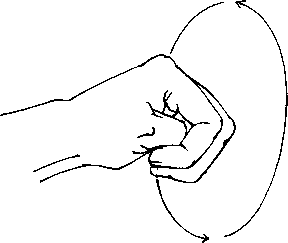
\includegraphics[height=6cm]{images/Wrist_joint_rotation.png}
		\caption{Rotacja wewnętrzna (pronacja) i~zewnętrzna (supinacja) dłoni\footfullcite{footnote:wristRotation}}	
		\label{fig:literature:wristRotation}
	\end{figure}
\end{savenotes}
															
W praktyce to w~jaki sposób aktor będzie reprezentowany w~systemie komputerowym ściśle powiązane jest z~przeznaczeniem danego systemu. Inna reprezentacja będzie konieczna dla śledzenia i~rozpoznawania pozy w~jakiej znajduje się aktor, a~inaczej jeśli śledzimy jego położenie w~przestrzeni. I~tak możemy wyróżnić następujące sposoby reprezentowania postaci:
																
\begin{itemize}
	\item \textbf{punkt} -- postać reprezentowana jest przez pojedynczy punkt (zazwyczaj środek ciężkości) \cite{Veenman2001} lub kilka punktów określających punkty charakterystyczne na ciele \cite{Serby2004}. Reprezentacja taka jest zazwyczaj użyteczna jeśli śledzony obiekt zajmuje niewielki fragment obszaru, na którym odbywa się śledzenie;
	\item \textbf{figury i~bryły geometryczne} -- śledzona postać może być reprezentowana przez pojedynczą figurę/bryłę \cite{Comaniciu2003} lub kilka brył odpowiadających za każdą cześć ciała. W~tej reprezentacji wykorzystuje się proste figury/bryły, które mogą jednoznacznie zobrazować śledzone ciało. Do takich możemy zaliczyć między innymi: prostokąty, elipsy, cylindry, prostopadłościany;
	\item \textbf{sylwetka} -- w~przypadku tej reprezentacji możliwe są dwa warianty realizacji: jako kontur pusty lub jako kontur z~wypełnieniem. Dodatkowo, sam obrys może być pełny, czyli zrealizowany jako figura zamknięta zaznaczona linią ciągłą, lub przedstawiony jedynie jako zbiór punktów kluczowych na obrysie sylwetki. Taka reprezentacja została zaproponowana między innymi w~\cite{Yilmaz2004}, do śledzenia interakcji człowieka z~obiektami o~nieregularnych kształtach;
	\item \textbf{szkielet} -- model szkieletowy jest niejako graficzną reprezentacją modelu kinematycznego. Jest to hierarchiczna struktura zbudowana z~prostych figur/brył geometrycznych i~swoim kształtem oddaje pozycję w~jakiej znajduje się śledzona postać. Szkielet taki powinien być w~stanie w~pełni zawrzeć się w~obrysie postaci \cite{Ali2001}. Chociaż zwyczajowo punkty, z~których zbudowany jest model szkieletowy nazywa się stawami (\emph{ang. joints}), nie muszą one odpowiadać stawom w~szkielecie biologicznym. Na przykład, często występujący w~modelu szkieletowym staw reprezentujący kość miedniczą lub głowę, w rzeczywistości nie istnieje;
\end{itemize}
															
W niniejszej pracy wykorzystywana jest trójwymiarowa reprezentacja szkieletowa modelu 3D śledzonej postaci złożona z~20 stawów i~19 segmentów kości. Model ten przedstawiony jest na rysunku \ref{fig:characteristics:kinect:skeleton}. W~zależności od wykorzystywanego systemu śledzenia ruchu inna jest metoda wyznaczania położenia i~obrotów poszczególnych stawów. W~dalszej części zamieszczony został opis metod związanych z~technikami śledzenia wykorzystywanymi w~niniejszej pracy. To jest: optyczny system śledzenia ruchu z~markerami pasywnymi, inercyjny system śledzenia ruchu oraz optyczny system śledzenia ruchu bez markerów.

\begin{savenotes}
	\begin{figure}[!htb]	
			\centering
			\scalebox{0.73}{													
		\begin{tikzpicture}
	\node (leyend) at (7, 0){
		\begin{tabular}{l@{: }l}
			10 & Środek bioder   \\
			11 & Kręgosłup      \\
			12 & Środek barków  \\
			13 & Głowa           \\
																																																																																																																				 	
			20 & Lewe biodro      \\
			21 & Lewe kolano      \\
			22 & Lewa kostka      \\
			23 & Lewa stopa       \\
																																																																																																																				 	
			30 & Prawe biodro     \\
			31 & Prawe kolano     \\
			32 & Prawa kostka     \\
			33 & Prawa stopa      \\
																																																																																																																				 	
			40 & Lewy bark        \\
			41 & Lewy łokieć    \\
			42 & Lewy nadgarstek  \\
			43 & Lewa dłoń      \\
																																																																																																																				 	
			50 & Prawy bark       \\
			51 & Prawy łokieć   \\
			52 & Prawy nadgarstek \\
			53 & Prawa dłoń     
																																																																																																																				 	
		\end{tabular} };
																																																												
	\tikzset{
		joint/.style	= {draw, very thin, circle}
	}
																																																													
	\draw  
	node at (0,0) [joint, fill=gray!40](hipCenter){10}
																																																													
	node at (-1,-1) [joint, fill=green!40](hipLeft){20}
	node at (-1.5,-3.5) [joint, fill=green!40](kneeLeft){21}
	node at (-1.5,-6)[joint, fill=green!40](ankleLeft){22}
	node at (-2.5,-6.5)[joint, fill=green!40](footLeft){23}
																																																													
	node at (1,-1)[joint, fill=blue!40](hipRight){30}
	node at (1.5,-3.5)[joint, fill=blue!40](kneeRight){31}
	node at (1.5,-6)[joint, fill=blue!40](ankleRight){32}
	node at (2.5,-6.5)[joint, fill=blue!40](footRight){33}
																																																													
	node at (0,1) [joint, fill=gray!40](spine){11}
																																																													
	node at (0,4) [joint, fill=gray!40](shoulderCenter){12}
																																																													
	node at (-1,3.5) [joint, fill=red!40](shoulderLeft){40}
	node at (-1.7,1.5) [joint, fill=red!40](elbowLeft){41}
	node at (-1.9,-0.5) [joint, fill=red!40](wristLeft){42}
	node at (-2.4,-1.3)[joint, fill=red!40](handLeft){43}
																																																													
	node  at (1,3.5) [joint, fill=yellow!40](shoulderRight){50}
	node at (1.7,1.5) [joint, fill=yellow!40](elbowRight){51}
	node at (1.9,-0.5) [joint, fill=yellow!40](wristRight){52}
	node at (2.4,-1.3) [joint, fill=yellow!40](handRight){53}
																																																													
	node  at (0,5.5)[joint, fill=gray!40](head){13};
																																																													
	\draw
	(head) -- (shoulderCenter)
																																																													
	(shoulderCenter) -- (shoulderLeft) -- (elbowLeft) -- (wristLeft) -- (handLeft)        
	(shoulderCenter) -- (shoulderRight) -- (elbowRight) -- (wristRight) -- (handRight)  
	(shoulderCenter) -- (spine)
																																																													
	(spine) -- (hipCenter)
																																																													
	(hipCenter) -- (hipLeft) -- (kneeLeft) -- (ankleLeft) -- (footLeft)        
	(hipCenter) -- (hipRight) -- (kneeRight) -- (ankleRight) -- (footRight);
\end{tikzpicture}
			}
		\caption{Model szkieletowy człowieka wykorzystywany w~kontrolerze Microsoft Kinect}
		\label{fig:characteristics:kinect:skeleton}
	\end{figure}
\end{savenotes}		
													
\subsection{Wyznaczanie położenia stawów w~modelu szkieletowym}
Metody wyznaczania położenia oraz obrotu stawów w~modelu szkieletowym mogą się znacząco od siebie różnić w~zależności od zastosowanego systemu śledzenia ruchu. W~przypadku systemów wykorzystujących markery możemy przyjąć, że podstawową różnicą (pomijając wykorzystywanie różnych zjawiskach fizycznych, takich jak fala elektromagnetyczna, czy fala akustyczna) jest to, czy oszacowane położenie danego stawu jest wynikiem jego bezpośredniego śledzenia (bądź śledzenia markerów przymocowanych w~sąsiedztwie tego stawu), czy jest to efekt przekształceń geometrycznych wynikających ze śledzenia ruchu markerów umieszczonych blisko środków ciężkości kości, pomiędzy dwoma kolejnymi stawami. W~przypadku systemów śledzenia ruchu niewykorzystujących markerów, wyznaczenie położenia stawów odbywa się przy wykorzystaniu analizy i~rozpoznawania obrazów postaci, na podstawie których wnioskuje się położenie poszczególnych stawów.
																	
\subsubsection*{Wyznaczanie położenia stawów w~optycznych systemach śledzenia ruchu z~markerami}
Optyczne systemy śledzenia ruchu kończyn stosujące markery, są przykładem systemów, w~którym określenie położenia stawów odbywa się przez śledzenie ruchu markerów bezpośrednio przymocowanych do ciała śledzonej postaci. Aby możliwe było określenie położenia oraz obrotu danego stawu, każdy staw musi być oznaczony przez minimum 2 markery. Komercyjnie dostępne, optyczne systemy śledzenia ruchu stosujące markery posiadają zazwyczaj zdefiniowane schematy rozmieszczenia markerów na ciele człowieka, tak aby móc na ich podstawie automatycznie określić niezbędne paramtery dla każdego ze stawów. Rysunek \ref{fig:literature:vicon:markerPlacement} przedstawia przykładowy schemat rozmieszczenia markerów wykorzystany w~systemie śledzenia firmy Vicon. Szczegółowy opis akronimów wykorzystanych do oznaczenia markerów można znaleźć w~dokumentacji systemu Vicon \cite{ViconGaitPlacement}.
																	
\begin{savenotes}
	\begin{figure}[!htb]
		\centering	
		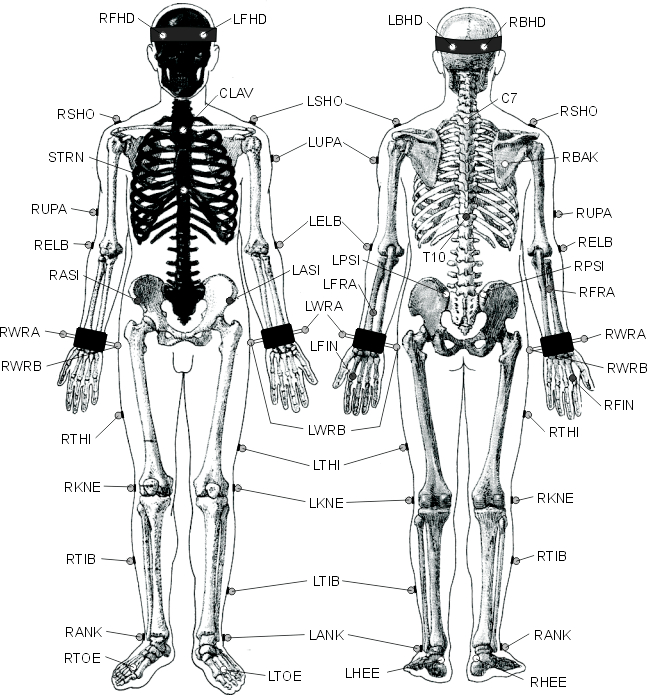
\includegraphics[width=0.75\textwidth]{images/markerPlacement.jpg}
		\caption[Rysunek przedstawiający schemat umieszczania markerów na ciele człowieka w~systemie śledzenia ruchu firmy Vicon]{Schemat umieszczania markerów na ciele człowieka w~systemie śledzenia ruchu firmy Vicon\cite{ViconGaitPlacement}}
		\label{fig:literature:vicon:markerPlacement}
	\end{figure}
\end{savenotes}
																			
Kolejnym krokiem po wyznaczeniu położenia poszczególnych markerów, na podstawie obrazów z~kamer, jest interpretacja tych danych w~taki sposób, aby uzyskać opis stanu stawów, które są reprezentowane graficznie przez pojedyncze punkty posiadajace informacje nie tylko o~swoim położeniu, ale także orientacji przestrzennej. Interpretacja ta odbywa się bądź to na podstawie obliczeń matematycznych, wynikających wprost z~położenia przestrzennego wyznaczonych punktów i~relacji między nimi, lub na podstawie przyjętego modelu biomechanicznego ciała ludzkiego. 

Przykładem sposobu wyznaczania położenia stawu na podstawie wzajemnej relacji pomiędzy stawami, może być proces wyznaczania położenia kości miedniczej (\emph{ang. pelvis}). Rysunek \ref{fig:literature:vicon:pelvisPlacement} pokazuje umiejscowienie markerów wykorzystywanych do wyznaczenia pozycji stawu reprezentującego kość miedniczą. Według dokumentacji \cite{ViconModelingInstruction} położenie kości miedniczej jest szacowane jako średnia arytmetyczna punktów RASI i~LASI (rys. \ref{fig:literature:vicon:pelvisPlacementA}). Jeśli jeden z~tych dwóch punktów jest niewidoczny, wówczas położenie stawu reprezentującego kość miedniczą jest wyznaczane jako wierzchołek trójkąta prostokątnego, którego przeciwprostokątną wyznaczają punkty SACR oraz jeden z~widocznych RASI lub LASI.
																	
\begin{savenotes}
	\begin{figure}[!htb]
		\centering
																																
		\begin{subfigure}[b]{0.45\textwidth}
			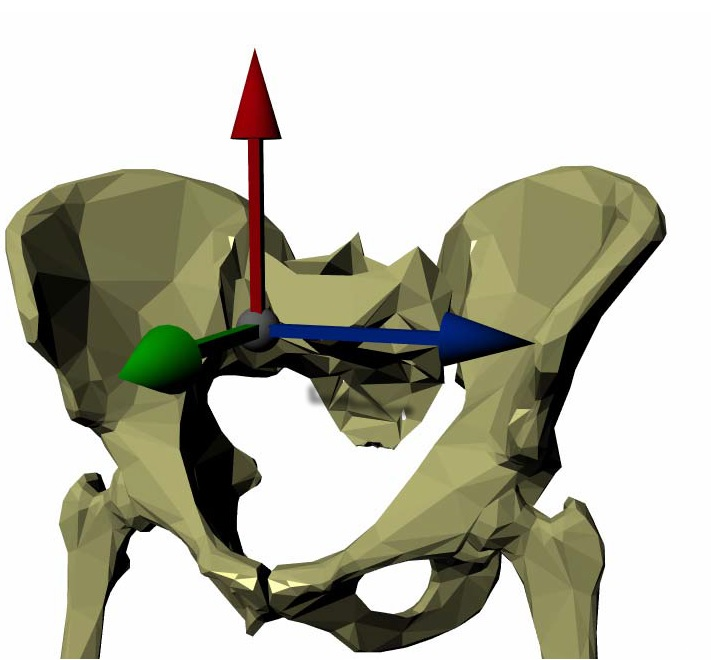
\includegraphics[width=\textwidth]{images/pelvisEstimationB.jpg}		
			\caption{Położenie wyznaczonego stawu kości miedniczej}
			\label{fig:literature:vicon:pelvisPlacementB}
		\end{subfigure}
		\hfill	
			\begin{subfigure}[b]{0.45\textwidth}
			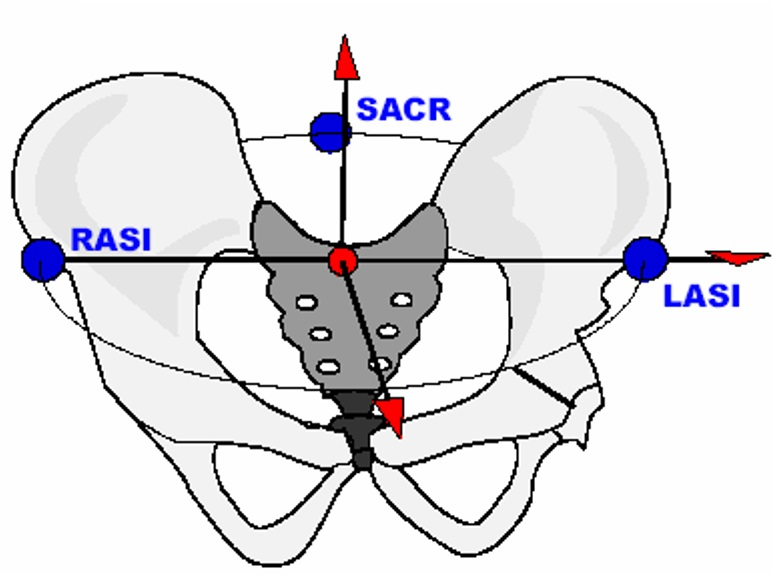
\includegraphics[width=\textwidth]{images/pelvisEstimationA.jpg}	
			\caption{Położenie markerów}
			\label{fig:literature:vicon:pelvisPlacementA}
		\end{subfigure}

		\caption[Wyznaczenie położenia kości miedniczej na potrzeby modelu szkieletowego na podstawie położenia markerów w~systemie Vicon]{Rysunek przedstawiający wyznaczenie położenia kości miedniczej (a) na potrzeby modelu szkieletowego na podstawie położenia markerów (b) w~systemie Vicon\cite{ViconModelingInstruction}}
		\label{fig:literature:vicon:pelvisPlacement}
	\end{figure}
\end{savenotes}
																			
Przykładem wyznaczania położenia stawu modelu szkieletowego na podstawie biomachanicznego modelu szkieletu ludzkiego, może być schemat wyznaczania położenia stawów biodrowych. Opierając się na pracy Davies i in. \cite{Davis1991} do wyznaczenia położenia stawów zostały wykorzystane informacje o~szerokości miednicy, długości kości udowej postaci, której ruch jest śledzony, oraz współczynników skalujących i~stałych zdefiniowanych we wspomnianej pracy. Równania \ref{eq:hipEquation:Xcoordinate}--\ref{eq:hipEquation:Zcoordinate} przedstawiają przykład wyznaczania współrzędnych położenia dla prawego biodra.
																					
\begin{subequations}
	\begin{align}
		X & = f_C * \cos(\gamma) * \sin(\upsilon) - (f_h + f_m) * \cos(\upsilon) \label{eq:hipEquation:Xcoordinate} \\
		Y & = -(f_C * \sin(\gamma) - f_a) \label{eq:hipEquation:Ycoordinate}                                        \\
		Z & = -f_C * \cos(\gamma)*\cos(\upsilon) - (f_h + f_m) * \sin(\upsilon) \label{eq:hipEquation:Zcoordinate}  
	\end{align}
	\label{eq:hipEquation:XYZcoordinates}
\end{subequations}
																					
Przyjmując, że $l_l$ i~$l_p$ to długości kości udowych obu nóg, współczynnik $f_C$ zdefiniowany jest empirycznie według wzoru \ref{eq:hipEquation:Ccoeficient}.
																					
\begin{equation}
	\centering
	f_C = \frac{l_l + l_p}{2} * 0.115 - 15.3
	\label{eq:hipEquation:Ccoeficient}
\end{equation}
																					
Współczynnik $f_h$ wyznaczany jest na podstawie wartości $l_l$ albo $l_p$ w~zależności czy wyznaczane jest położenie biodra dla lewej albo prawej strony. Współczynnik $f_h$ zdefiniowany został według wzoru \ref{eq:hipEquation:Hcoeficient}.
																					
\begin{equation}
	\centering
	f_h = 0.1288 * l_p - 48.56
	\label{eq:hipEquation:Hcoeficient}
\end{equation}
																					
Współczynnik $f_a$ wyznaczony jest jako połowa odległości pomiędzy stawem kości miedniczej a~położeniem markera LASI albo RASI, natomiast współczynnik $f_m$ określa średnicę markerów wykorzystywanych w~trakcie śledzenia. Kąty $\gamma$ oraz $\upsilon$ przyjmują stałe wartości odpowiednio $0.5\quad rad$ oraz $0.314\quad rad$. W~dokumentacji systemu śledzenia Vicon\cite{ViconModelingInstruction} można również znaleźć opisy procedur wyznaczania położenia dla pozostałych stawów.
																			
\subsubsection*{Wyznaczanie położenia stawów w~inercyjnych i~magnetycznych systemach śledzenia ruchu}
Inercyjne i~magnetyczne systemu śledzenia ruchu wymagają nieco innego podejścia do wyznaczania położenia poszczególnych stawów, ponieważ nie udostępniają one bezpośrednio informacji dotyczących ich położenia w~przestrzeni, a~jedynie orientację oraz wartości sił działających na poszczególne czujniki. Pozwala to określić przyspieszenie i~kierunek z~jakim porusza się czujnik (akcelerometr) oraz prędkość z~jaką się obraca (żyroskop). Dzięki wykorzystaniu pomiarów poszczególnych czujników inercyjnych, możliwe jest zastosowanie metod zliczeniowych do określenia przybliżonego położenia wynikającego z przemieszczenia się obiektu, do którego dany czujnik jest przymocowany \cite{HyeRiPark2009, Montorsi2013b}. Uzyskanie dokładnego położenia danego czujnika wymaga wykorzystania drogich komponentów, w~których zaszumienie danych pomiarowych jest stosunkowo niewielkie. W~przypadku powszechnie dostępnych czujników inercyjnych wykorzystywanych przykładowo w~telefonach, czy w~inercyjnych systemach śledzenia ruchu, takich jak XSense, czujniki inercyjne wykorzystywane są do określenia orientacji przestrzennej takiego czujnika, czy kształtu pozy jaką przyjęła w~danej chwili śledzona osoba. Konsekwencją takiego podejścia jest to, że korzeń modelu szkieletowego w~systemie śledzenia ruchu opartym o~czujniki inercyjne i~magnetyczne pozostaje zazwyczaj nieruchomy. 

Możliwe jest zdefiniowanie tylko fragmentu modelu szkieletowego, zawierającego przykładowo ramię i~przedramię prawej ręki, którego korzeniem będzie staw barkowy. Wówczas cały model zbudowany będzie z~3 stawów, jednego nieruchomego odpowiadającego stawowi barkowemu i~dwóm ruchomym: łokciowemu i~nadgarstkowemu.
																			
W inercyjnych i~magnetycznych systemach śledzenia ruchu markery wyposażone w~odpowiednie czujniki umieszczane są na powierzchni ciała osoby (wzdłuż kości), której ruch jest śledzony. Czujniki inercyjne działają najlepiej jeśli umieszczone są blisko środka masy poruszającego się obiektu. Wyznaczeniem środków mas kości człowieka zajmują się między innymi badacze z~zakresu biomechaniki, a~przykładem efektów tych prac może być diagram wyznaczający środki mas kości zaprezentowany w~pracy Paolo de Leva \cite{DeLeva1996} i przedstawiony na rysunku \ref{fig:centerOfMass}.
																					
\begin{savenotes}
	\begin{figure}[!htb]
		\centering	
		\includegraphics[width=0.75\textwidth]{images/imuArm.png}
		\caption[Przykładowy schemat umieszczenia markerów inercyjnych na potrzeby śledzenia ruchu ręki]{Przykładowy schemat umieszczenia markerów inercyjnych na potrzeby śledzenia ruchu ręki. Niebieskie prostokąty oznaczają schematyczne zamieszczenie czujników inercyjnych, zaś zielone kropki oznaczają symbolicznie pozycję stawów szkieletu ramienia. }
		\label{fig:literature:imuMarkerPlacementSample}
	\end{figure}
\end{savenotes}
																							
Rysunek \ref{fig:literature:imuMarkerPlacementSample} pokazuje przykładowy sposób umieszczenia markerów inercyjnego systemu śledzenia ruchu na powierzchni ręki, tak aby ich położenie możliwie pokrywało się ze środkiem mas poszczególnych segmentów kończyny. Moduły inercyjne, dostarczające informacje o~swojej orientacji w~przestrzeni, nie przekazują wprost informacji o~położeniu konkretnych stawów, a~jedynie określają jaki obrót, względem jakiegoś stanu początkowego, wykonała kończyna, do której te moduły zostały przymocowane. Posługując się przykładowym schematem z~rysunku \ref{fig:literature:imuMarkerPlacementSample}, przyjmijmy staw barkowy (punkt 3 z rys. \ref{fig:literature:imuMarkerPlacementSample}) jako korzeń. Chcąc określić położenie stawu łokciowego (punkt 4 z rys. \ref{fig:literature:imuMarkerPlacementSample}), niezbędna jest informacja o~orientacji przestrzennej modułu inercyjnego umieszczonego na ramieniu (prostokąt 1 z rys. \ref{fig:literature:imuMarkerPlacementSample}), oraz długość kości ramieniowej, która łączy stawy barkowy i~łokciowy. Mając te dwie informacje należy dokonać obrotu wektora o~długości takiej, jak długość kości ramieniowej, do orientacji, w~jakiej znajduje się rozważany moduł (prostokąt 1 z rys. \ref{fig:literature:imuMarkerPlacementSample}). Wówczas punkt początkowy hierarchicznego modelu szkieletowego ręki reprezentuje staw barkowy i~znajduje się w~umownym punkcie $(0 , 0 , 0)$, natomiast punkt końcowy reprezentuje staw łokciowy, a~jego współrzędne $(X , Y , Z)$ odpowiadają położeniu tego stawu w~przestrzeni. Wyznaczenie położenia stawu nadgarstkowego (punkt 5 z rys. \ref{fig:literature:imuMarkerPlacementSample}) odbywa się analogicznie, przy czym punktem nadrzędnym jest położenie stawu łokciowego (punkt 4 z rys. \ref{fig:literature:imuMarkerPlacementSample}), a,~modułem którego orientacja jest brana pod uwagę, jest sensor umieszczony na przedramieniu (prostokąt 2 z rys. \ref{fig:literature:imuMarkerPlacementSample}). W~przypadku systemów śledzenia ruchu wykorzystujących moduły inercyjne istotne jest zachowanie hierarchii stawów wykorzystywanego modelu szkieletowego i~wykonywanie obliczeń zgodnie z~tą hierarchią.
																							
\subsubsection*{Wyznaczanie położenia stawów modelu szkieletowego w~optycznym, bezmarkerowym systemie śledzenia ruchu}\label{chap:humanModel:kinect}
Optyczne, bezmarkerowe systemy śledzenia ruchu, w głównej mierze, opierają się na analizie i rozpoznawaniu rejestrowanego obrazu w celu wyodrębnienia elementów, których ruch będzie śledzony. Elementy takie można wówczas interpretować jako wirtualne znaczniki, bo w istocie system śledzenia jedynie na ich podstawie odtwarza model szkieletu postaci. Na przykładzie kotrolera Microsoft Kinect można przedstawić jeden z~możliwych sposobów wyznaczania modelu postaci przez oprogramowanie wykorzystywane w~systemie śledzenia ruchu nie bazującym na markerach, lecz stosującym algorytmy rozpoznawania obrazów. Algorytm zastosowany w~kontrolerze Kinect jest w~stanie rozpoznać tylko szkielet postaci ludzkiej, a~w~zależności od trybu pracy szkielet ten przedstawia całą sylwetkę albo jedynie jej górną część, na którą składają się głowa, ręce oraz barki. Należy zwrócić uwagę, że model szkieletowy przedstawiający pełną sylwetkę, jest jedynie modelem uproszczonym zawierającym 20 stawów (rys. \ref{fig:characteristics:kinect:skeleton}).
																							
Kontroler Kinect wykorzystuje mechanizm uczenia maszynowego, dzięki któremu możliwe jest rozpoznawanie poszczególnych części ciała śledzonej postaci na podstawie obrazu mapy głębi. Zastosowana w~kontrolerze metoda uczenia maszynowego opiera się na algorytmie losowych lasów decyzyjnych\cite{Criminisi2011}, który podlegał wcześniejszemu procesowi uczenia. W~celu nauczenia algorytmów decyzyjnych, zastosowanych w~kontrolerze Kinect, przygotowano bazę ponad miliona wzorców różnych póz, w~jakich może się znajdować śledzona postać wraz z~oznaczonymi częściami ciała. Zestaw zdjęć zastosowany do uczenia algorytmu składał się z~blisko stu tysięcy zdjęć póz rzeczywistych postaci, uzupełnionych pomiarami z~systemu śledzenia ruchu o~wysokiej dokładności oraz z~kilkuset tysięcy wzorcowych zdjęć cyfrowych postaci wygenerowanych (wyrenderowanych) komputerowo\cite{MacCormick2011}. Odpowiednio wytrenowany algorytm zyskał gotowość do rozpoznawania i~klasyfikowania elementów przedstawionego obrazu jako części ciała człowieka. Wykorzystując między innymi wzajemne położenie elementów (pojedyncze punkty lub grupy punktów -- obszary) występujących na mapie głębi, algorytm szacuje, które z~nich należą do tej samej części ciała. Efektem działania algorytmu losowych lasów decyzyjnych jest tzw. mapa części ciała (ang. \emph{body parts map}), której przykład przedstawiony jest jako drugi krok na schemacie widocznym na rysunku \ref{fig:literature:kinect:classificationSteps}.
																							
\begin{savenotes}
	\begin{figure}[!htb]
		\centering	
		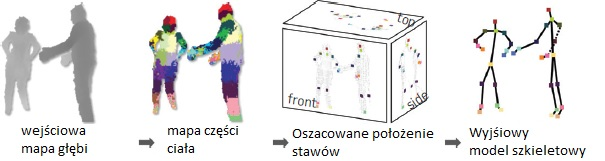
\includegraphics[width=0.75\textwidth]{images/KinectRecognitionSteps.jpg}
		\caption{Schemat przedstawiający kolejne kroki wyznaczania modelu szkieletowego na podstawie mapy głębi.}
		\label{fig:literature:kinect:classificationSteps}
	\end{figure}
\end{savenotes}
																									
Mapa części ciała stanowi podstawę dla kolejnego kroku wyznaczania modelu szkieletowego, jakim jest oszacowanie położenia stawów w~przestrzeni trójwymiarowej. Segmenty, z~których składa się mapa części ciała, przetworzone są algorytmem \emph{mean shift} \cite{Comaniciu2003}, co w~efekcie daje oszacowanie położenia poszczególnych stawów. Połączenie ich zgodnie ze zdefiniowaną hierarchią wyznacza model szkieletowy śledzonej postaci. Warto zaznaczyć, że większość tych operacji zaimplementowana została jako oprogramowanie wbudowane procesora firmy Prime Sense. Hipotetycznie, w~celu wykorzystania Kinecta do podobnego rozpoznawania innych obiektów, czy zwierząt, należałoby zaimplementować przedstawiony powyżej proces, opierając się na specjalnie przygotowanych do tego danych.

Warto zwrócić uwagę, że proces wyznaczania mapy głębi i~reprezentacji szkieletowej śledzonego użytkownika opiera się na danych pozyskanych tylko z~jednego układu, jaki stanowią kamera i~projektor światła podczerwonego (IR - \emph{ang. infra red}). Kamera RGB nie jest w~ogóle do tego zadania wykorzystywana, co z~kolei skutkuje tym, że urządzenie jest w~stanie działać w~zaciemnionych pomieszczeniach.
																									
Kinect wykorzystuje reprezentację ciała użytkownika w~postaci szkieletowej. Składa się ona z~20 jednopunktowych węzłów, które w~dużej mierze pokrywają się ze stawami ludzkiego szkieletu (rys. \ref{fig:characteristics:kinect:skeleton}). Każdy z~węzłów posiada swoje współrzędne w~przestrzeni trójwymiarowej związanej z~kontrolerem, wyrażone w~metrach, gdzie punktem (0,0,0) jest projektor podczerwieni w~kontrolerze Kinect. Rysunek \ref{fig:characteristics:kinect:space} przedstawia układ współrzędnych wykorzystywany w~Kinekcie do określenie położenia stawów. 
																									
\begin{savenotes}
	\begin{figure}
		\centering
		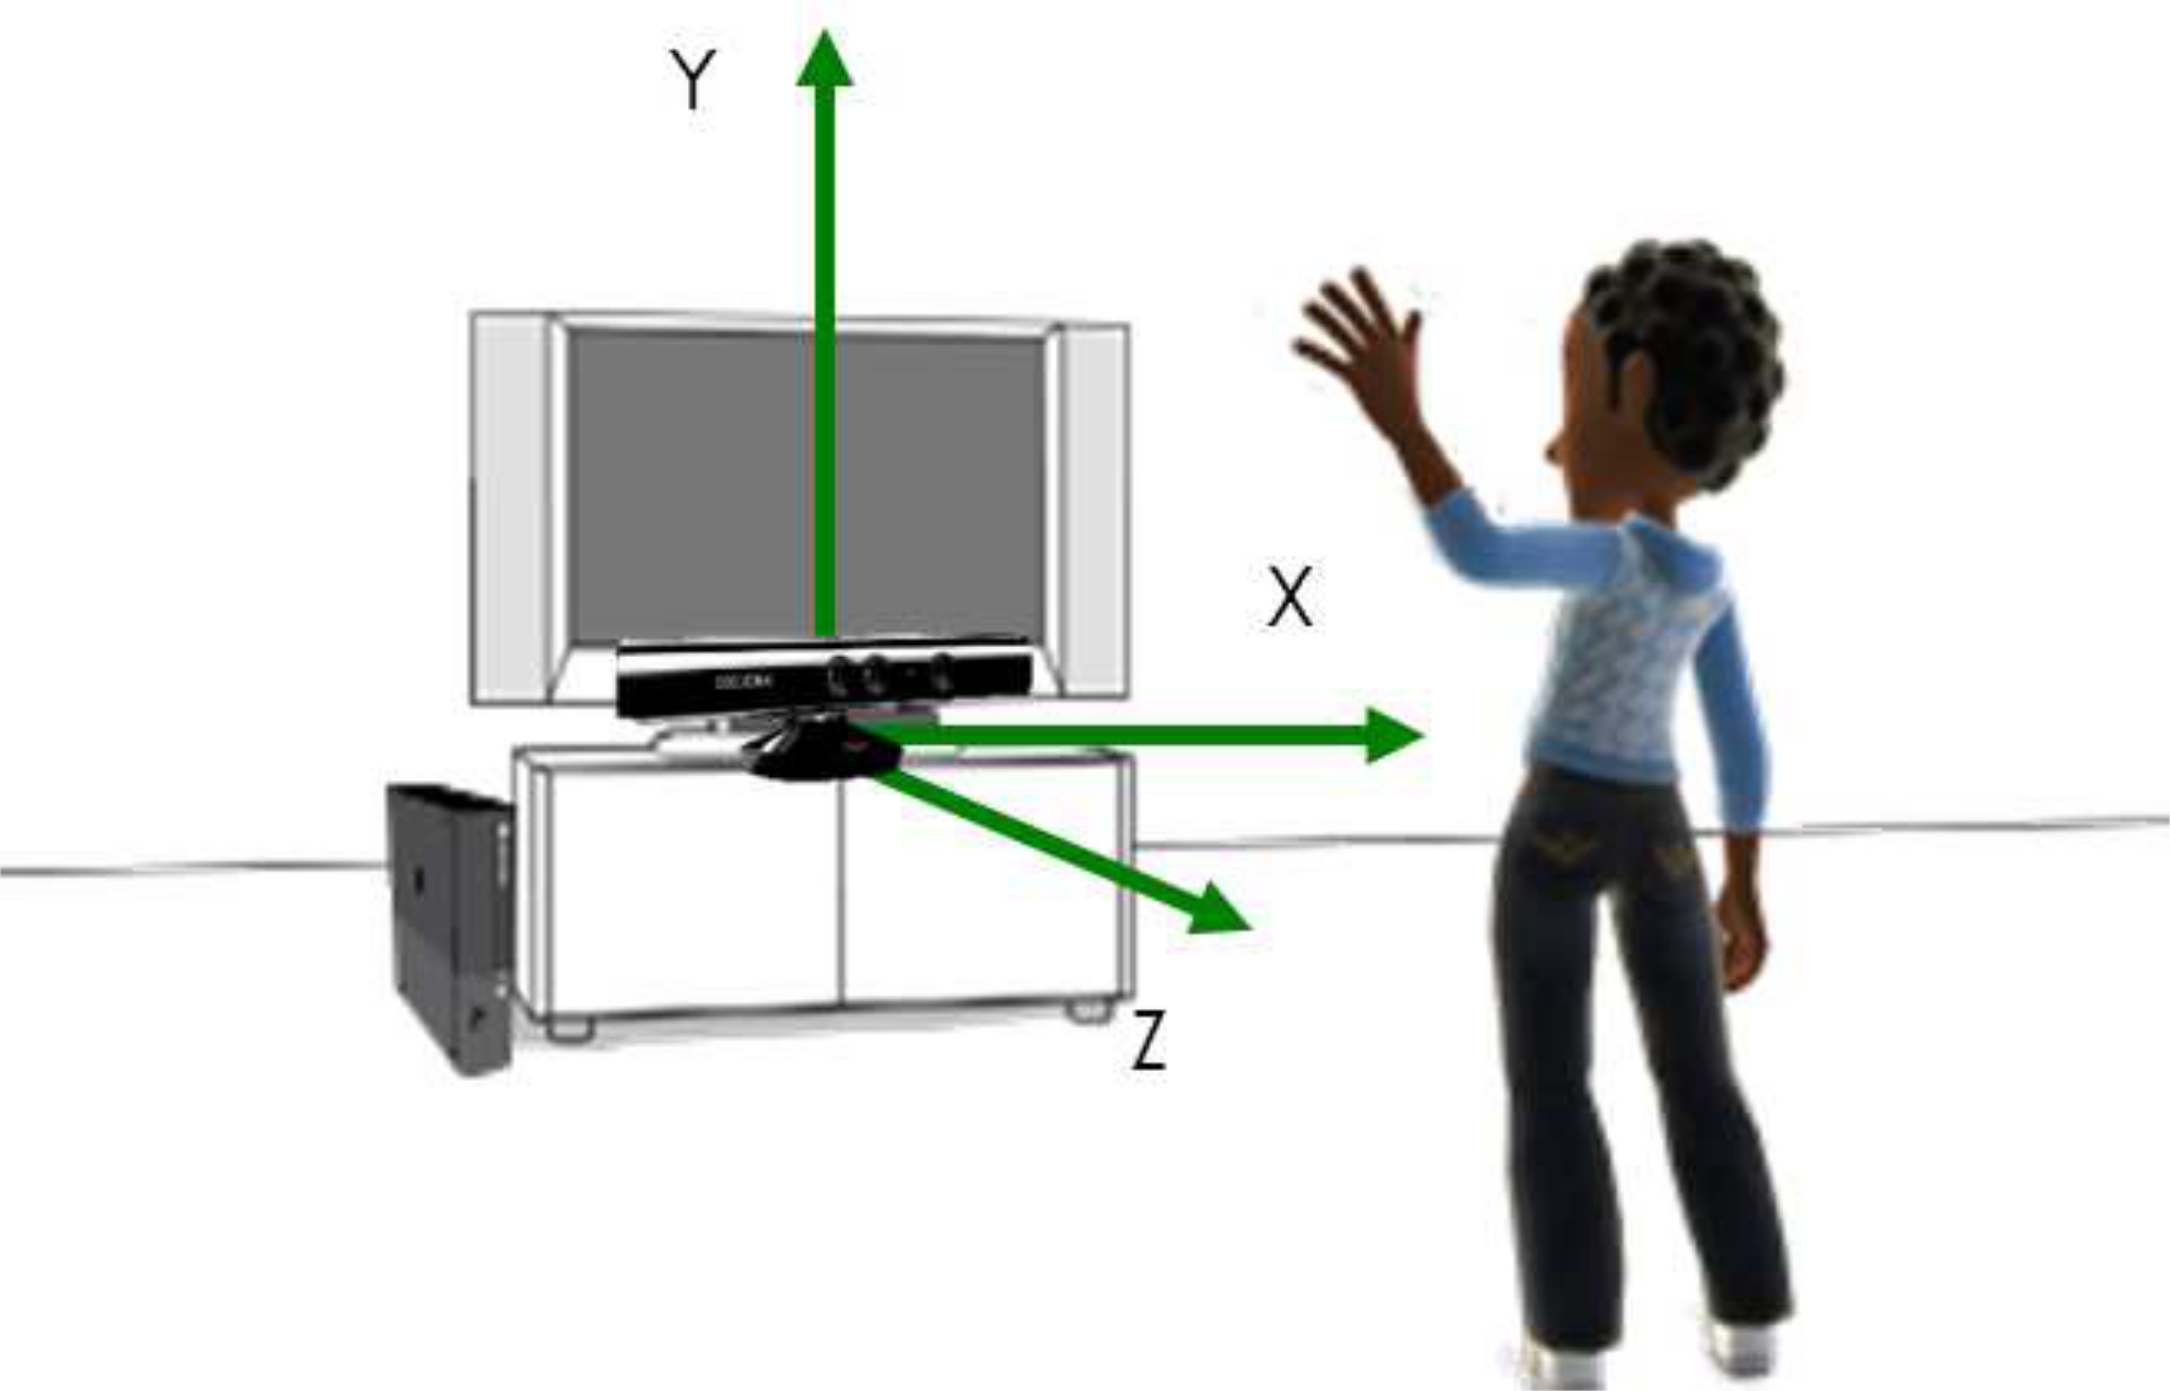
\includegraphics[width=0.6\textwidth]{images/skeletonSpace.png}
		\caption[Układ współrzędnych wykorzystywany w~kontrolerze Microsoft Kinect]{Układ współrzędnych wykorzystywany w~kontrolerze Microsoft Kinect \footfullcite{footnote:msdn:kinectCoordSpace2016}}
		\label{fig:characteristics:kinect:space}
	\end{figure}
\end{savenotes}
																											
																									
\subsection{Reprezentacja rotacji obiektu w~przestrzeni}\label{chap:orientstionRep}
Istnieje wiele metod reprezentowania orientacji obiektu w przestrzeni, i~każda z~tych metod wyróżnia się charakterystycznymi dla siebie cechami, które mogą wpływać na łatwość obliczeń kosztem czytelności zapisu bądź na optymalizację użycia pamięci przy~ich implementacji komputerowej. Do najpopularniejszych można zaliczyć następujące metody:
																										
\begin{itemize}
	\item Kąty Eulera,
	\item Macierze rotacji,
	\item Pary Osie-Kąt (\emph{ang. Axis--Angle}),
	\item Kwaterniony.
\end{itemize} 
																											
\subsubsection*{Kąty Eulera} \label{sec:orientstionRep:euler}
Reprezentacja orientacji obiektu za pomocą kątów Eulera jest najbardziej intuicyjną z~powszechnie używanych reprezentacji, ponieważ przedstawia ona 3 wartości kątów, o~jakie nastąpił obrót względem odpowiednich osi układów współrzędnych. Należy jednak pamiętać, że konwencje nazewnicze odnoszące się do poszczegónych kątów i osi różnią się w zależności od dziedziny w jakiej okreslana jest orientacja na przykład inych oznaczeń używa się w awiacji a innych w przypadku określenia obrotów kończyn w systemach śledzenia. Jest to związane z~układem odniesienia, jaki został przyjęty do określania obrotów. Możemy wyróżnić relatywny układ odniesienia, w~którym obrót mierzony jest względem arbitralnie wybranego układu (\emph{ang. body--fixed coordinate system}, rys.\ref{fig:appx:rot:eulerRel}), lub układ absolutny -- względem kierunków ziemi (\emph{ang. world coordinate system}, rys.\ref{fig:appx:rot:eulerAbs}). Tabela \ref{tab:appx:rot:eulerNames} zawiera powszechnie przyjęte konwencje oznaczania obrotów.
																													
\begin{savenotes}
	\begin{figure}[!htb]
		\captionsetup{singlelinecheck=off}
		\centering
		\begin{subfigure}[b]{0.63\textwidth}
			\centering
			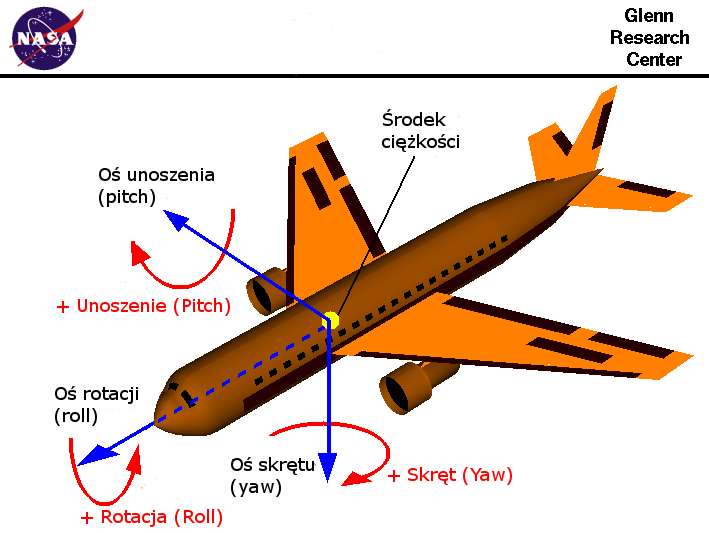
\includegraphics[width=\textwidth]{images/nasaAircraft.png}	
			\caption[Kąty Eulera w relatywnym układzie współrzędnych]{Relatywny \footfullcite{footnote:nasa2016}}
			\label{fig:appx:rot:eulerRel}
		\end{subfigure}
						\hfill																																						
		\begin{subfigure}[b]{0.35\textwidth}
			\centering
			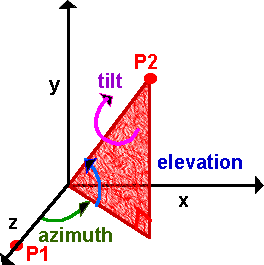
\includegraphics[width=\textwidth]{images/eulerAbsolute.png}		
			\caption[Kąty Eulera w absolutnym układzie współrzędnych]{Absolutny \footfullcite{footnote:Baker2015}}
			\label{fig:appx:rot:eulerAbs}
		\end{subfigure}
																																											
		\caption{Kąty Eulera względem przyjętego układu współrzędnych: relatywnego (a) oraz absolutnego (b)}
		\label{fig:appx:rot:euler}
	\end{figure}
\end{savenotes}
																											
																											
\begin{table}[!htb]
	\centering
	\caption{Konwencje nazewnicze kątów Eulera}
	\label{tab:appx:rot:eulerNames} 
	\begin{tabular}{|c|c|c|c|c|}
		\hline
		Oś & Układ Relatywny & Układ Absolutny & Symbol   & Prędkość kątowa \\
		\hline
		X   & \emph{bank}      & \emph{tilt}      & $\psi$   & \emph{roll}         \\
		Y   & \emph{heading}   & \emph{azimuth}   & $\theta$ & \emph{yaw}          \\ 
		Z   & \emph{attitude}  & \emph{elevation} & $\phi$   & \emph{pitch}        \\
		\hline
	\end{tabular} 
\end{table}
																													
Chcąc prawidłowo interpretować podane wartości trzeba pamiętać, że określają one zawsze obroty względem określonych osi w~ściśle określonej kolejności. Spośród 27\foottnote{osie w~sekwencji mogą się powtarzać więc na podstawie wzoru wariacji z powtórzeniami otrzymujemy $3^3 = 27$} możliwych kombinacji określających kolejność wykonywania rotacji wokół osi, jedynie 12 może być wykorzystane do zdefiniowania obrotów w~przestrzeni 3D \cite{Diebel2006}. Ograniczenie ilości możliwych do wykorzystania sekwencji obrotów, wynika z założenia, że dwa następujące po sobie obroty nie mogą być wykonane wokół tej samej osi. Dokładne opisy sekwencji wykonywanych obrotów można znaleźć w~pracach poświęconych zagadnieniu rotacji obiektów \cite{Pio1966, Diebel2006}. Innym utrudnieniem, które trzeba brać pod uwagę w~przypadku stosowania kątów Eulera wyrażonych w relatywnym układzie współrzędnych, jest występowanie niejednoznaczności przy obrotach w~orientacji pionowej ($ \phi=\pm90\degree $). W~takim wypadku wykonanie dowolnej innej rotacji powoduje niejednoznaczność względem której osi odbył się ruch. Sytuacja, o~której jest mowa nosi angielską nazwę \emph{gimbal lock}. W~przypadku implementacji komputerowej, taki przypadek wymaga szczególnej obsługi w~celu uniknięcia błędów zarówno interpretacyjnych jak i~matematycznych.
																													
\subsubsection*{Macierze orientacji}
Reprezentacja orientacji w~postaci kątów Eulera jest intuicyjna z~punktu widzenia interpretacji przez człowieka, ale utrudnia ona obliczanie obrotów na bieżąco. W~takim przypadku należy ją skonwertować do innej postaci -- dobrze sprawdzają się tu macierze obrotów względem każdej z~osi, opisane wzorami \ref{eq:appx:rot:rMatrix:rx}, \ref{eq:appx:rot:rMatrix:ry} oraz \ref{eq:appx:rot:rMatrix:rz}.
																													
\begin{subequations}
	\begin{align}
		\mathbf{R_x(\alpha)} & = 
		\begin{bmatrix}
		1            & 0            & 0            \\
		0            & cos(\alpha)  & sin(\alpha)  \\
		0            & -sin(\alpha) & cos(\alpha)  
		\end{bmatrix} 
		\label{eq:appx:rot:rMatrix:rx} \\				
		\mathbf{R_y(\alpha)} & = 
		\begin{bmatrix}
		cos(\alpha)  & 0            & -sin(\alpha) \\
		0            & 1            & 0            \\
		sin(\alpha)  & 0            & cos(\alpha)  
		\end{bmatrix} 
		\label{eq:appx:rot:rMatrix:ry} \\				
		\mathbf{R_z(\alpha)} & = 
		\begin{bmatrix}
		cos(\alpha)  & sin(\alpha)  & 0            \\
		-sin(\alpha) & cos(\alpha)  & 0            \\
		0            & 0            & 1            
		\end{bmatrix} 
		\label{eq:appx:rot:rMatrix:rz}
	\end{align}
\end{subequations}
																													
Rotacja o~dowolne kąty względem każdej z~osi rozumiana jest jako iloczyn powyższych macierzy. Końcowa postać macierzy obrotu będąca wynikiem takiego iloczynu wyrażona jest wzorem \ref{eq:appx:rot:rMatrix:all}.
																													
\begin{equation}
	\footnotesize
	\begin{split}
		&\mathbf{R(\phi,\theta,\psi)} = \mathbf{R_z(\psi)}\mathbf{R_y(\theta)}\mathbf{R_x(\phi)} =\\
		&=	\begin{bmatrix}
		cos(\theta)cos(\psi)   & cos(\phi)sin(\psi) + cos(\phi)sin(\theta)cos(\psi) & sin(\phi)sin(\psi) - cos(\phi)sin(\theta)cos(\psi) \\
		-cos(\theta)sin(\psi)  & cos(\phi)cos(\psi) - sin(\phi)sin(\theta)sin(\psi) & sin(\phi)cos(\psi) + cos(\phi)sin(\theta)sin(\psi) \\
		sin(\theta)            & 			-sin(\phi)cos(\theta) 		            & cos(\phi)cos(\theta)            
		\end{bmatrix} 
		\label{eq:appx:rot:rMatrix:all}
	\end{split}
\end{equation}
																														
\subsubsection*{Pary Osie-Kąt (\emph{ang. Axis--Angle})}
Reprezentacja orientacji w~postaci pary Osie-Kąt odpowiada za określenie kierunku (osie) oraz wielkości obrotu (kąt). Zapisuje się ją jak we wzorze \ref{eq:appx:rot:angleAxis:form}
																												
\begin{equation}
	\alpha\mathbf{e} = (\alpha, \begin{bmatrix}e_1 & e_2 & e_3\end{bmatrix})
	\label{eq:appx:rot:angleAxis:form}
\end{equation}
																													
przy założeniu, że wektor $\mathbf{e}$ jest wektorem o~długości 1. 
Forma ta jest zbliżona do reprezentacji kwaternionowej, jednak nie można używać jej w~obliczeniach z~podobną łatwością.  
																													
\subsubsection*{Kwaterniony}
Ostatnią z~prezentowanych reprezentacji orientacji obiektu są kwaterniony. Są to liczby z~ciała liczb zespolonych, składające się z~części rzeczywistej oraz części urojonej. Część urojona reprezentowana jest przez 3 liczby określające wektor obrotu, zaś część rzeczywista składa się z jednej liczby określającej kąt obrotu wokół danego wektora obrotu. Jej zaletą jest łatwość i~zwięzłość zapisu operacji obrotu obiektu oraz składania sekwencji obrotów. Obarczone jest to jednak utrudnioną interpretacją tego zapisu przez człowieka. Aby na podstawie kwaternionu określić pod jakim kątem w~stosunku do poszczególnych osi układu znajduje się obiekt, należy dokonać szeregu operacji arytmetycznych. Ogólna postać kwaternionu wyrażona jest jak we wzorze \ref{eq:appx:rot:quat}:
																													
\begin{equation}
	\label{eq:appx:rot:quat}
	\mathbf{q} =
	\begin{bmatrix}
		q_0 \\
		q_1 \\
		q_2 \\
		q_3 
	\end{bmatrix} 
	= 	
	\begin{bmatrix}
		q_w \\
		q_x \\
		q_y \\
		q_z 
	\end{bmatrix} 
	= 
	\begin{bmatrix}
		cos(\frac{\alpha}{2})    \\
		e_1sin(\frac{\alpha}{2}) \\
		e_2sin(\frac{\alpha}{2}) \\
		e_3sin(\frac{\alpha}{2}) 
	\end{bmatrix}
\end{equation}
gdzie $q_{0-1}, q_{w-z}, e_{1-3} \in \mathbb{R}, \alpha \in [-\pi \pi], \sqrt{e_1^2 + e_2^2 + e_3^2} = 1$
																													
Wartości kąta $\alpha$ oraz $e_{1-3}$ są tożsame z~reprezentacją w~postaci Osie-Kąt.
																													
Wzór \ref{eq:appx:rot:quat} nie wyczerpuje wszystkich reprezentacji kwaternionów jakie występują w~literaturze. Widać na nim jednak, że określenie o~ile stopni obrócono obiekt jest przynajmniej trudne. Wybierając notację dla zapisu kwaternionów należy szczególnie zadbać o~określenie, która z~wartości w~wektorze odpowiada za część rzeczywistą, a~które za część urojoną. W~niniejszej pracy część rzeczywista reprezentowana jest przez element wektora oznaczony indeksem $0$ lub $w$. Wzór \ref{eq:appx:rot:quat} pokazuje też związek pomiędzy kwaternionem a~reprezentacją w~postaci pary Osie-Kąt.
																													
Aby skutecznie dokonywać obliczeń za pomocą kwaternionów muszą być one znormalizowane, czyli spełniać zależność $\|\mathbf{q}\| = 1$.
																													
Opis operacji matematycznych oraz geometrycznych jakie wykonywane mogą być na kwaternionach można znaleźć w~szeregu publikacji (np. \cite{Dantam2014}) na ten temat, a~także w~podręcznikach akademickich dotyczących matematyki.
																													
\subsubsection*{Konwersje}
Dla każdej z~powyższych reprezentacji orientacji istnieje możliwość dokonania konwersji na dowolną inną. Taka operacja może być przydatna jeśli chcemy przykładowo prezentować aktualną orientację obiektu użytkownikowi, a~postać, która jest używana przy obliczeniach nie jest intuicyjnie interpretowalna przez człowieka. Z~uwagi na to, że w~niniejszej pracy do wyrażenia orientacji i~obrotów wykorzystane były dwie formy reprezentacji: kąty Eulera oraz kwaterniony, konwersja pomiędzy tymi dwoma reprezentacjami została przedstawiona poniżej.
																													
\subsubsection*{Kąty Eulera $\rightarrow$ Kwaternion}
Przyjmując, że kąty Eulera wyrażone są przez sekwencję obrotów $Z-Y-X$ (\emph{ang. Tait–Bryan angles}), konwersja z~reprezentacji za pomocą kątów Eulera do reprezentacji za pomocą kwaternionów wyrażona jest wzorem \ref{eq:appx:rot:eulerToQuat}
																													
\begin{equation}
	\label{eq:appx:rot:eulerToQuat}
	\begin{bmatrix}
		q_w \\
		q_x \\
		q_y \\
		q_z 
	\end{bmatrix} 
	= 
	\begin{bmatrix}
		\cos{\frac{\psi}{2}}\cos{\frac{\theta}{2}}\cos{\frac{\phi}{2}}+\sin{\frac{\psi}{2}}\sin{\frac{\theta}{2}}\sin{\frac{\phi}{2}} \\
		\cos{\frac{\psi}{2}}\cos{\frac{\theta}{2}}\sin{\frac{\phi}{2}}-\sin{\frac{\psi}{2}}\sin{\frac{\theta}{2}}\cos{\frac{\phi}{2}} \\
		\cos{\frac{\psi}{2}}\sin{\frac{\theta}{2}}\cos{\frac{\phi}{2}}+\sin{\frac{\psi}{2}}\cos{\frac{\theta}{2}}\sin{\frac{\phi}{2}} \\
		\sin{\frac{\psi}{2}}\cos{\frac{\theta}{2}}\cos{\frac{\phi}{2}}-\cos{\frac{\psi}{2}}\sin{\frac{\theta}{2}}\sin{\frac{\phi}{2}} 
	\end{bmatrix}
\end{equation}
																													
\subsubsection*{Kwaternion $\rightarrow$ Kąty Eulera}
Przy analogicznych założeniach co do sekwencji kątów Eulera, konwersja z~postaci kwaternionowej wyrażona jest wzorem \ref{eq:appx:rot:quatToEuler}.
																													
\begin{equation}	
	\label{eq:appx:rot:quatToEuler}
	\begin{matrix}
		\begin{matrix}                                                   
		\theta = arcsin(-2(q_x q_z-q_w q_y))                             \\
		\psi = arctan2((q_y q_z + q_w q_x), \frac{1}{2}-(q_x^2 + q_y^2)) \\
		\phi = arctan2((q_x q_y + q_w q_z), \frac{1}{2}-(q_y^2 + q_z^2)) 
	\end{matrix} & \quad \text{if } 2(q_x q_z-q_w q_y) \ne \pm 1 \\
	& \\	
	& \\
	\begin{matrix}
		\theta = \frac{-\pi}{2}                                         \\
		\phi + \psi = arctan2((q_x q_y - q_w q_z), (q_x q_z + q_w q_y)) 
	\end{matrix} & \quad \text{if } 2(q_x q_z-q_w q_y) = +1 \\
	& \\	
	& \\
	\begin{matrix}
		\theta = \frac{\pi}{2}                                          \\
		\phi - \psi = arctan2((q_x q_y - q_w q_z), (q_x q_z + q_w q_y)) 
	\end{matrix} & \quad \text{if } 2(q_x q_z-q_w q_y) = -1 
	\end{matrix}
\end{equation}
																													
\section{Charakterystyka wykorzystywanych urządzeń pomiarowych}\label{chap:characteristics}
W niniejszej pracy zostały wykorzystane dwa typy urządzeń: kamera RGB-D w~postaci kontrolera ruchu Microsoft Kinect dla konsoli gier Microsoft XBox 360 oraz inercyjne czujniki ruchu (\emph{ang. Inertial Measurement Unit - IMU}): akcelerometr i~żyroskop. Ich powszechna dostępność sprawiła, że zagadnienie śledzenia ruchu ciała ludzkiego przestało być zarezerwowane jedynie dla profesjonalistów dysponujących drogim i~bardzo rozbudowanym systemem śledzenia oraz rejestrowania ruchu (ang. \emph{Motion Capture}, MoCap). Korzystając z~obu typów urządzeń należy zwrócić szczególną uwagę na charakterystykę ich działania oraz ograniczenia takie jak wrażliwość na okluzje sensora głebi, niedokładność pomiarów, czy wręcz ich brak, dla niektórch stopni swobody czujników inercyjnych. Świadomość ta jest niezbędna przy budowaniu algorytmów śledzenia ruchu w~oparciu o~wymienione urządzenia. 
																													
\subsection{Kontroler Microsoft Kinect v. 1}\label{sec:characteristics:kinect}
Pierwsza wersja kontrolera ruchu Microsoft Kinect została oficjalnie udostępniona do sprzedaży rynkowej w~2010 roku (wcześniej prezentowano prototypy pod nazwą kodową ''Project Natal''). Urządzenie to stało się pierwszym, powszechnie dostępnym, kontrolerem śledzącym ruch użytkownika bez wykorzystywania markerów, który odniósł faktyczny sukces komercyjny\footnote{W lutym 2013 łączna sprzedaż kontrolera Microsoft Kinect osiągnęła 24 miliony sztuk \footfullcite{footnote:kinectSales2013}}.  
																													
\subsubsection*{Budowa kontrolera}
Śledzenie ruchu za pomocą tego urządzenia oparte jest o~system wizyjny zbudowany z~dwóch kamer z~matrycami CMOS oraz z~projektora światła podczerwonego. Jedna z~kamer odpowiada za rejestrowanie tradycyjnego obrazu RGB, natomiast druga, wraz z~projektorem, tworzy sensor głębi, który potrafi określić, w~jakiej odległości od Kinecta znajdują się obiekty na scenie. Obie kamery działają z~częstotliwością nie przekraczającą 30 Hz (fps -- \emph{ang. frames per second}). Ponadto urządzenie posiada cztery mikrofony, a~głównym komponentem odpowiedzialnym za przetwarzanie i~interpretację zarejestrowanych obrazów wejściowych jest dedykowany procesor opracowany i~wyprodukowany przez izraelską firmę Prime Sense. Firma ta jest także autorem algorytmu rozpoznającego ruchy i~gesty użytkownika na podstawie zarejestrowanych przez kamery sygnałów wejściowych. Rysunek \ref{fig:characteristics:kinect:inside} przedstawia uproszczony schemat budowy tego kontrolera. 
																													
\begin{savenotes}
	\begin{figure}
		\centering
		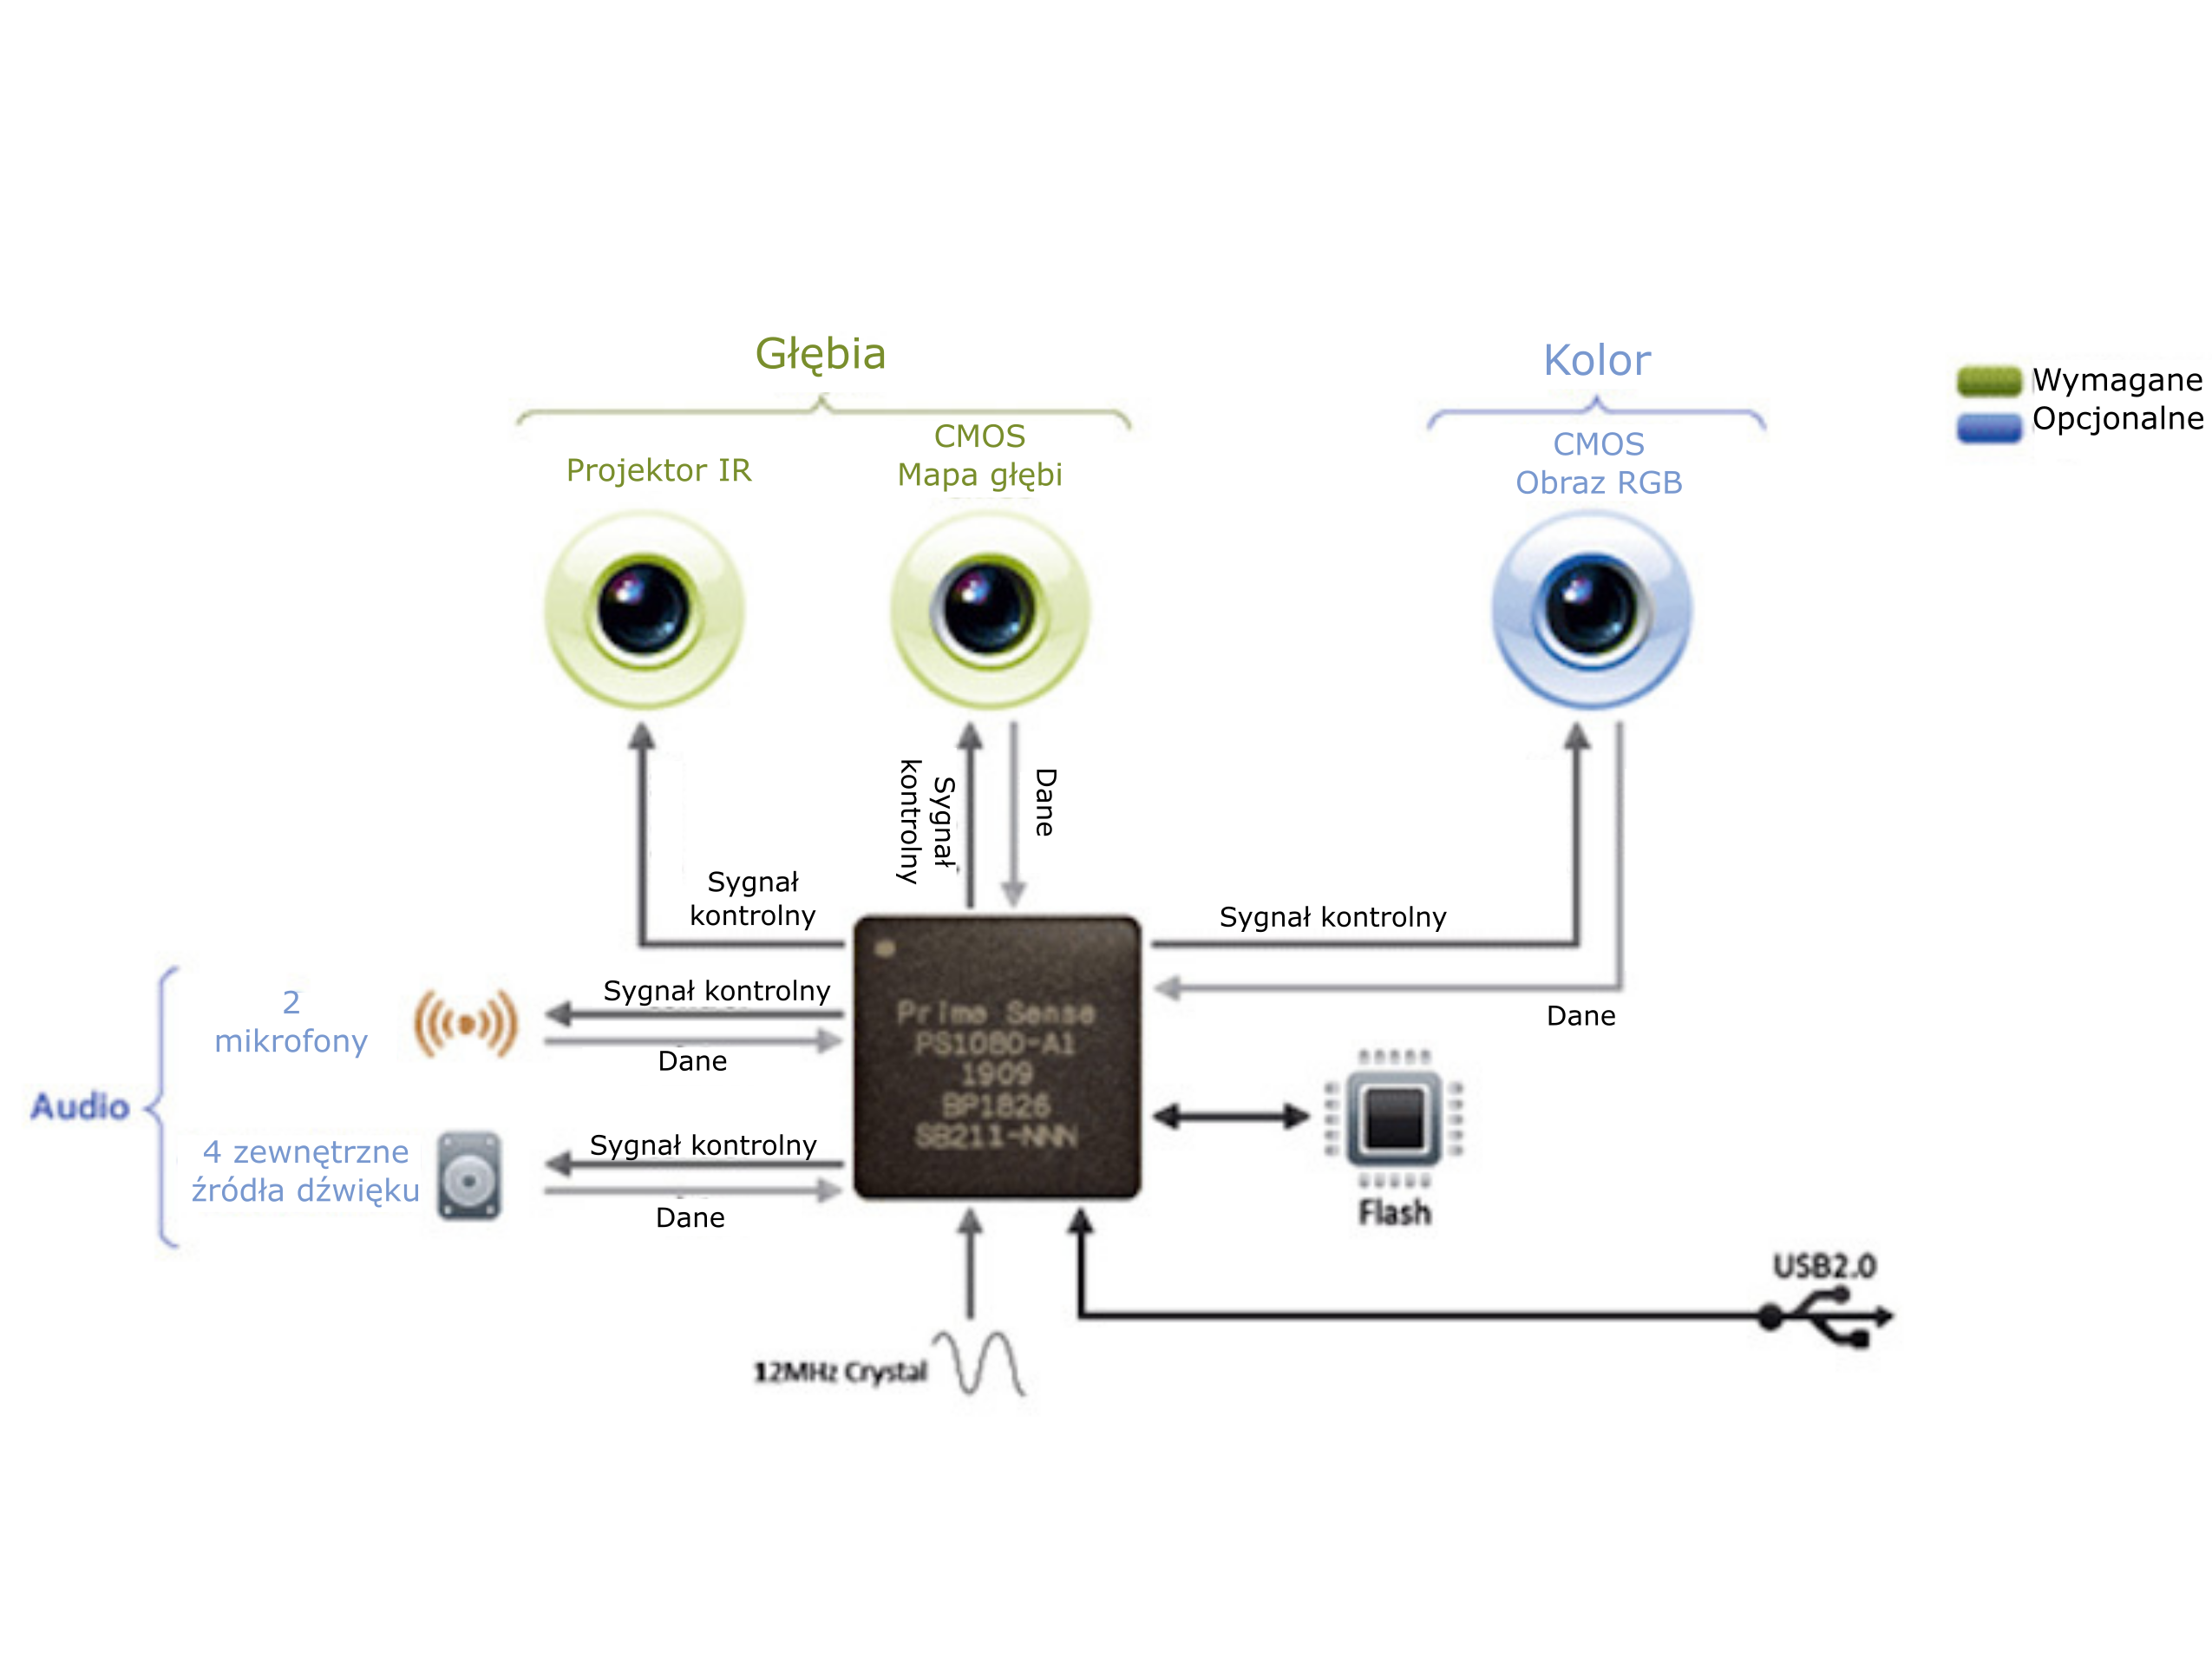
\includegraphics[width=0.95\textwidth]{images/kinectSchema.png}
		\caption[Uproszczony schemat budowy kontrolera Microsoft Kinect v.1]{Uproszczony schemat budowy kontrolera Microsoft Kinect v.1 \footfullcite{footnote:kinectFixit2016}}
		\label{fig:characteristics:kinect:inside} 
	\end{figure}
\end{savenotes}
																															
Według oficjalnej dokumentacji \footfullcite{footnote:kinectSpec2016} Kinect pracuje poprawnie, gdy obiekt (postać) znajduje się w~odległości od $0.8m$ do $4m$ od urządzenia oraz zawiera się w~polu widzenia urządzenia: $57\degree$ w~orientacji poziomej i~$43\degree$ w~orientacji pionowej. Oficjalny zakres pracy urządzenia przedstawia rysunek \ref{fig:characteristics:kinect:range}. Dla odległości mniejszej niż $0.4m$ i~większej niż $8m$ Kinect nie zwraca żadnych wyników pozwalających określić czy jakiś obiekt znajduje się przed nim czy nie. Oficjalna dokumentacja nie zawiera jednak informacji o~ewentualnej niejednorodności precyzji działania w~obszarze pracy urządzenia. Można więc przypuszczać, że urządzenie działa jednakowo precyzyjnie w~dowolnym miejscu znajdującym się w~zakresie roboczym urządzenia \footnote{Eksperymenty badawcze weryfikujące to przypuszczenie zostały zawarte w~dalszej części niniejszego rozdziału \ref{sssection:distanceEstimation}}. Specyfikacja udostępniona na stronach MSDN \footnote{MSDN -- \emph{\textbf{M}icro\textbf{s}oft \textbf{D}eveloper \textbf{N}etwork}, portal internetowy zawierający dokumentacje i~poradniki głównie dla programistów korzystających z~produktów i~narzędzi firmy Microsoft. Dostępny pod adresem \url{http://https://msdn.microsoft.com}} przedstawia prawdopodobnie pewien uśredniony lub minimalny zakres pracy, ponieważ zgodnie z~obserwacjami użytkowników \footfullcite{footnote:stack:kinect2011} oraz badaniami porównawczymi \cite{DiFilippo2015} okazuje się, że poszczególne serie produkcyjne urządzenia mogą mieć nieco inne zakresy pracy. Występowanie różnic w~zakresie działania pomiędzy poszczególnymi egzemplarzami kontrolera Kinect zostało także przewidziane w~oficjalnym SDK przygotowanym przez firmę Microsoft\footfullcite{footnote:msdn:kinectSDKConstants2016}. Analizując kod źródłowy SDK urządzenia można zauważyć rozbieżność pomiędzy dokumentacją dotyczącą maksymalnych zakresów działania, a~faktyczną implementacją. Jako przykład można podać wartość kąta widzenia kamery urządzenia w~pionie, która według dokumentacji wynosi $43\degree$, natomiast faktyczna implementacja podaje różne wartości dla kamer głębi i~RGB, a~wynoszą one odpowiednio $45.6\degree$ i~$48.6\degree$. 
																															
\begin{savenotes}
	\begin{figure}[!htb]
		\centering
		\begin{subfigure}[b]{0.5\textwidth}
			\centering
			
\begin{tikzpicture}[scale=0.4]					
	\draw[very thin,pattern=dots, pattern color = black] (61.5:0.8) -- (61.5:4) arc (61.5:118.5:4) -- (118.5:0.8) arc (118.5:61.5:0.8) -- cycle;						
	\draw[very thin,pattern=horizontal lines, pattern color = black] (61.5:4) -- (61.5:8) arc (61.5:118.5:8) -- (118.5:4) arc (118.5:61.5:4) -- cycle;						
	\draw[very thin,fill=black!10] (61.5:8) -- (61.5:9) arc (61.5:118.5:9) -- (118.5:8) arc (118.5:61.5:8) -- cycle;
																																										
	\draw[dashed, very thin,fill=black!10] (61.5:8) -- (61.5:9) arc (61.5:0:9) -- (0:8) arc (0:61.5:8) -- cycle;
	\draw[dashed, very thin,fill=black!10] (61.5:4) -- (61.5:8) arc (61.5:0:8) -- (0:4) arc (0:61.5:4) -- cycle;
	\draw[dashed, very thin,fill=black!10] (61.5:0.8) -- (61.5:4) arc (61.5:0:4) -- (0:0.8) arc (0:61.5:0.8) -- cycle;
	\draw[dashed, very thin,fill=black!10] (61.5:0.4) -- (61.5:0.8) arc (61.5:0:0.8) -- (0:0.4) arc (0:61.5:0.4) -- cycle;
	\draw[dashed, very thin,fill=black!10] (61.5:0) -- (61.5:0.4) arc (61.5:0:0.4) -- (0:0) arc (0:61.5:0) -- cycle;
																																										
	\draw[dashed, very thin,fill=black!10] (118.5:8) -- (118.5:9) arc (118.5:180:9) -- (180:8) arc (180:118.5:8) -- cycle;
	\draw[dashed, very thin,fill=black!10] (118.5:4) -- (118.5:8) arc (118.5:180:8) -- (180:4) arc (180:118.5:4) -- cycle;
	\draw[dashed, very thin,fill=black!10] (118.5:0.8) -- (118.5:4) arc (118.5:180:4) -- (180:0.8) arc (180:118.5:0.8) -- cycle;
	\draw[dashed, very thin,fill=black!10] (118.5:0.4) -- (118.5:0.8) arc (118.5:180:0.8) -- (180:0.4) arc (180:118.5:0.4) -- cycle;
	\draw[dashed, very thin,fill=black!10] (118.5:0) -- (118.5:0.4) arc (118.5:180:0.4) -- (180:0) arc (180:118.5:0) -- cycle;
																																										
																																										
	\draw[very thin,fill=black!10] (0:0) -- (61.5:0.4) arc (61.5:118.5:0.4) -- (0:0);
																																																							
	\draw[fill=black] (0, 0) circle (0.15);
																																																								
	\draw (0:0.4) node[below right, rotate=-45] {$0.4m$};
	\draw (0:1.2) node[below right, rotate=-45] {$0.8m$};
	\draw (0:4) node[below right, rotate=-45] {$4m$};		
	\draw (0:8) node[below right, rotate=-45] {$8m$};			
	\draw (0:9) node[below right, rotate=-45] {$9m$};
																																																													
	\draw[<->, thin, black] (65:6) arc (65:115:6);
	\draw[black] (80.5: 6) node[above] {$57^\circ$};
																																																						
	\draw (61.5: 9.5) node {$28.5^\circ$};
	\draw (118.5: 9.5) node {$28.5^\circ$};
	\draw[thick, ->] (90:0) -- (90:9.5);
																																																										
	\draw (90: 10) node {Kierunek obserwacji};
\end{tikzpicture}
			\caption{Poziomy zakres pracy}
			\label{fig:kinect:range:a}
		\end{subfigure} \hfill
		\begin{subfigure}[b]{0.5\textwidth}
			\centering
			\begin{tikzpicture}[scale=0.45]
	\draw[very thin,pattern=dots, pattern color = black] (-21.5:0.8) -- (-21.5:4) arc (-21.5:21.5:4) -- (21.5:0.8) arc (21.5:-21.5:0.8) -- cycle;
	\draw[very thin,pattern=horizontal lines, pattern color = black] (-21.5:4) -- (-21.5:8) arc (-21.5:21.5:8) -- (21.5:4) arc (21.5:-21.5:4) -- cycle;
	\draw[very thin,fill=black!10] (-21.5:8) -- (-21.5:9) arc (-21.5:21.5:9) -- (21.5:8) arc (21.5:-21.5:8) -- cycle;
	\draw[very thin,fill=black!10] (-21.5:0) -- (-21.5:0.4) arc (-21.5:21.5:0.4) -- (21.5:0) arc (21.5:-21.5:0) -- cycle;
	\draw[very thin,fill=white] (-21.5:0.4) -- (-21.5:0.8) arc (-21.5:21.5:0.8) -- (21.5:0.4) arc (21.5:-21.5:0.4) -- cycle;
																																																									
	\draw[fill=black] (0, 0) circle (0.15);
	\draw[thick, ->] (0:0) -- (0:9.5);
	\draw (0: 10) node[right] {Kierunek obserwacji};
	% 																																				
	\draw[<->, thin, black] (-18:4.3) arc (-18:18:4.3);
	\draw[black] (-15: 4.3) node[right] {$43^\circ$};
	% 																																				
	\draw[->, thin, black, dashed] (0:6.5) arc (0:-10:6.5);
	\draw[black] (-10: 6.5) node[right] {$-21.5^\circ$};
	% 																																				
	\draw[->, thin, black, dashed] (0:6.5) arc (0:10:6.5);
	\draw[black] (10: 6.5) node[right] {$+21.5^\circ$};
	% 																										
	\draw (0:0) node[left] {Kinect}		;				
	\draw (20.5:0.4) node[above] {$0.4m$};
	\draw (33.5:1.2) node[above] {$0.8m$};
	\draw (21.5:4) node[above] {$4m$};		
	\draw (21.5:8) node[above] {$8m$};			
	\draw (21.5:9) node[above] {$9m$};
																																																									
\end{tikzpicture}
			\caption{Pionowy zakres pracy}
			\label{fig:kinect:range:b}
		\end{subfigure} \hfill
		\begin{subfigure}[p]{\textwidth}
			\hfill
			\begin{tikzpicture}[scale=0.1]	
	\node[draw=black,thick,rounded corners=2pt,below left=2mm] {%
		\begin{tabular}{@{}r@{ }l@{}}
			\raisebox{2pt}{\tikz{\draw[black!10, fill=black!10] (0,0) rectangle (5mm,2mm);}}                               & Niewidoczne                       \\
			\raisebox{2pt}{\tikz{\draw[black,pattern=dots, pattern color = black] (0,0) rectangle (5mm,2mm);}} & Za daleko                         \\
			\raisebox{2pt}{\tikz{\draw[black, fill=black] (0,0) rectangle (5mm,2mm);}}                                     & Za blisko                         \\
			\raisebox{2pt}{\tikz{\draw[black,fill=white] (0,0) rectangle (5mm,2mm);}}             & Obszar roboczy                    \\
			\raisebox{2pt}{\tikz{\draw[<->, thin] (0:0) arc (0:180:0.3);}}                                                 & Zakres pracy                      \\
			\raisebox{2pt}{\tikz{\draw[<-, thin, dashed] (0:0) arc (0:180:0.3);}}                                          & Przesunięcie kierunku obserwacji \\
			\raisebox{2pt}{\tikz{\draw[fill=black] (0, 0) circle (0.15);}}                                                 & Kinect                            
		\end{tabular}};	
\end{tikzpicture}		
               
		\end{subfigure}
																					
		\caption[Poziomy i pionowy zakres pracy kontrolera Microsoft Kinect v.1]{Poziomy (a) i pionowy (b) zakres pracy kontrolera Microsoft Kinect v.1 (na podstawie \footfullcite{footnote:kinectSpec2016})}
		\label{fig:characteristics:kinect:range}	
	\end{figure}
\end{savenotes} 
																															
\subsubsection*{Wyznaczanie mapy głębi}
Sposób w~jaki Kinect określa odległość, w~jakiej umieszczone są przed nim obiekty opiera się o~rozpoznawanie zniekształceń ściśle zdefiniowanego wzorca świetlnego, którym została oświetlona scena (ang. \emph{structured light}). W~tym procesie biorą udział jedynie projektor oraz kamera światła podczerwonego, natomiast obraz z~kamery RGB nie jest wykorzystywany na żadnym etapie określania odległości. Technika ta jest wykorzystywana powszechnie w~skanerach 3D \footfullcite{footnote:david2016} \footfullcite{footnote:lmi2016}. Dokładne działanie kontrolera Kinect nie zostało oficjalnie ujawnione publicznie przez firmę Microsoft. Możliwe jest jednakże przedstawienie przybliżonego działania tego kontrolera dzięki niezależnym badaniom (np.: MacCormick \cite{MacCormick2011}) oraz analizie zgłoszeń patentowych \cite{patent:20080106746,patent:20100020078,patent:20100118123} należących do producenta procesora wykorzystanego do budowy kontrolera Kinect -- firmy Prime Sense.
																															
W pierwszym kroku cała scena zostaje oświetlona zbiorem punktów za pomocą projektora światła podczerwonego (rys. \ref{fig:characteristics:kinect:nightVision}) zgodnie ze ściśle określonym wzorcem (rys. \ref{fig:characteristics:kinect:dotPattern}). Wzorzec ten nie został nigdy oficjalnie opublikowany przez firmy Prime Sense, czy Microsoft, natomiast wzorzec zamieszczony na rysunku \ref{fig:characteristics:kinect:dotPattern} został wyznaczony przez Andreasa Reichingera, doktoranta na Uniwersytecie Technicznym w~Wiedniu. Na swoim blogu opublikował on dokładny opis sposobu wyznaczania zamieszczonego wzorca\footfullcite{footnote:reichinger2011}.
																															
\begin{savenotes}
	\begin{figure}[!htb]
		\centering
		\begin{minipage}[b]{0.48\linewidth}
			\centering   
			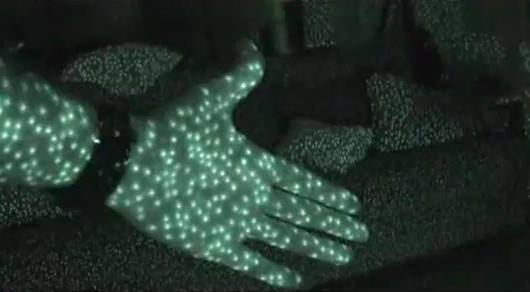
\includegraphics[width=\textwidth]{images/kinectNightVision.jpg}	
			\caption[Scena oświetlona promieniami podczerwonymi]{Scena oświetlona promieniami IR\footfullcite{footnote:flatley2011}}
			\label{fig:characteristics:kinect:nightVision}
		\end{minipage}
		\hfill
		\begin{minipage}[b]{0.48\linewidth}
			\centering 
			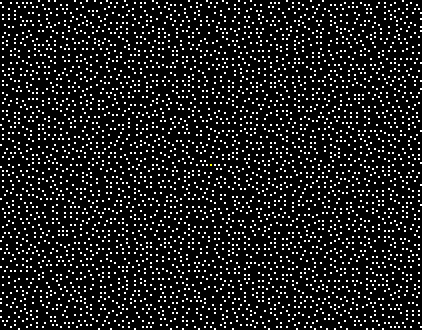
\includegraphics[width=\textwidth]{images/kinect-pattern_3x3.png}
			\caption[Wzorzec oświetlenia sceny przez kontroler Kinect]{Wzorzec oświetlenia sceny przez kontroler Kinect \footfullcite{footnote:reichinger2011}}
			\label{fig:characteristics:kinect:dotPattern}
		\end{minipage}	
	\end{figure}
\end{savenotes}
																																	
Pełen wzorzec zbudowany jest z~9 powtarzających się regionów w~układzie 3x3 o~rozmiarze 211x165 punktów, co daje pełen rozmiar wzorca równy 633x495 punktów. Około $11\%$ z~tych punktów jest jasna, przy czym jasność ta nie jest jednorodna. Wyraźnie można zauważyć, że część punktów jest jaśniejsza od pozostałych. Ponadto w~punkcie centralnym każdego z~regionów (jak i~całego wzorca) znajduje się najjaśniejszy z~punktów. Dodatkowo wzorzec ten jest skośnie symetryczny, co oznacza niewrażliwość na obrócenie urządzenia~o~$180\degree$.
																																	
Następnym krokiem jest wyznaczenie mapy głębi na podstawie analizy zniekształcenia wyświetlonego wzorca. Opierając się na badaniach prowadzonych przez MacCormicka \cite{MacCormick2011}, analiza zniekształcenia wzorca opiera się na dwóch technikach:
																																	
\begin{itemize}
	\item wyznaczenie głębi na podstawie ostrości punktów,
	\item wyznaczenie głębi na podstawie zjawiska paralaksy.
\end{itemize}
																																	
Pierwsza z~technik opiera się na fakcie, że obraz obiektów umieszczonych bliżej soczewki jest mniej wyostrzony od tych znajdujących się dalej. Dodatkowo soczewki umieszczone w~kamerze IR Kinecta posiadają różną ogniskową dla osi ''X'' i~''Y'', co sprawia, że okrągłe punkty stają się eliptyczne z~pochyleniem zależnym od głębokości w~jakiej znajduje się dany obiekt. Druga z~zastosowanych technik opiera się na zjawisku paralaksy, które występuje w~wyniku przesunięcia pomiędzy projektorem światła podczerwonego, a~kamerą wyposażoną w~filtr światła o~częstotliwości z zakresu podczerwonego. Szczegółowe opisy działania obu technik można znaleźć w~wielu publikacjach naukowych m.in.: Rzeszotarski, Strumiłło i in. \cite{Rzeszotarski2006}, czy Fofi, Sliwa, Voisin \cite{Fofi2004}. Informacje uzyskane na podstawie obu powyższych technik są następnie ze sobą łączone w~celu uzyskania mapy głębi.
																																	
\subsubsection*{Ograniczenia w~działaniu kontrolera Kinect}\label{ssec:characteristics:kinect:limitation}
																																	
Kinect przez ponad 5 lat dostępności na rynku jest obiektem badań związanych zarówno z~jego zastosowaniem i~poprawą działania, jak i~dokładnym opisaniem jego cech, oszacowaniu dokładności oraz zdefiniowaniu ograniczeń. Jednym z~podstawowych ograniczeń jakie występują w~tym urządzeniu jest wrażliwość na światło słoneczne. Jak to zostało wcześniej opisane, jedynym źródłem danych wykorzystywanym do budowy mapy głębi, a~także do stworzenia modelu szkieletowego jest kamera z~filtrem podczerwieni oraz wzorzec punktów podczerwonych emitowanych przez wbudowany projektor. Światło słoneczne natomiast składa się z~pełnego spektrum barw, zarówno z~zakresu widzialnego jak i~niewidzialnego dla człowieka. Oznacza to, że promienie słoneczne mogą wprowadzić dodatkowe punkty na scenie, które nie należą do wzorca, a~będą zarejestrowane przez kamerę. Zarejestrowanie przez kamerę podczerwoną kontrolera Kinect punktów spoza przyjętego wzorca prowadzi do niepoprawnego zbudowania mapy głębi wykorzystywanej w~procesie wyznaczania modelu szkieletowego. Rysunek \ref{fig:characteristics:kinect:depthMap} przedstawia mapę głębi zbudowaną wewnątrz pomieszczenia \ref{fig:characteristics:kinect:depthMapA} oraz na zewnątrz w~dwóch przypadkach, w~miejscu zacienionym \ref{fig:characteristics:kinect:depthMapB} oraz w~pełnym słońcu \ref{fig:characteristics:kinect:depthMapC}. 
																																	
\begin{savenotes}
	\begin{figure}[!htb]
		\captionsetup{singlelinecheck=off}
		\centering
		\begin{subfigure}[b]{0.3\textwidth}
			\centering
			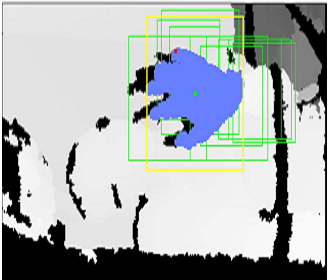
\includegraphics[width=\textwidth]{images/kinectIndoor.png}	
			\caption{Wewnątrz pomieszczenia}
			\label{fig:characteristics:kinect:depthMapA}
		\end{subfigure}
		\hfill																																				
		\begin{subfigure}[b]{0.3\textwidth}
			\centering
			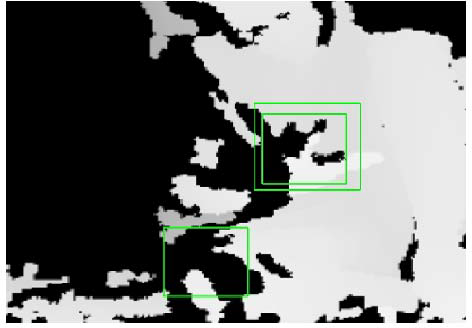
\includegraphics[width=\textwidth]{images/kinecOutdoorShade.png}		
			\caption{Na zewnątrz pomieszczenia w~cieniu}
			\label{fig:characteristics:kinect:depthMapB}
		\end{subfigure}
		\hfill																																
		\begin{subfigure}[b]{0.3\textwidth}
			\centering
			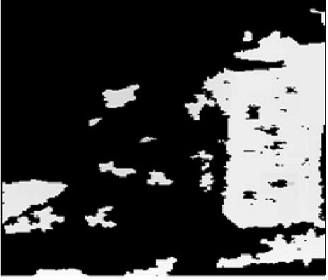
\includegraphics[width=\textwidth]{images/kinecOutdoorFull.png}		
			\caption{Na zewnątrz pomieszczenia w~świetle słonecznym}
			\label{fig:characteristics:kinect:depthMapC}
		\end{subfigure}
																																																	
		\caption[Mapa głębi ręki w~różnych warunkach oświetleniowych]{Mapa głębi ręki w~różnych warunkach oświetleniowych\cite{Suarez2012}.}
		\label{fig:characteristics:kinect:depthMap}
	\end{figure}
\end{savenotes}
																																	
																																			
Jak widać na przykładzie z~rysunku \ref{fig:characteristics:kinect:depthMap}, Kinect nie był w~stanie zbudować prawidłowej mapy w~przypadku oświetlenia sceny światłem słonecznym. \\
Z podobnych względów niezalecane jest używanie wielu Kinectów do śledzenia ruchu na jednej scenie. Co prawda SDK wspiera wykorzystanie aż 4 urządzeń równocześnie, jednak zgodnie z~oficjalną dokumentacją może to negatywnie wpłynąć na dokładność rozpoznawania części ciała, a~przez to wyznaczenia modelu szkieletowego i~śledzenia ruchu stawów \footfullcite{footnote:msdn:multipleKinectsSDK2016}. Należy jednak wspomnieć, że scenariusz wykorzystania wielu kontrolerów Microsoft Kinect w~przypadku jednej sceny, jest jednym z~obszarów badawczych wśród naukowców. Po zastosowaniu odpowiednich algorytmów wspomagających proces kalibracji i~synchronizacji \cite{Kohno2013}, czy wprowadzających elementy uczenia maszynowego (rozpoznawanie szkieletu z~wykorzystaniem klasyfikator HCRF - ang. \emph{Hidden-state Conditional Random Fields }) \cite{Kitsikidis2011}, badacze osiągneli możliwość stabilnej pracy układu kilku kontrolerów Kinect z dokładnością wyższą niż w przypadku pojedynczego kontrolera. Badając możliwości wykorzystania kilku kontrolerów Kinect do obserwacji jednej sceny badacze byli w~stanie także poprawić działanie systemu śledzenia z~wykorzystaniem jednego urządzenia. Przykładowo, Asteriadis \cite{Asteriadis2013} oraz Baek \cite{Baek2014} opisali metody wykorzystania dwóch kontrolerów Kinect, dzięki którym zmniejszyli oni podatność prezentowanego systemu śledzenia na występowanie okluzji, a~przez to tracenia możliwości śledzenia ruchu stawów. To z~kolei przekłada się na dokładność oszacowania położenia stawów. Shroeder \cite{Schroder2011} zaproponował natomiast metodę poprawiającą jakość wyznaczonej mapy głębi. Według opublikowanych danych zminiejszył on liczbę pikseli niepoprawnie określających głębię z~około $20\%$ do $1\%$.


%%%%%%%%%%%%%%%%%%%%%%%%%%%%%%%%%%%%%%%%%5
Kontroler microsoft Kinect, na podstawie swoich pomiarów, estymuje trójwymiarowy model szkieletowy śledzonej postaci, w którym pozycja każdego stawu opisana jest przez trójkę liczb pozwalającą określić jednoznacznie położenie tego stawu. Twórcy tego urządzenia przyjeli, że z~każdym stawem powiązany jest tylko jeden punkt w~przestrzeni i jest on powiązany ze swoim sąsiednim stawem definiując w ten sposób kość. Mając udostępnioną informację o położeniu w przestrzeni dwós sąsiednich stawów, możemy wyznaczyć 


jesteśmy w~stanie określić kierunek obrotu danej kości jednak jest to informacja ograniczona jedynie do dwóch wymiarów wyłączając obrót wokół własnej osi. 

Układ współrzędnych kontrolera Kinect zakłada, że jego początkiem (punkt $(0, 0, 0)$) jest kontroler, a~wszystkie udostępnione przez niego pomiary są pomiarami względnymi w~stosunku do niego samego. 

Innym ograniczeniem, jakie należy wziąć pod uwagę, jest zasłanianie stawów śledzonej postaci. Okluzja może wystąpić z~dwóch powodów:
\begin{itemize}
	\item przysłonięcie przez obiekty znajdujące się na scenie na przykład meble,
	\item przysłonięcie przez inne części ciała.
\end{itemize}
																																			
W tym miejscu należy wspomnieć o~informacji przypisanej do każdego ze stawów określającej stan jego śledzenia. Informacja ta może przyjąć jedną z~3 wartości:
\begin{itemize}
	\item \emph{Tracked} -- wartość przyjmowana kiedy dany staw jest w~pełni widoczny i~śledzony bez żadnych znaczących zakłóceń;
	\item \emph{Interferred} -- wartość przyjmowana kiedy Kinect nie jest w~stanie śledzić danego stawu, ale na podstawie innych wartości jest w~stanie oszacować jego położenie. Algorytm jakim w~tej sytuacji posługuje się Kinect do szacowania położenia nie został opublikowany;
	\item \emph{NotTracked} -- wartość przyjmowana kiedy dany staw jest zupełnie niewidoczny i~nie ma możliwości podania nawet jego przybliżonego położenia;
\end{itemize}
																																			
W praktyce, położenie stawów jest najczęściej oznaczone jako \emph{Interferred}, co oznacza, że należy dodatkowo weryfikować otrzymane dane zanim zostaną użyte, przykładowo, czy położenie danego stawu pomiędzy kolejnymi pomiarami jest prawdopodobne, lub wystąpił jednak błąd szacowania. Sposobem na taką weryfikację może być wyznaczenie stopnia przesunięcia danego stawu pomiędzy kolejnymi pomiarami. Przy częstotliwości akwizycji danych przez kontroler Kinect, która wynosi 30 klatek na sekundę, czas jaki mija pomiędzy dwiema kolejnymi klatkami to około 30ms. Tak krótki czas sprawia, że przesunięcia stawów przy normalnym ruchu postaci są realnie niewielkie. Jeśli zatem wyznaczone przesunięcie będzie wynosiło przykładowo 1 metr, istnieje duże prawdopodobieństwo, że położenie stawu zostało oszacowane błędnie.
																																			
Szczególne przypadki okluzji występują, gdy użytkownik skieruje wyprostowaną kończynę w~kierunku kamery Kinecta lub obróci się cała jego sylwetka względem płaszczyzny obserwacji kontrolera Kinect. Analizując pierwszy scenariusz najłatwiej przedstawić go na przykładzie ruchu ręki. Trzymając ją na wprost kamery kontrolera Kinect, wyprostowaną w~łokciu, w~pełni widoczny jest tylko staw nadgarstkowy, a~także dłoń. Praktycznie całkowitemu przysłonięciu ulegają zaś łokieć i~staw barkowy. 
																																			
\begin{savenotes}
	\begin{figure}[!htb]
		\centering
		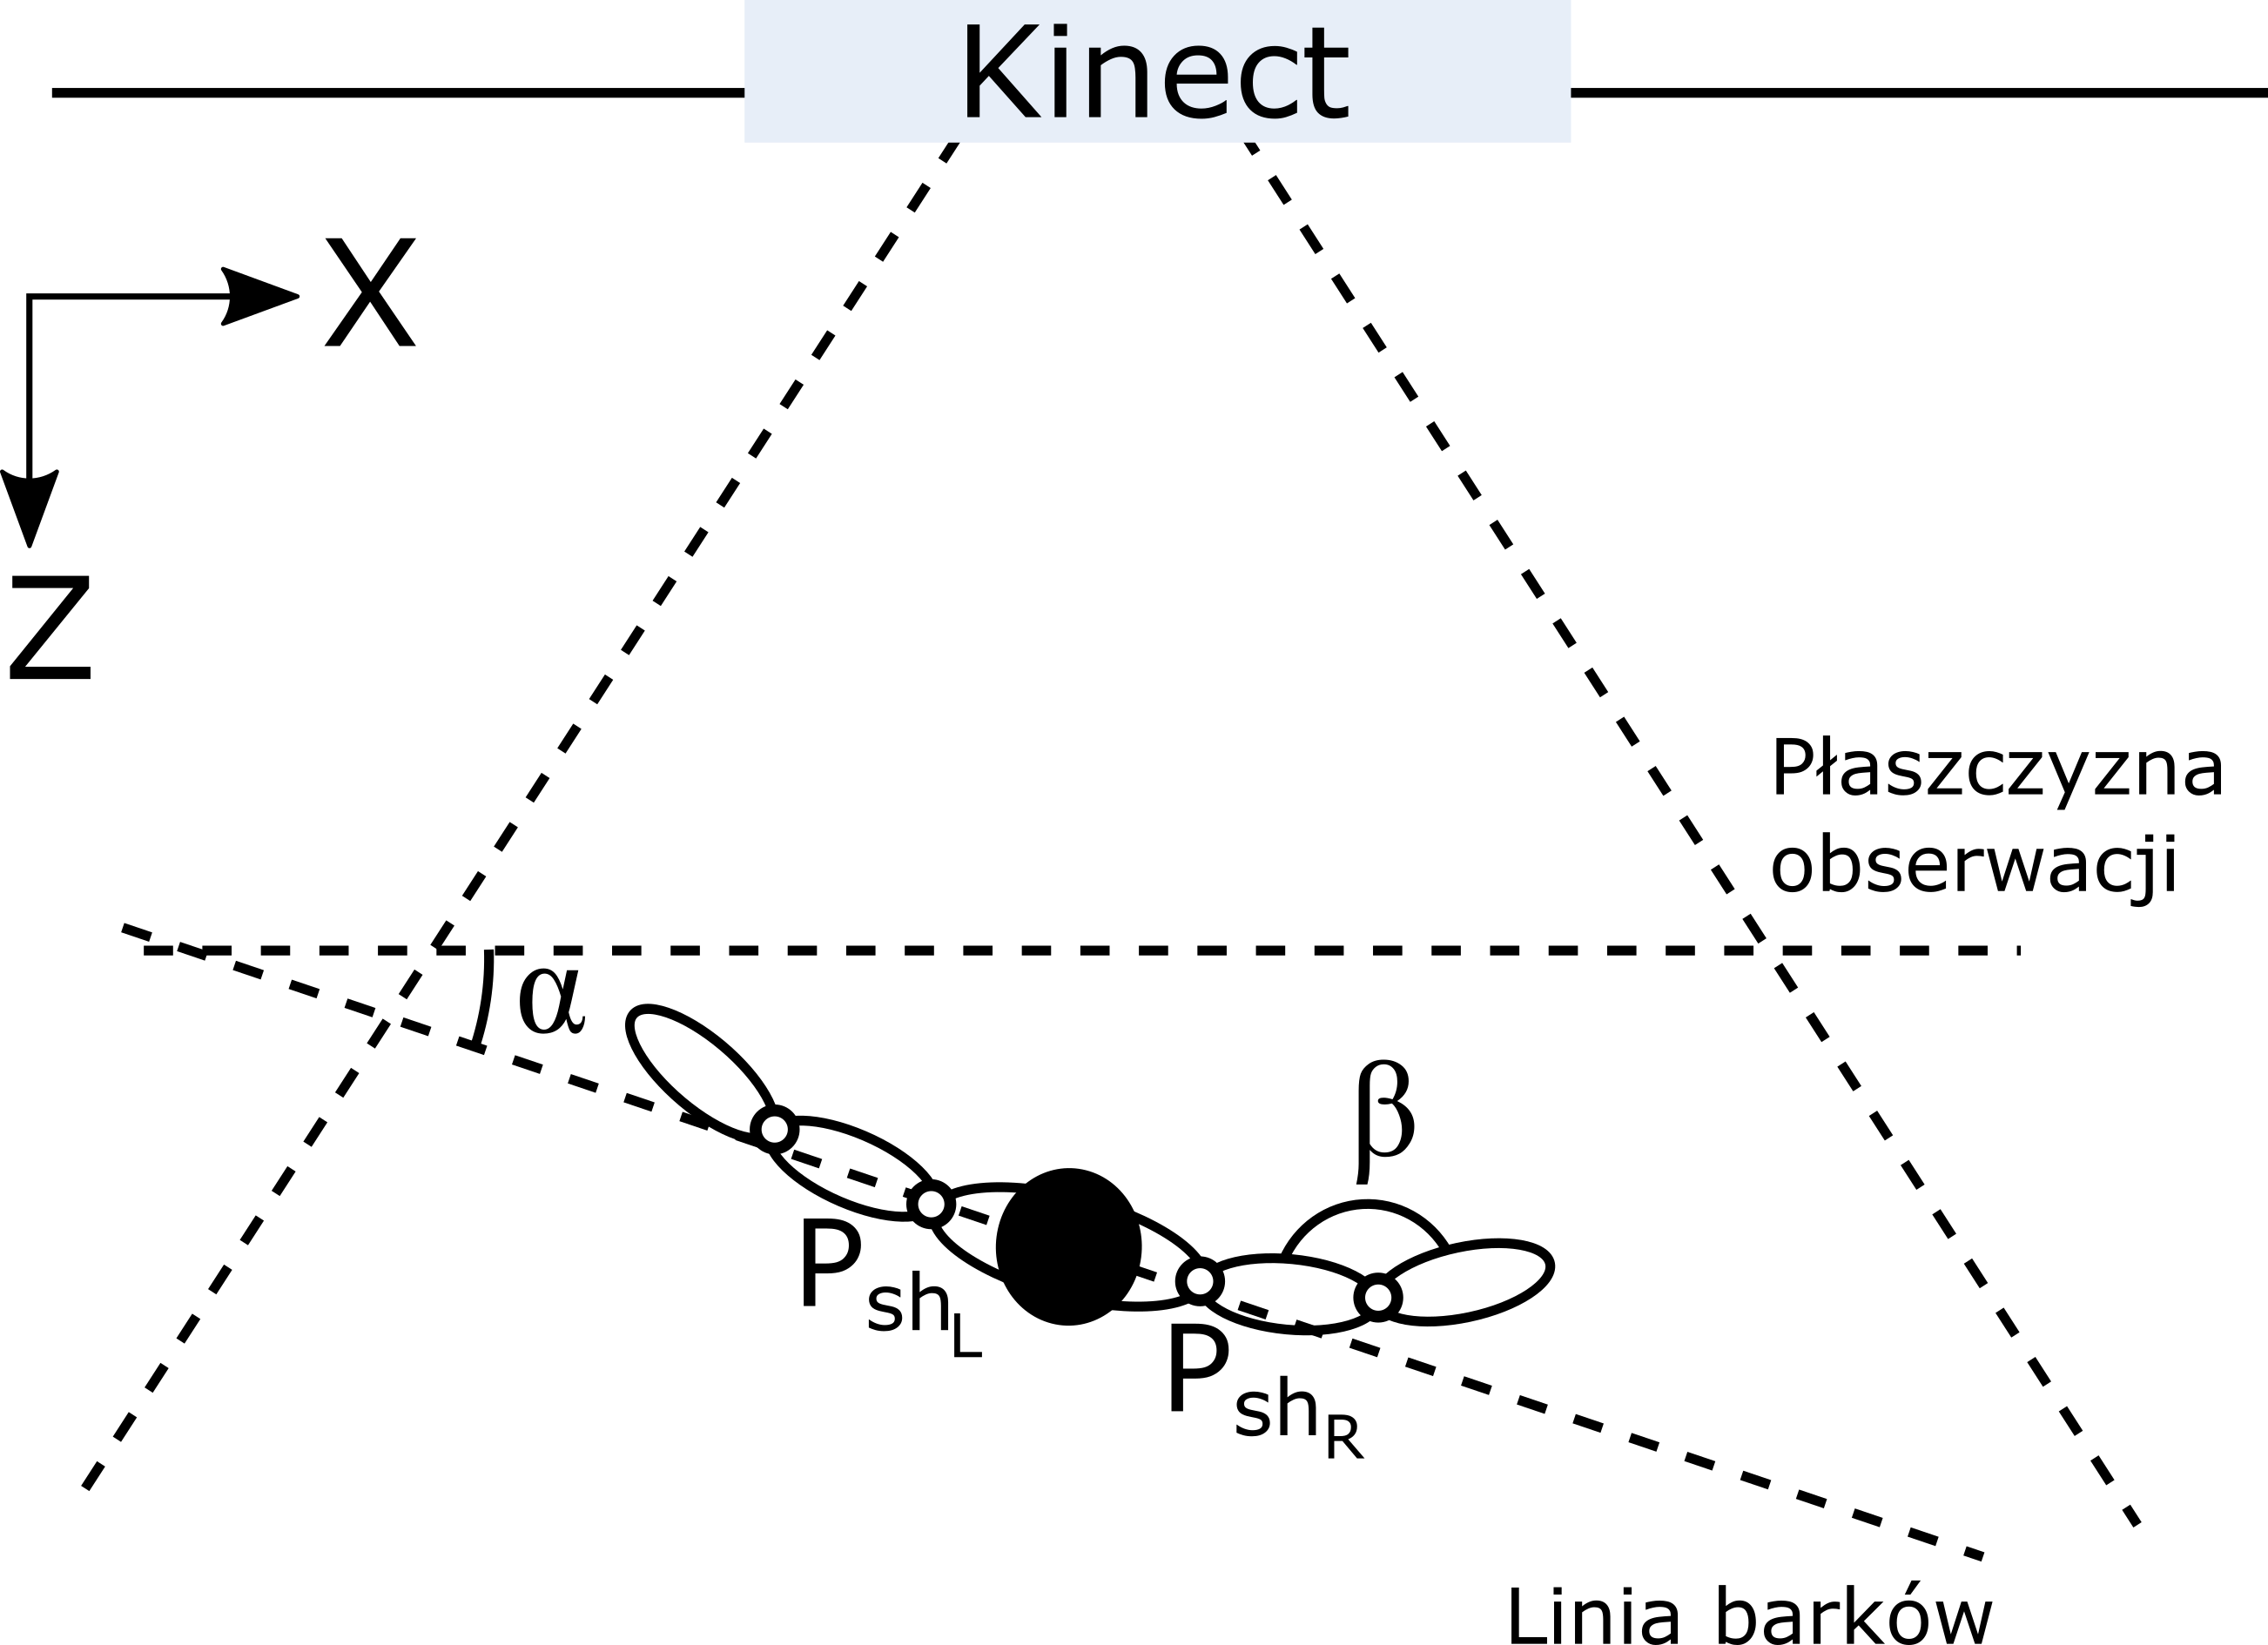
\includegraphics[width=0.5\textwidth]{images/kinectAngle.png}
		\caption{Kąt obrotu użytkownika względem Kinecta}
		\label{fig:characteristics:kinect:bodyRotationAngle}
	\end{figure}
\end{savenotes}
																																					
W trakcie badań własnych przeprowadzony został eksperyment, którego celem było oszacowanie przy jakim kącie obrotu ciała śledzonej postaci względem kontrolera Kinect następuje praktyczna utrata zdolności śledzenia wybranych stawów przez kontroler. Eksperyment polegał na obracaniu się postaci wokół własnej osi w~tak zwanej pozycji \emph{T--pose}, co oznacza, obie ręce wyprostowane w~łokciach i~wyciągnięte w~bok, tak że sylwetka przypomina literę "`T"'. W~trakcie wykonywania ruchu mierzony był kąt obrotu $\alpha$ pomiędzy linią barków ($P_{{Sh}_L, P_{{Sh}_R}}$), a~płaszczyzną obserwacji (rys. \ref{fig:characteristics:kinect:bodyRotationAngle}). Kąt ten jest wyznaczony w~przestrzeni dwuwymiarowej i~wyrażony jest wzorem \ref{eq:characteristics:kinect:bodyRotationAngle}. Wszystkie współrzędne użyte w~tym wzorze wyrażone są w~układzie współrzędnych Kinecta (rys. \ref{fig:characteristics:kinect:space}).
																																			
\begin{equation}
	\label{eq:characteristics:kinect:bodyRotationAngle}
	\begin{split}
		\alpha &= 
		\begin{cases} 
			atan(\frac{|p^K_{{Sh}_R,Z} - p^K_{{Sh}_L,Z}|}{|p^K_{{Sh}_R,X} - p^K_{{Sh}_L,X}|} & , |p^K_{{Sh}_R,X} - p^K_{{Sh}_L,X}| \neq 0 \\
			\frac{\Pi}{2}                                                                    & , |p^K_{{Sh}_R,X} - p^K_{{Sh}_L,X}| = 0    \\		
		\end{cases}
	\end{split}
\end{equation}
gdzie:
\begin{conditions}
	p^K_{{Sh}_L,X}, p^K_{{Sh}_L,Z}			& współrzędne pobrane z~kontrolera Kinect określające położenie lewego barku użytkownika w~osiach X i~Z,\\
	p^K_{{Sh}_R,X}, p^K_{{Sh}_R,Z}			& współrzędne pobrane z~kontrolera Kinect określające położenie prawego barku użytkownika w~osiach X i~Z.\\
\end{conditions}
																																					
																																					
W wyniku eksperymentu okazało się, że przy kącie obrotu $\alpha$ powyżej $50\degree$ kontroler Kinect traci z~pola widzenia blisko połowę stawów użytkownika, a~to z~kolei powoduje, że pomiar wszystkich pozostałych stawów staje się niewiarygodny. Objawia się to dużymi różnicami w~oszacowaniu pozycji stawów pomiędzy dwoma kolejnymi pomiarami. Co ciekawe, różnice te są także zauważalne dla stawów oznaczonych jako \emph{Tracked}, czyli teoretycznie takich, które są w~pełni widoczne dla kontrolera. Na tej podstawie można wysunąć dwa wnioski. Po pierwsze wyznaczenie pozycji poszczególnych stawów odbywa się z~wykorzystaniem informacji o~pozostałych stawach. W~innym przypadku stawy oznaczone jako \emph{Tracked} zawsze byłyby pozycjonowane w~poprawny sposób. Drugi wniosek jaki się nasuwa dotyczy póz wykorzystywanych jako zestaw uczący dla algorytmu losowych lasów decyzyjnych (rozdział \ref{chap:humanModel:kinect}). Pozy wykorzystywane do nauczenia Kinecta prawidłowego rozpoznawania części ciała człowieka przedstawiają prawdopodobnie postać stojącą na wprost, względnie obruconą w~niewielkim stopniu do płaszczyzny obserwacji. Stąd problemy kontrolera Kinect w~określaniu położenia nawet widocznych stawów w~sytuacji, gdy śledzona postać jest obrócona.
																																					
Wykres na rysunku \ref{fig:characteristics:kinect:bodyRotationChart} przedstawia status śledzenia lewego i~prawego barku (linie przerywane) w~zależności od kąta obrotu $\alpha$ wyznaczonego na podstawie pomiarów Kinecta (linia ciągła). Stan śledzenia stawu \emph{Tracked} reprezentowany jest przez wartość liczbową $1$ (wartość na prawej osi pionowej) natomiast stan \emph{Interferred} przez wartość $0.5$. Obrót wykonywany był w~kierunku przeciwnym do ruchu wskazówek zegara co oznacza, że prawa strona ciała była cały czas widoczna dla urządzenia śledzącego ruch. Jak widać na tym wykresie, przy kącie zbliżonym do $50\degree$ status śledzenia zaczyna zmieniać się gwałtownie, aby ustalić swoją wartość po przekroczeniu rzeczonego kąta. W~przedziale od $50\degree$ do $90\degree$ można zaobserwować duże wahania pomiaru, co jest spowodowane błędnym szacowaniem położenia lewego barku.\\ 
Wykres przedstawiony na rysunku \ref{fig:characteristics:kinect:kinectRightHandElbowAngle} pokazuje również zmianę wartości kąta mierzonego w~łokciu prawej ręki $\beta$ (rys. \ref{fig:characteristics:kinect:bodyRotationAngle}) w~trakcie wykonywania obrotu. Ręka przez cały czas trwania obrotu była wyprostowana w~łokciu i~stanowiła przedłużenie linii pomiędzy barkami (\emph{T--pose}). Jak widać na wykresie, pomimo pełnej widoczności prawej ręki przez kamery Kinecta przy obrocie w~zakresie  $50\degree < \alpha \le 90\degree$ , pomiar kąta $\beta$ jest niestabilny, a~jego wartość nie jest nawet zbliżona do wartości kąta wyprostowanej w~łokciu ręki ($170\degree-180\degree$). 
																																							
\begin{savenotes}
	\begin{figure}[!htb]
		\captionsetup{singlelinecheck=off}
		\centering
		\begin{subfigure}[b]{0.8\textwidth}
			\centering
			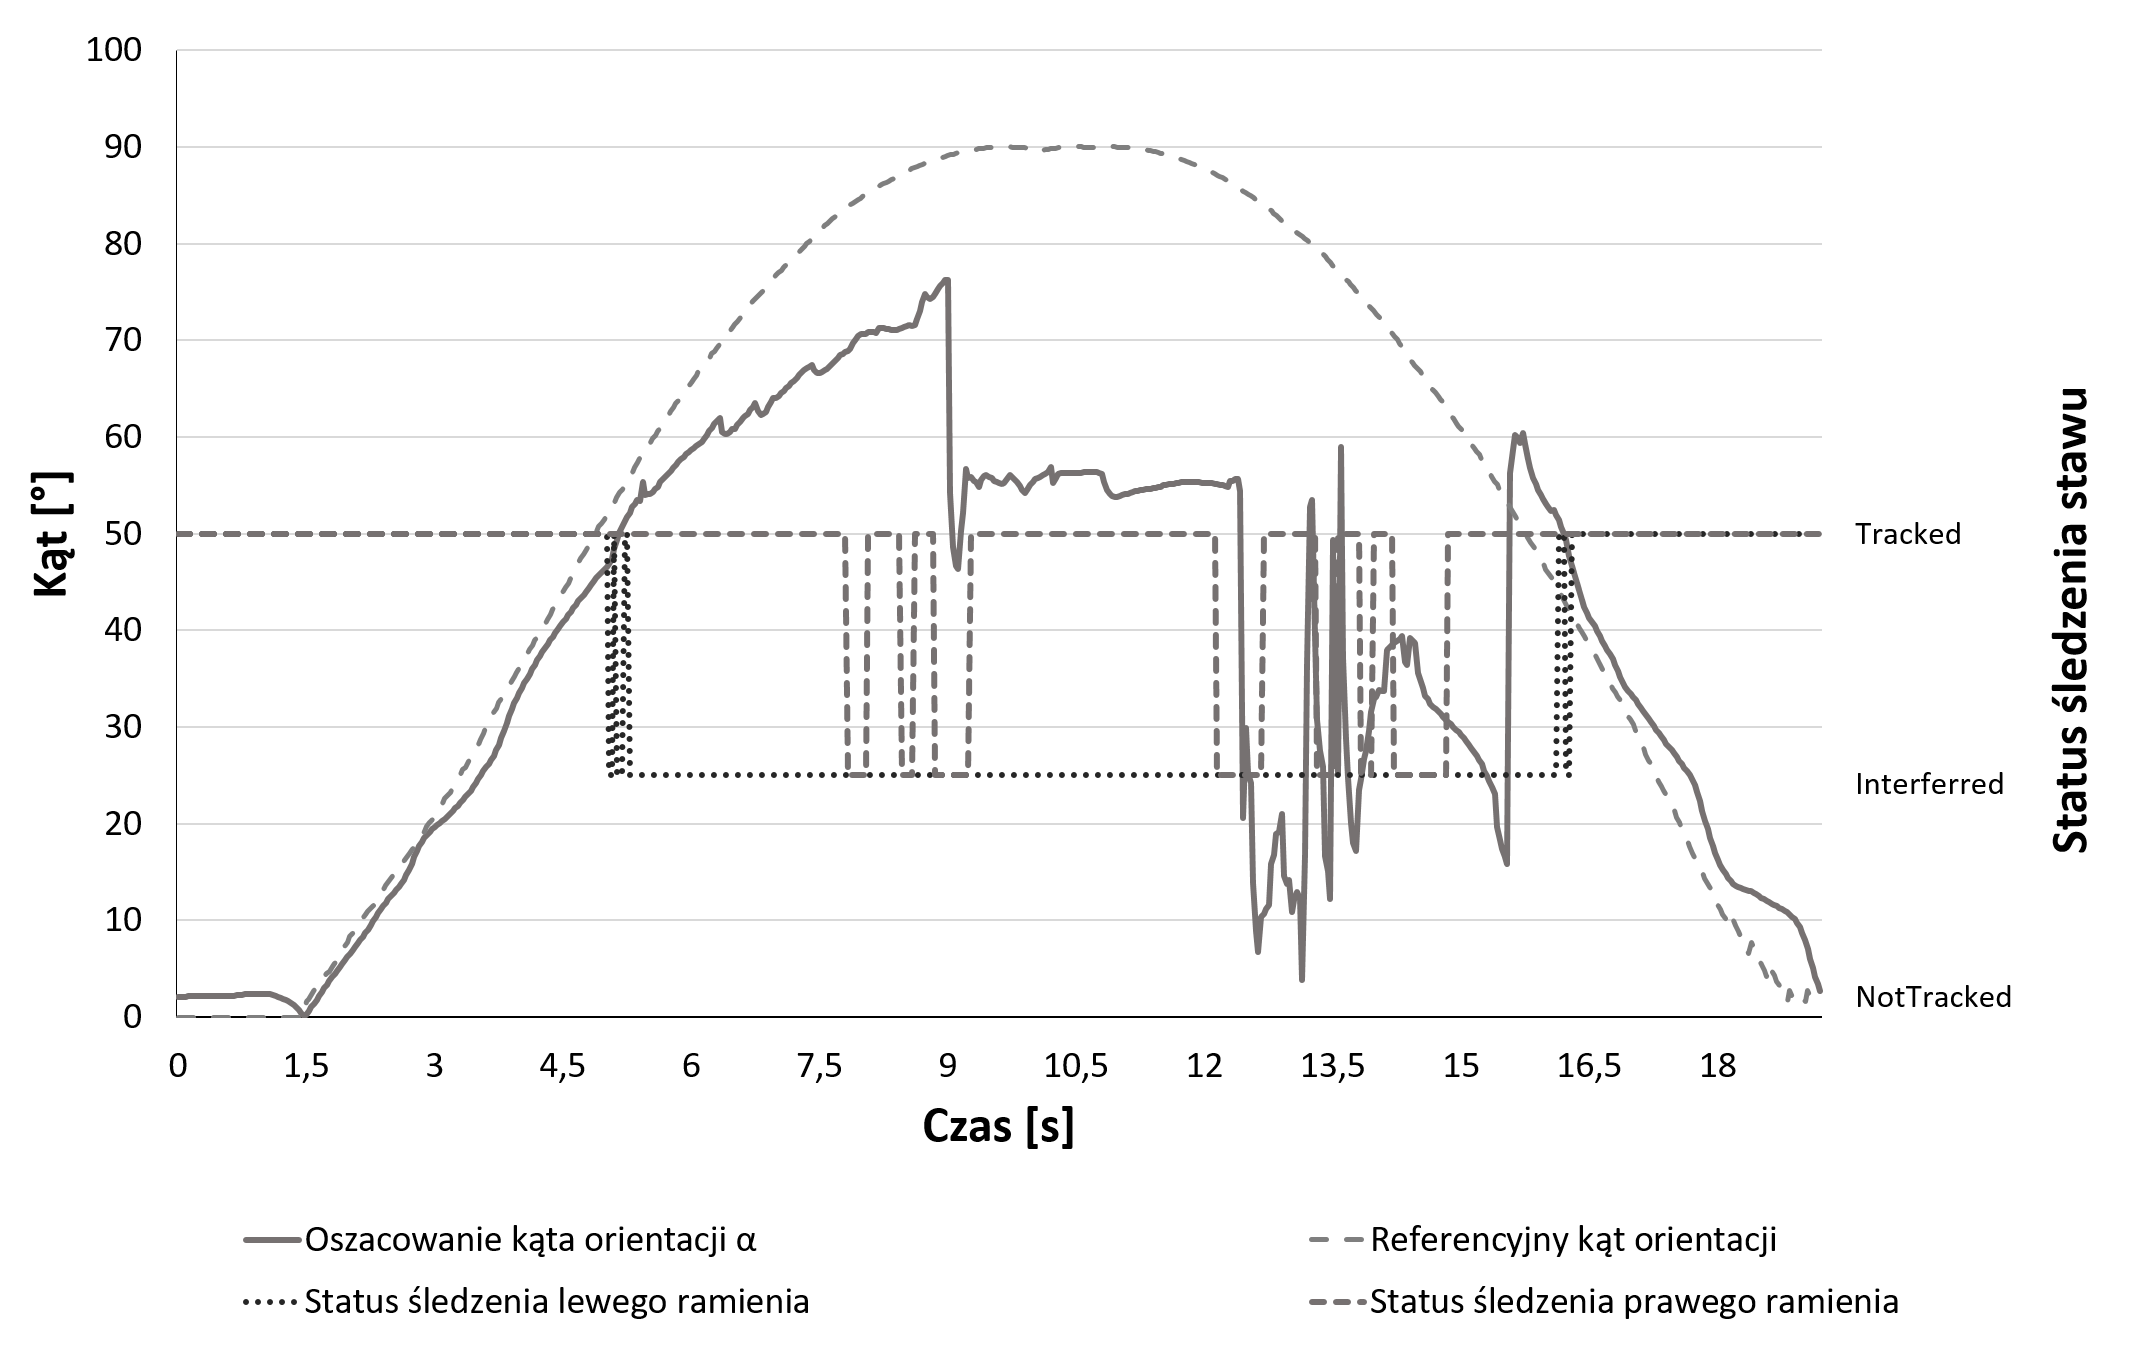
\includegraphics[width=\linewidth]{images/kinectRotation.png}	
			\caption{Stan śledzenia stawów podczas obrotu ciała \emph{(T-pose)} względem kontrolera}
			\label{fig:characteristics:kinect:bodyRotationChart}
		\end{subfigure}
																																																						
		\begin{subfigure}[b]{0.8\textwidth}
			\centering
			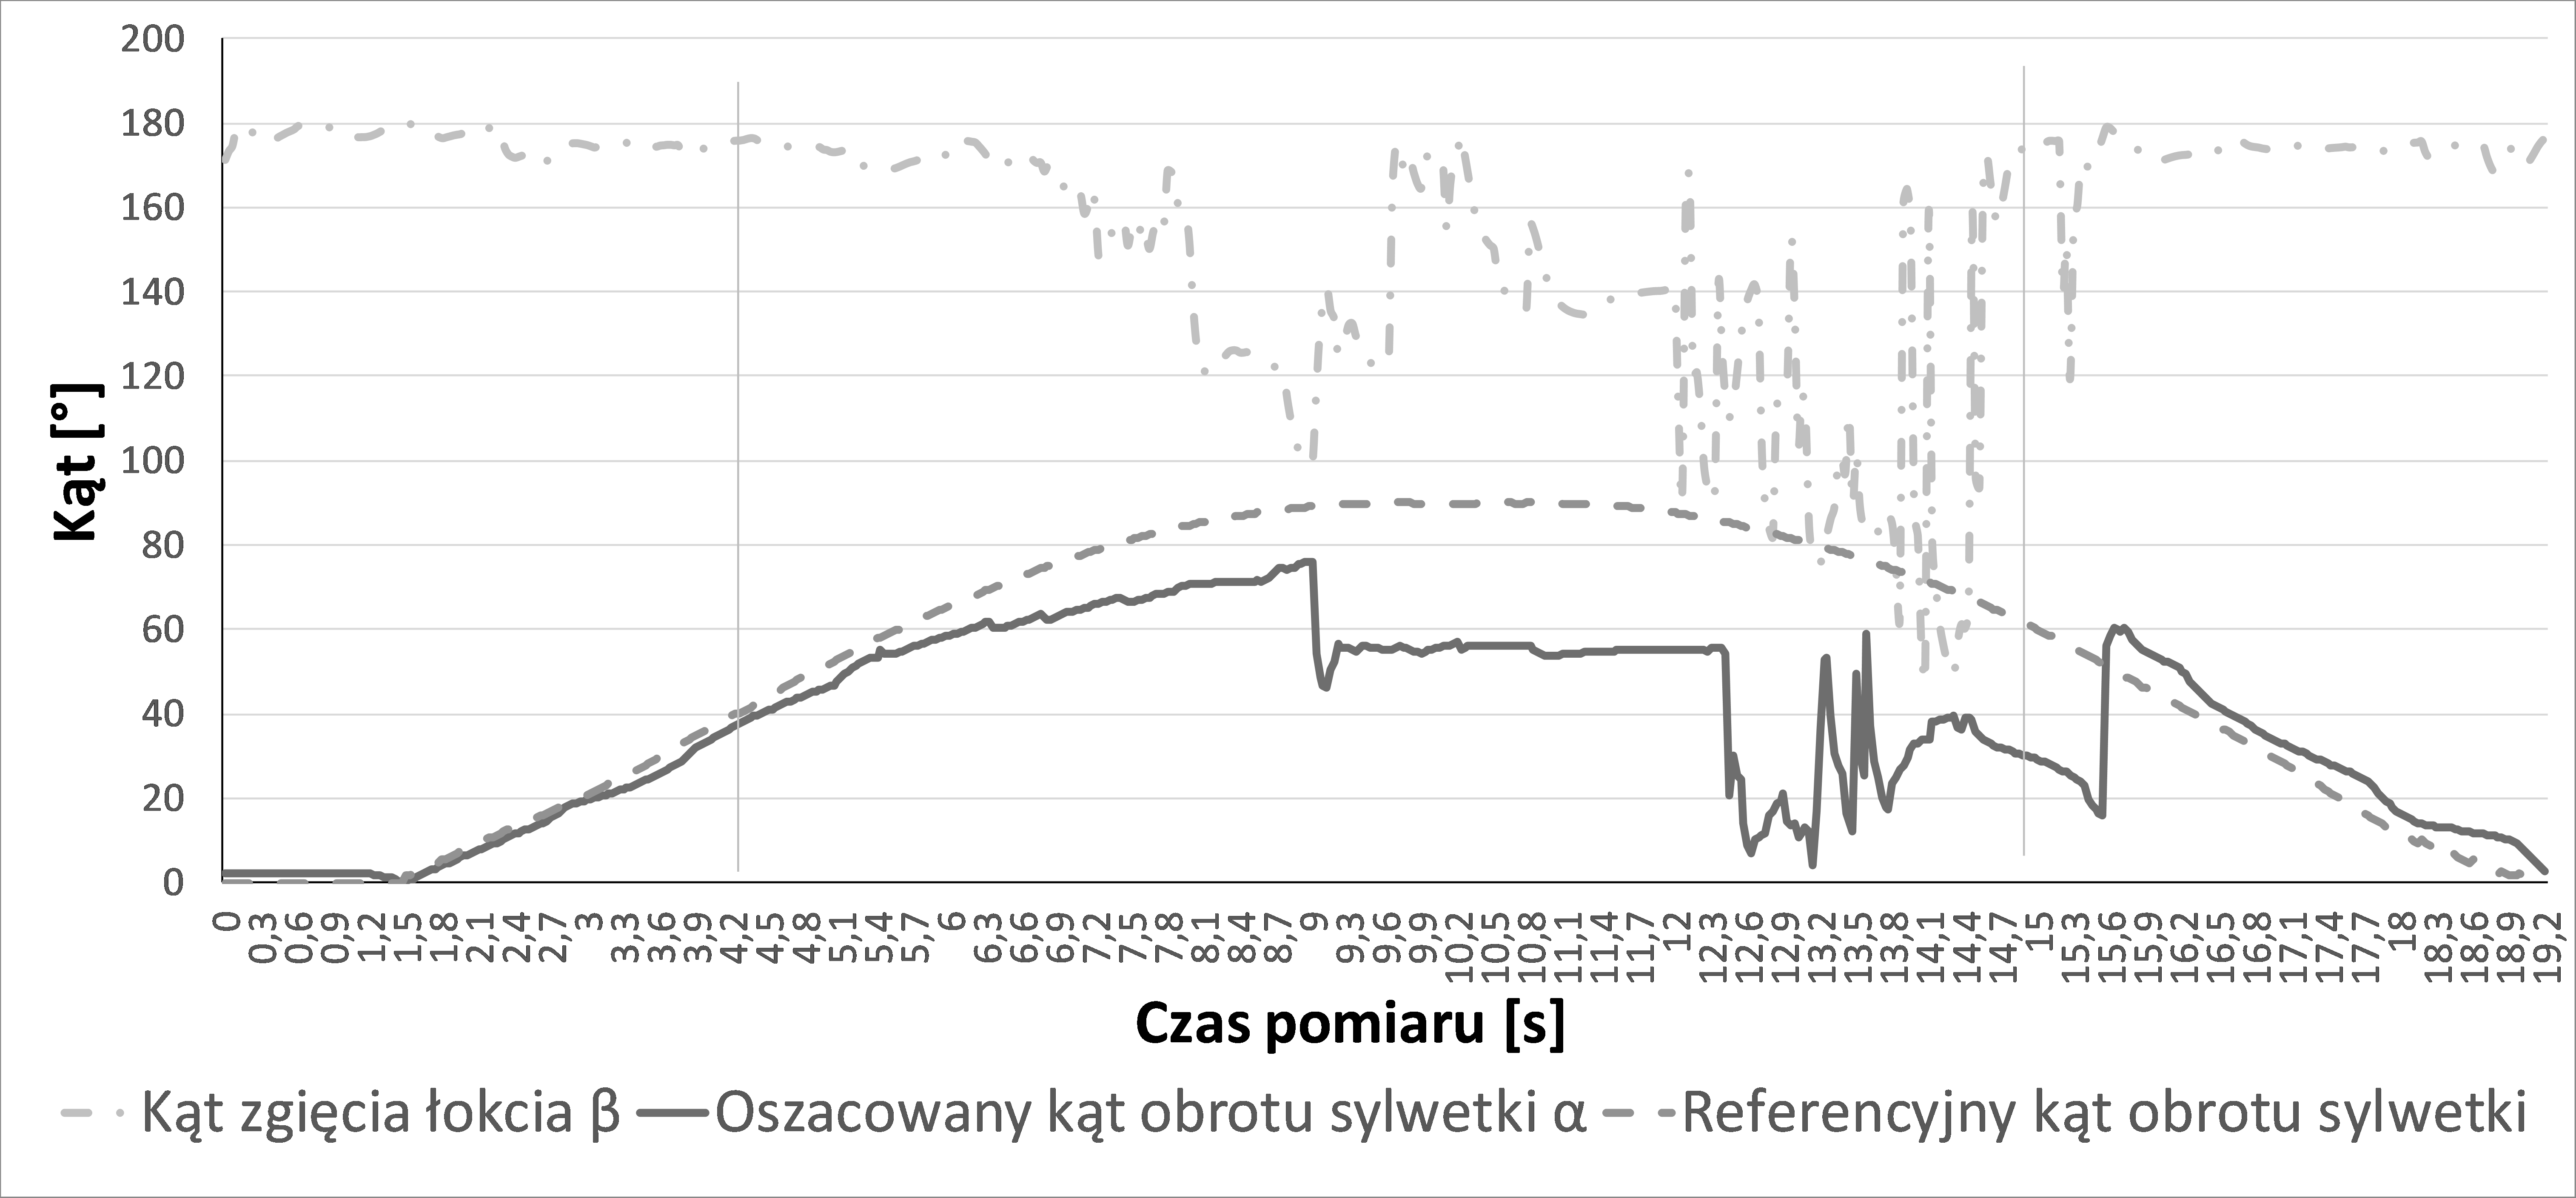
\includegraphics[width=\linewidth]{images/kinectRightHandElbowAngle.png}		
			\caption{Kąt w~łokciu prawej ręki podczas obrotu ciała \emph{(T-pose)} względem kontrolera}
			\label{fig:characteristics:kinect:kinectRightHandElbowAngle}
		\end{subfigure}				
		\caption{Pomiary zależne od kąta obrotu względem Kinecta [źródło własne]}
	\end{figure}
\end{savenotes}
																																					
																																					
\subsubsection*{Szacowanie odległości pomiędzy kontrolerem Kinect, a~śledzoną postacią}\label{sssection:distanceEstimation}
Kolejną istotną cechą kontrolera Kinect jest zmieniająca się dokładność szacowania głębi w~zależności od odległości w~jakiej znajduje się śledzona postać. Specyfikacja urządzenia nie zawiera informacji o~niejednorodności dokładności pomiaru, a~jedynie określa zakres w~jakim działa urządzenie. W~trakcie własnych badań, prowadzonych nad charakterystyką kontrolera Kinect, zaobserwowano zmianę dokładności szacowania głębi wraz z~oddalaniem się użytkownika od urządzenia. Eksperyment, dzięki któremu udało się zaobserwować omawianą zmianę dokładności szacowania odległości, polegał na płynnym oddalaniu się od kontrolera Kinect rejestrując uzyskany dzięki niemu pomiar odległości stawu barkowego oraz równoczesny pomiar tej samej odległości za pomocą systemu śledzenia Vicon. Wykres \ref{fig:characteristics:kinect:distanceAccuracy} przedstawia różnicę pomiędzy pomiarami uzyskanymi za pomocą kontrolera Kinect oraz tymi z~systemu Vicon. Pomiary z~systemu Vicon posłużyły jako dane referencyjne odpowiadające rzeczywistej odległości pomiędzy postacią a~kontrolerem Kinect oraz zostały wykorzystane jako dane na osi rzędnych. Jak widać na wykresie \ref{fig:characteristics:kinect:distanceAccuracy} zmiana dokładności oszacowania odległości, w~jakiej znajduje się śledzona osoba od kontrolera Kinect, nie jest funkcją prostoliniową i~wraz z~oddalaniem się postaci od urządzenia pomiarowego zmienia się od niedoszacowania do przeszacowania wartości. Funkcja reprezentująca przybliżony model dokładności oszacowania odległości przez kontroler Kinect, ma postać wielomianu 3-ego rzędu ($y = a_0 + a_1x + a_2x^2 + a_3x^3$). Wzór \ref{eq:characteristics:kinect:distanceAccuracyPoly} przedstawia równanie pozwalające wyznaczyć współczynniki $a_0 ,a_1, a_2, a_3$ szukanego wielomianu. Macierze $X$ i~$Y$ wykorzystane we wzorze \ref{eq:characteristics:kinect:distanceAccuracyPoly} zawierają odpowiednio argumenty i~wartości dla tych argumentów, na podstawie których możliwe będzie wyznaczenie współczynników wielomianu zawartych w~macierzy $A$. W~przypadku omawianego eksperymentu argumentami są wybrane odległości od Kinecta, w~jakich znajdowała się śledzona postać, natomiast wartościami są różnice pomiędzy oszacowaniem Kinecta, a~odległością uzyskaną dzięki pomiarom systemu Vicon we wspomnianych punktach (argumentach).
																																							
\begin{equation}
	\begin{split}
		X = 	\begin{bmatrix}
		x_1^0&x_1^1&x_1^2&x_1^3\\
		x_2^0&x_2^1&x_2^2&x_2^3\\
		x_3^0&x_3^1&x_3^2&x_3^3\\
		\dots\\
		x_n^0&x_n^1&x_n^2&x_n^3
		\end{bmatrix} ,
		A &= 	\begin{bmatrix}
		a_0\\a_1\\a_2\\a_3
		\end{bmatrix} ,
		Y = 
		\begin{bmatrix}
			y_0 \\y_1\\y_2\\\dots\\y_n
		\end{bmatrix} \\
		& \\
		X^TXA &= X^TY
	\end{split}
	\label{eq:characteristics:kinect:distanceAccuracyPoly}
\end{equation}
gdzie:
\begin{conditions}
	n			& liczba uzyskanych próbek pomiarowych,																\\
	X			& macierz zawierająca argumenty,																\\
	A			& macierz szukanych współczynników funkcji,																\\
	Y			& macierz wartości uzyskanych w~punktach pomiarowych.																\\
\end{conditions}
																																							
																																							
Na podstawie pomiarów uzyskanych w~trakcie eksperymentu opisanego powyżej, macierz współczynników została wyznaczona jak we wzorze \ref{eq:characteristics:kinect:distanceAccuracyCoef}
\begin{equation}
	\label{eq:characteristics:kinect:distanceAccuracyCoef}
	\begin{bmatrix}
		a_0 \\a_1\\a_2\\a_3
	\end{bmatrix} = 
	\begin{bmatrix}
		- 0.25 \\  0.27 \\- 0.11\\0.02		
	\end{bmatrix}	
\end{equation}
																																							
\pgfplotsset{width=12cm,compat=1.8}
																																							
\begin{savenotes}
	\begin{figure}
		\centering
		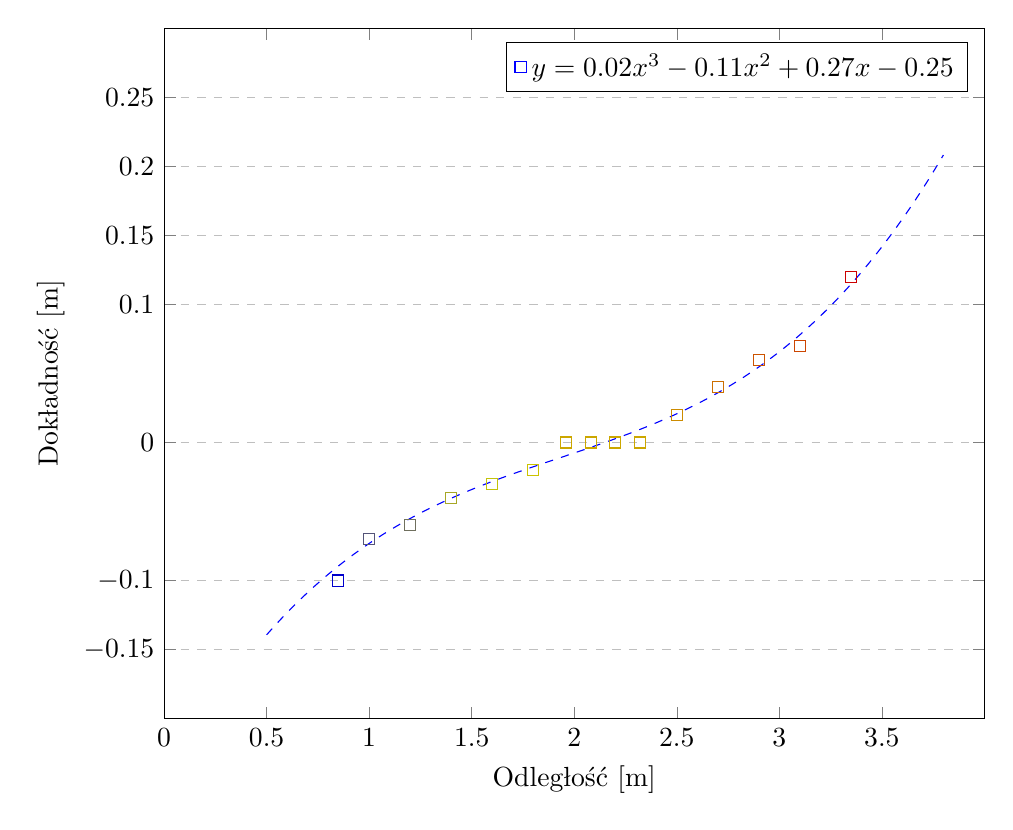
\begin{tikzpicture}
			\begin{axis}[
					xlabel={Odległość [m]},
					ylabel={Dokładność [m]},
					xmin=0, xmax=4,
					ymin=-0.2, ymax=0.3,
					xtick={0,0.5,1,1.5,2,2.5,3,3.5},
					ytick={-0.15,-0.1,-0.5,0,0.5,0.1,0.15,0.2,0.25},
					ymajorgrids=true,
					grid style=dashed,
				]
																																																																																										
				\addplot+[
					only marks,
					scatter,
					color=blue,
					mark=square,
				]
				coordinates {
					(0.85,-0.10)(1.00,-0.07)(1.20,-0.06)(1.40,-0.04)(1.60,-0.03)(1.80,-0.02)(1.96, 0.00)(2.08, 0.00)(2.20, 0.00)(2.32, 0.00)(2.50, 0.02)(2.70, 0.04)(2.90, 0.06)(3.10, 0.07)(3.35, 0.12)
				};
																																																																																										
				\addplot [
					dashed,
					domain=0.5:3.8, 
					samples=100, 
					color=blue,
				]
				{0.0194*x^3 - 0.1125*x^2 + 0.2672*x - 0.2472};
				\legend{$y = 0.02x^3 - 0.11x^2 + 0.27x - 0.25$}
			\end{axis}
		\end{tikzpicture}	
																																																												
		\caption[Przybliżenie dokładności pomiaru głębi względem odległości śledzonej postaci od kontrolera Kinect]{Przybliżenie dokładności pomiaru głębi względem odległości śledzonej postaci od kontrolera Kinect [żródło własne].}
		\label{fig:characteristics:kinect:distanceAccuracy}
	\end{figure}
\end{savenotes}
																																									
Należy zauważyć, że zaprezentowana na wykresie \ref{fig:characteristics:kinect:distanceAccuracy} charakterystyka oszacowania odległości pomiędzy kontrolerem Kinect a~użytkownikiem dotyczy obszaru roboczego tego kontrolera (rys. \ref{fig:characteristics:kinect:range}). W~związku z~tym, dokładność oszacowania pozycji poszczególnych stawów w~modelu szkieletowym użytkownika jest uzależniona od tego, gdzie on się znajduje i~należy to uwzględnić w~prowadzonych obliczeniach, aby wykazane niedokładności skorygować. Jest to o~tyle istotne, że na podstawie uzyskanych wyników, przestrzeń, w~której szacowanie odległości pomiędzy użytkownikiem a~Kinectem jest zbliżone do faktycznej odległości, wynosi jedynie $0.3m$ pomiędzy $2m$, a~$2.3m$ od kamery.  
																																							
																																							
																																									
\subsection{Urządzenia inercyjne}\label{sec:characteristics:imu}
																																									
Urządzenia inercyjne są czujnikami, których działanie opiera się na obserwacji i~mierzeniu wielkości fizycznych, jakie działają na te czujniki w~trakcie ruchu oraz w~spoczynku. Wyróżniamy dwa podstawowe czujniki inercyjne: akcelerometr mierzący przyspieszenia liniowe oraz żyroskop mierzący prędkości kątowe. Choć urządzenia te są znane i~stosowane od dawna, dopiero z~chwilą ich implementacji w~formie mikroukładów elektromechanicznych (MEMS -- \emph{microelectromechanical systems}) stały się one powszechnie dostępne i~stosowane na przukład w~telefonach, czy systemach nawigacji wewnątrz budynków (INS -- \emph{indoor navigation systems}). W~badaniach przedstawionych w~niniejszej pracy, wykorzystany został układ o~symbolu MPU-6050 firmy InvenSense integrujący oba te czujniki (tabela \ref{tab:characteristics:mpu:spec} zawiera podstawowe parametry pracy tego układu). Układ ten oprócz wcześniej wspomnianych czujników posiada wbudowany termometr oraz procesor ruchu pozwalający na przetworzenie danych pomiarowych i~udostępnienie ich w~postaci kwaternionu reprezentującego orientację układu w~przestrzeni. Algorytm wyznaczania orientacji układu, zaimplementowany w~tym procesorze, nie został jednak opublikowany w~żadnej dokumentacji, w~związku z~czym funkcjonalność ta nie była wykorzystywana w~badaniach.
																																									
\begin{table}[h]
	\caption[Zestawienie podstawowych parametrów pracy układu MPU-6050]{Zestawienie podstawowych parametrów pracy układu MPU-6050\footfullcite{footnote:ivenSense:MPU6050}}
	\label{tab:characteristics:mpu:spec}
	\noindent
	\small
	\centering
	\begin{tabular}{|p{5cm}|p{8cm}|}
		\hline 
		Osie pomiaru:                             & X, Y, Z \newline (układ współrzędnych widoczny na rys. \ref{fig:characteristics:imu:space})               \\
		\hline
		Interfejs komunikacyjny:                  & I2C (TWI) - 400 kHz                                                                                           \\
		\hline
		Rozdzielczość danych:                   & 16-bitów dla każdej osi                                                                                     \\
		\hline
		Zakres pomiarowy  \newline akcelerometru: & programowalny: \newline $\pm2g$, \textbf{$\pm4g$}, $\pm8g$, $\pm16g$                                          \\
		\hline
		Zakres pomiarowy żyroskopu:              & programowalny: \newline $\pm250\degree/s$, \textbf{$\pm500\degree/s$}, $\pm1000\degree/s$, $\pm2000\degree/s$ \\
		\hline
	\end{tabular} 	
\end{table} 
																																									
We wszystkich badaniach w~niniejszej pracy, w których wykorzystywane są czujniki inercyjne, są one skonfigurowane do pracy w~zakresie  $\pm4g$ dla akcelerometru oraz $\pm500\degree/s$ dla żyroskopu. Zakresy te zostały wybrane na podstawie specyfikacji komercyjnie dostępnego urządzenia pozwalającego na śledzenie ruchu -- Nintendo WiiRemote.
																																									
\begin{savenotes}
	\begin{figure}[!htb]
		\centering 
		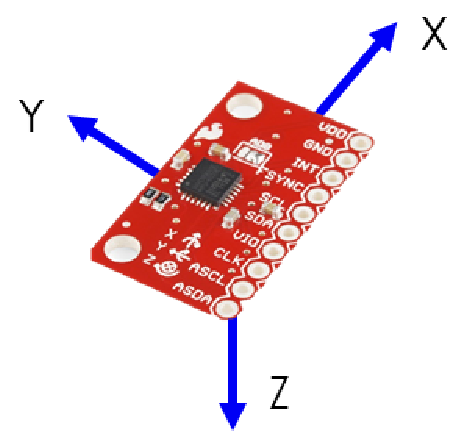
\includegraphics[width=0.35\textwidth]{images/imuCoordinationSpace.eps}	
		\caption{Układ współrzędnych wykorzystywany w~czujnikach MPU--6050}
		\label{fig:characteristics:imu:space}
	\end{figure}
\end{savenotes}
																																											
																																											
\subsubsection*{Akcelerometr}
Akcelerometr mierzy siłę działającą na niego w~dowolnym z~trzech kierunków, wyrażoną w~odniesieniu do siły grawitacji w~jednostkach ''g''. Pozwala to na szacunkowe określenie z~jakim przyspieszeniem wzdłuż każdej osi porusza się dany czujnik ($1g =9.80665^m/_{s^2}$). Ze względu na to, że siła grawitacji działa na wszystkie obiekty nieustannie, akcelerometr leżący horyzontalnie na płaskiej powierzchni i~nie poruszający się, będzie wskazywał wartość $1g$ wzdłuż osi równoległej do wektora grawitacji i~$0g$ w~pozostałych dwóch osiach. Pomijając wpływ szumów na odczyty pomiarów z~akcelerometru, jeśli dla nieporuszajacego się czujnika wartości pomiaru będą inne niż podane powyżej, oznacza to, że czujnik jednak nie leży w~pozycji horyzontalnej. Pomiar wynoszący $0g$ we wszystkich trzech osiach oznacza, że dany obiekt spada swobodnie w~orientacji idealnie poziomej.
																																													
\begin{savenotes}
	\begin{figure}[!htb]
		\captionsetup{singlelinecheck=off}
		\begin{subfigure}[b]{0.45\textwidth}
			\includegraphics[width=\textwidth]{images/memsAccelerometerStructure.png}	
			\caption[Struktura wewnętrzna akcelerometru]{Struktura wewnętrzna \footfullcite{footnote:memsAccStructure2016}}
			\label{fig:characteristics:imu:acc:memsA}
		\end{subfigure}
		\hfill																																																						
		\begin{subfigure}[b]{0.45\textwidth}
			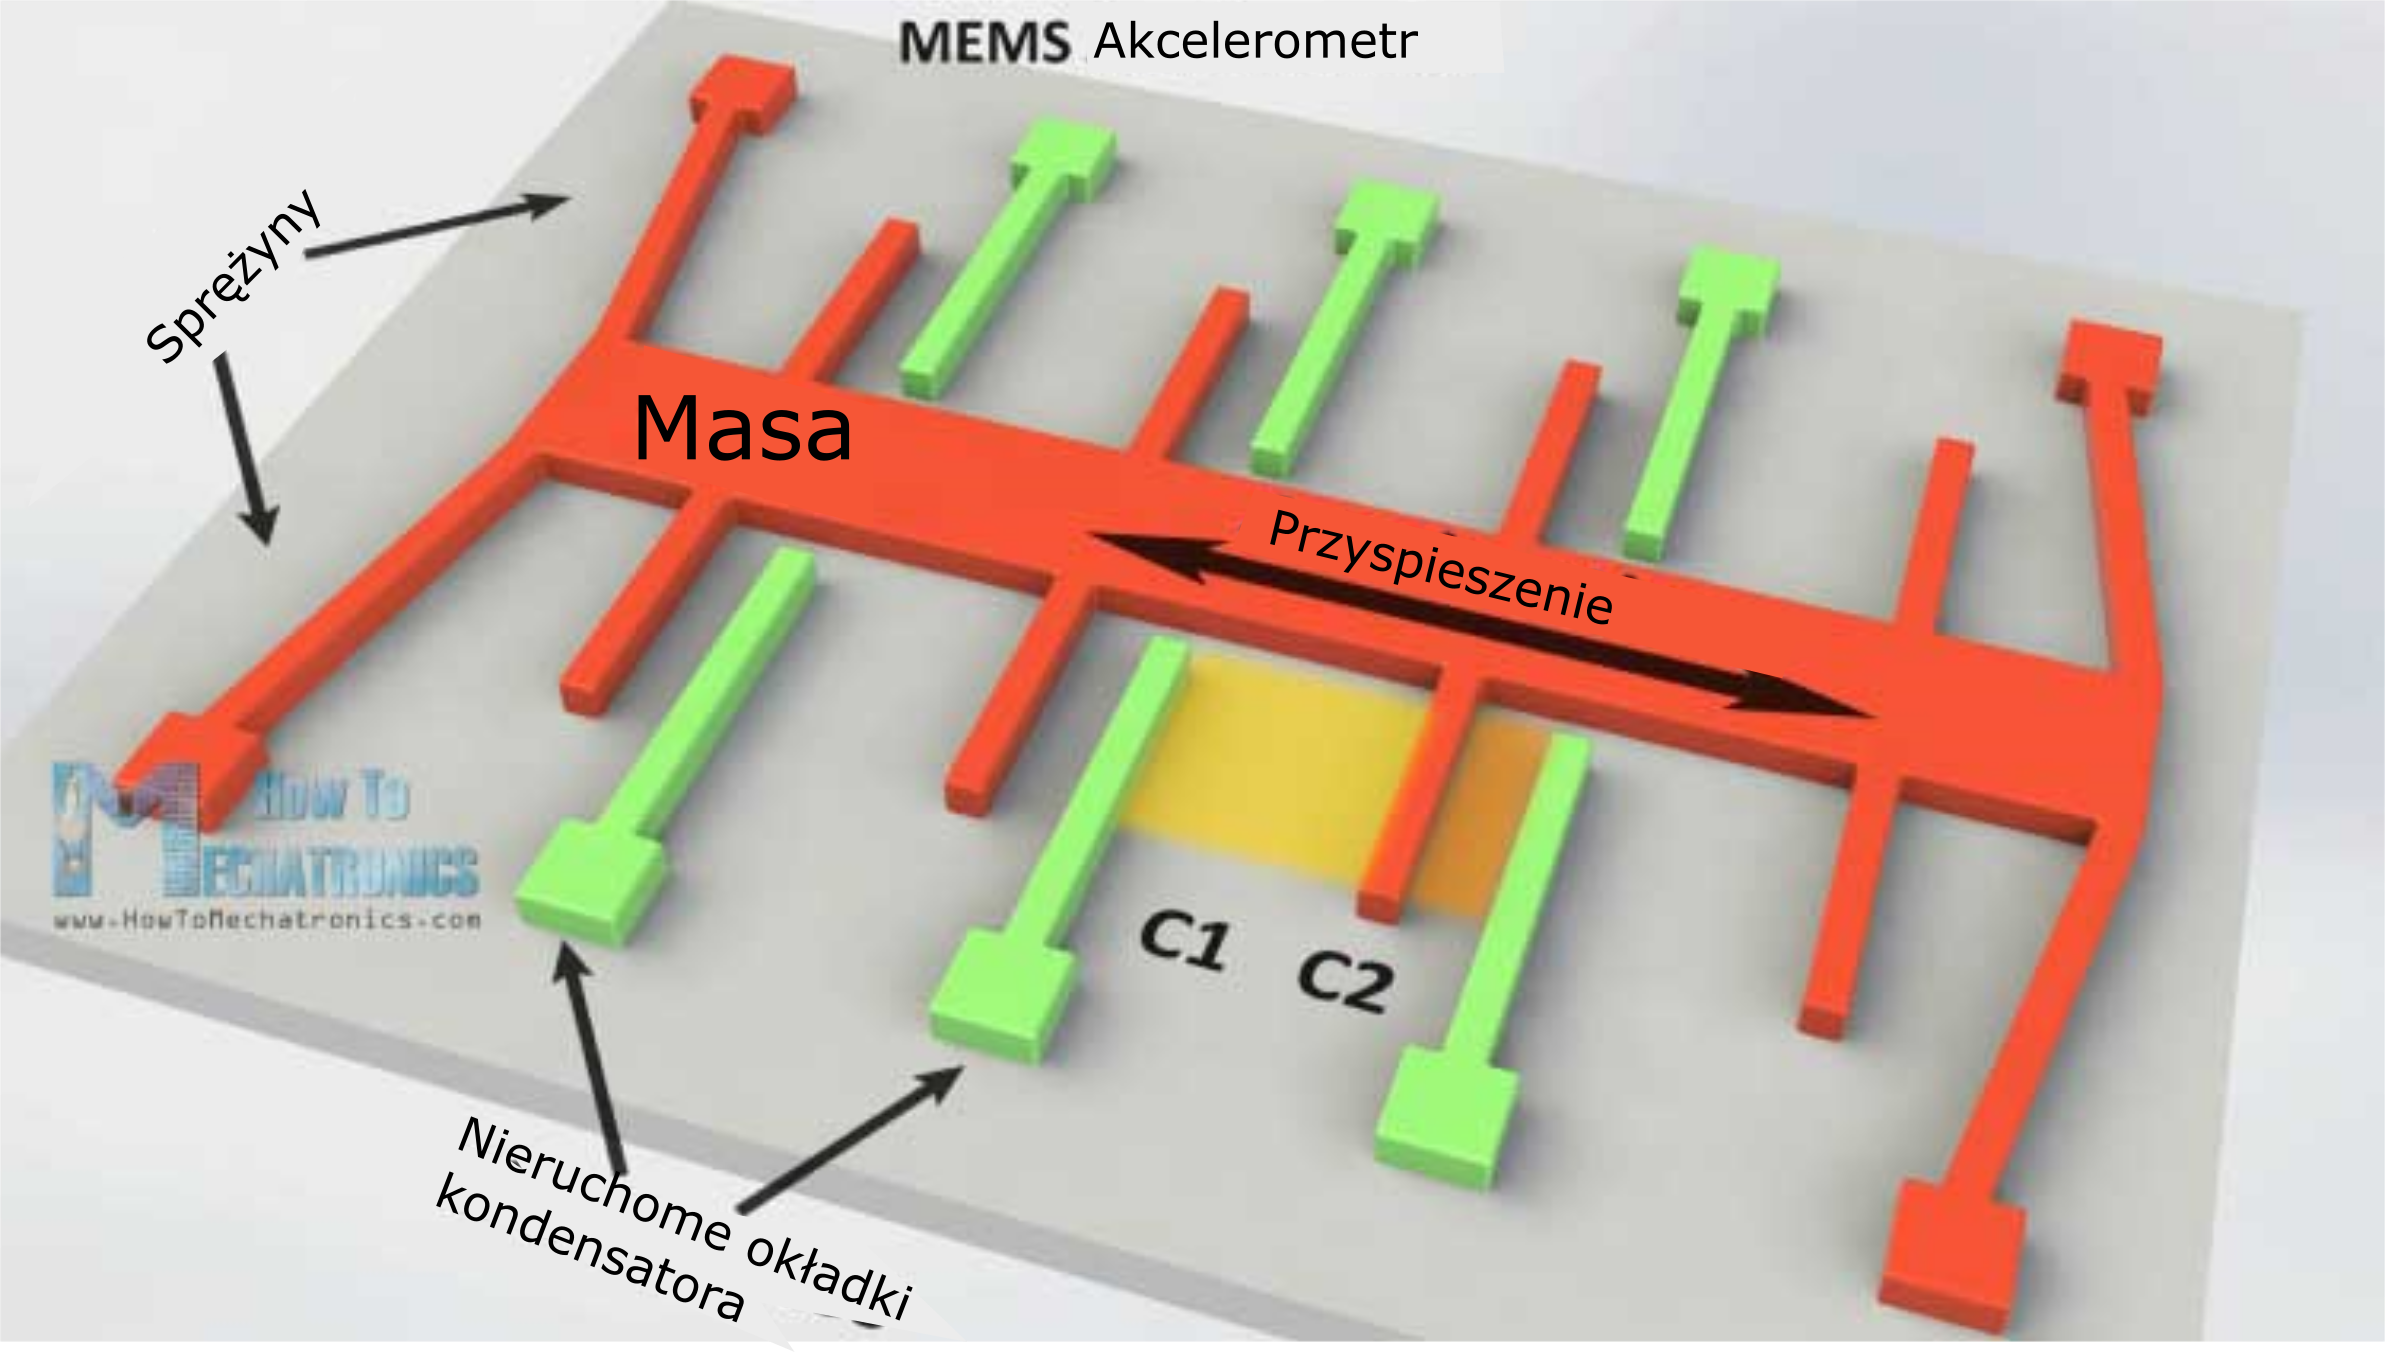
\includegraphics[width=\textwidth]{images/memsAccelerometerIdea.png}		
			\caption[Wizualizacja budowy akcelerometru]{Wizualizacja budowy \footfullcite{footnote:memsAccIdea2016}}
			\label{fig:characteristics:imu:acc:memsB}
		\end{subfigure}				
		\caption{Struktura wewnętrzna akcelerometru w~technologii MEMS}
		\label{fig:characteristics:imu:acc:mems}
	\end{figure}
\end{savenotes}
																																											
																																											
Zastosowany w~tym układzie akcelerometr jest czujnikiem typu pojemnościowego. Oznacza to, że jego wewnętrzna struktura opiera się na układzie ruchomych półprzewodnikowych belek ułożonych pomiędzy analogicznymi, nieruchomymi belkami, które tym samym tworzą układ kondensatorów (rys. \ref{fig:characteristics:imu:acc:mems}). Pomiędzy dwiema sąsiednimi nieruchomymi belkami znajduje się dokładnie jedna belka ruchoma tworząc w~ten sposób parę dwóch kondensatorów o~zmiennych pojemnościach $C_1$ i~$C_2$. Siła działająca na czujnik powoduje przesunięcie się ruchomej belki w~kierunku przyłożonej siły o~dystans $d$. Przyjmując dystans pomiędzy nieruchomymi belkami a~belką ruchomą w~czasie spoczynku jako $d_0$, to przy powierzchni belek, oznaczonej jako $s$, i~stałej dielektrycznej materiału, z~którego wykonane są belki $\epsilon$, pojemności $C_1$ i~$C_2$ określone są wzorem \ref{eq:characteristics:imu:acc:capacitor}.
																																												
\begin{subequations}
	\begin{align}
		C_1 = \frac{\epsilon s}{d_0 + d}             \\ 
		C_2 = \frac{\epsilon s}{d_0 - d}             
		\label{eq:characteristics:imu:acc:capacitor} 
	\end{align}
\end{subequations}
																																												
Następnie, na podstawie wartości $C_1$ i~$C_2$ oraz wartości napięcia elektrycznego jaki zasila układ akcelerometru, możliwe jest wynaczenie wartości napięcia wypływającego z~takiej pary kondensatorów $V_C$ przy podanym napięciu wejściowym $V_0$ za pomocą wzoru \ref{eq:characteristics:imu:capacityToVoltage}.
																																											
\begin{equation}
	V_C = V_0 \frac{C_2-C_1}{C_2+C_1} = V_0\frac{d}{d_0}
	\label{eq:characteristics:imu:capacityToVoltage}
\end{equation}
																																												
Ponieważ wartość napięcia $V_C$ jest zależna od wartości przemieszczenia $d$ ruchomej belki w~układzie dwóch kondesatorów, wartość ta odzwierciedla siłę jaka działa na dany czujnik. Bezpośredni odczyt wartości $V_C$ musi być jednak poddany dodatkowemu przetwarzaniu w~celu określenia kierunku w~jakim zadziałała siła. Kierunek działania siły na czujnik, odzwierciedlony jest w~postaci znaku $+$ albo $-$ przy wartości $V_C$. Następnie możliwe jest wyznaczenie wartości przyspieszenia $a$ działającego na dany czujnik. W~tym celu należy wykorzystać fakt, że siła sprężystości $F_s$ dla małych odkształceń, na podstawie prawa Hooke\'a, jest wprost proporcjonalna do odkształcenia sprężyny (w tym wypadku do przemieszczenia ruchomej belki $d$). Oznaczając przez $f_s$ współczynnik sprężystości charakterystyczny dla materiału, z~którego zbudowana jest dana sprężyna, siłę sprężystości można zdefiniować wzorem \ref{eq:characteristics:imu:springForce}
																																											
\begin{equation}
	F_s = f_s d
	\label{eq:characteristics:imu:springForce}
\end{equation}	
																																												
Wykorzystując drugie prawo Newtona możemy przedstawić związek pomiędzy siłą (Fs) działającą na ciało, jego masą $m$ oraz jego przyspieszeniem $a$. Na tej podstawie wzór \ref{eq:characteristics:imu:springForce} można przekształcić do postaci określonej wzorem \ref{eq:characteristics:imu:springForceNewton}.
																																											
\begin{equation}
	F_s = ma = f_s d
	\label{eq:characteristics:imu:springForceNewton}
\end{equation}	
																																											
Następnie łącząc ze sobą wzory \ref{eq:characteristics:imu:capacityToVoltage} oraz \ref{eq:characteristics:imu:springForceNewton} możemy wyznaczyć wartość przyspieszenia jak we wzorze \ref{eq:characteristics:imu:acceleration}.
																																											
\begin{equation}
	ma = f_s d \Rightarrow a~= \frac{f_s}{m} d = \frac{f_s}{m} \frac{d_0 V_C}{V_0}
	\label{eq:characteristics:imu:acceleration}
\end{equation}
																																											
Szczegółowy opis budowy i~działania akcelerometrów zbudowanych w~architekturze MEMS można znaleźć w~pracy Mateja Andrejasica z~Uniwersytetu w~Lubljanie \cite{Andrejasic2008}.
																																											
\subsubsection*{Żyroskop}
Budowa wykorzystanego żyroskopu, podobnie jak akcelerometru, opiera się na układzie kondensatorów o~zmiennej pojemności, jednak w~tym przypadku są one dodatkowo wprawione w~drgania. Działanie takiego żyroskopu opiera się na efekcie Coriolisa \footfullcite{footnote:memsAccIdea2016}. Budowę i~uproszczony sposób działania czujnika przedstawia rysunek \ref{fig:characteristics:imu:gyro:mems}. Wykorzystane urządzenie mierzy prędkość kątową wokół 3 osi, wyrażoną w~stopniach na sekundę ($^\degree/_s$), odpowiadającą konwencji nazewniczej związanej z~reprezentacją obrotów w~postaci kątów Eulera (rozdział \ref{chap:orientstionRep}). 
																																													
\begin{savenotes}
	\begin{figure}[!htb]
		\captionsetup{singlelinecheck=off}		
		\begin{subfigure}[b]{0.45\textwidth}
			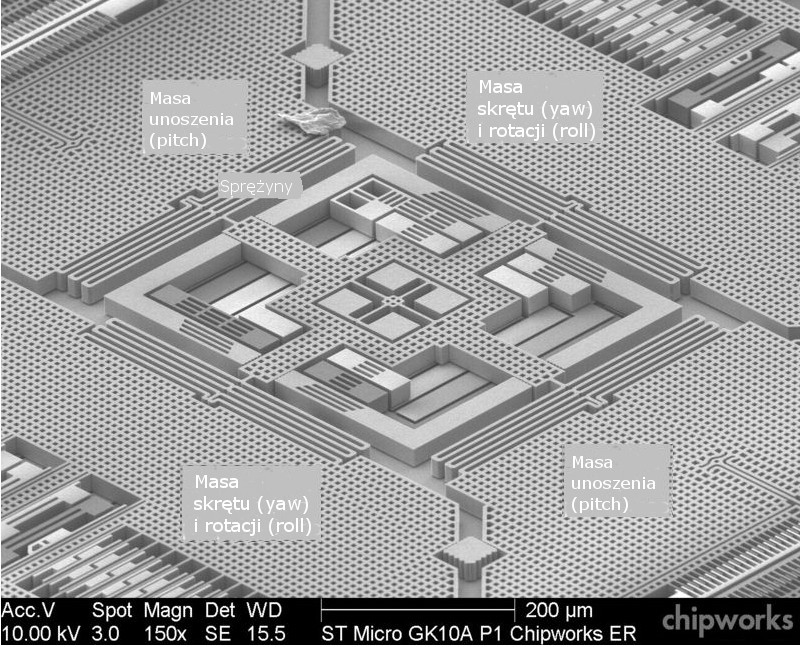
\includegraphics[width=\textwidth]{images/memsGyroscopeStructure.jpg}	
			\caption[Struktura wewnętrzna żyroskopu]{Struktura wewnętrzna \footfullcite{footnote:memsGyroStructure2016}}
			\label{fig:characteristics:imu:gyro:memsA}
		\end{subfigure}
		\hfill																																																									
		\begin{subfigure}[b]{0.45\textwidth}
			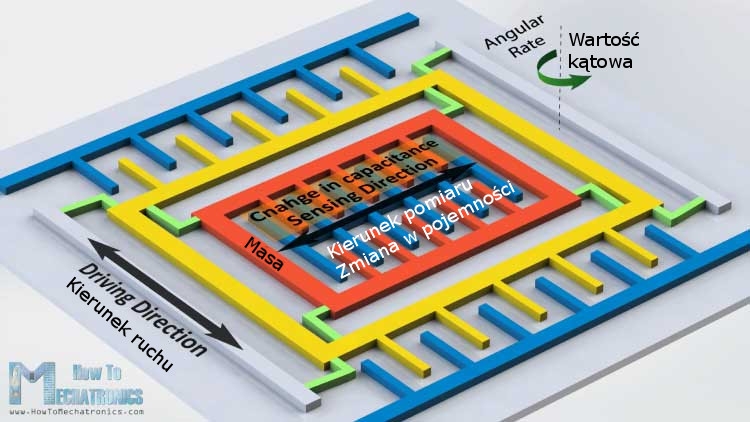
\includegraphics[width=\textwidth]{images/memsGyroscopeIdea.jpg}		
			\caption[Wizualizacja budowy żyroskopu]{Wizualizacja budowy \footfullcite{footnote:memsAccIdea2016}}
			\label{fig:characteristics:imu:gyro:memsB}
		\end{subfigure}				
		\caption{Struktura wewnętrzna żyroskopu w~technologii MEMS}
		\label{fig:characteristics:imu:gyro:mems}
	\end{figure}
\end{savenotes}
																																															
\subsection{Ograniczenia w~działaniu czujników inercyjnych}
Ograniczenia w~działaniu obu czujników inercyjnych można rozdzielić na te dotyczące ogólnie urządzeń stworzonych w~architekturze MEMS, a~tym samym wynikające z~ich budowy i~właściwości fizycznych, oraz na te charakterystyczne dla poszczególnych rodzajów czujników związane z~ich działaniem np.: szum danych, czy wpływ temperatury urządzenia na uzyskiwane pomiary.

Pomiary dostarczane przez oba czujniki zawierają szum, który w~znaczący sposób wpływa na dalsze obliczenia. Do określenia charakteru zakłóceń pomiaru najczęściej wykorzystuje się wariancje oraz odchylenie Allana\cite{Allan1966}, która to metoda została przyjęta przez IEEE jako standardowa do określania szumu w~IMU \cite{IeeeAccSpec}. Z uzyskanych za pomocą tej metody wyników można odczytać, że dwoma typami szumów, które przeważają w~sygnalne uzyskanym z~żyroskopu i~akcelerometru są: błądzenie losowe związane z~mierzonymi wielkościami (ang. \emph{angular/velocity random walk}), a~także szum o~wysokiej częstotliwości oraz niestabilność błędu systematycznego (ang. \emph{bias instablity}) o~niskiej częstotliwości. Fakt występowania obu szumów w~czujnikach inercyjnych jest dodatkowo powiązany z~różnymi charakterystykami częstotliwościowymi właściwych sygnałów. Dla akcelerometru, mierzącego działające na niego siły w~odniesieniu do siły grawitacji, sygnał prawidłowy jest o~niskiej częstotliwości, więc szczególnego znaczenia nabiera zakłócenie i~zmienność wartości błędu systematycznego. Z kolei sygnał zarejestrowany przez żyroskop jest wysokoczęstotliwościowy, więc błądzenie losowe wpływa na uzyskane wyniki.

Jednym z~czynników wpływających na jakość pomiarów uzyskiwanych za pomocą czujników tworzonych w~architekturze MEMS jest temperatura pracy tych urządzeń. Jej wpływ na uzyskiwane wyniki, jak w~swojej analizie wskazują Liu i in. \cite{Liu2007, Liu2015}, mają 3 czynniki: moduł Younga, deformacja materiału pod wpływem temperatury oraz naprężenia materiału. Każdy z~tych czynników wpływa na możliwości przepływu prądu w~omawianych układach, co bezpośrednio wpływa na jakość interpretacji zgromadzonych ładunków w~kondensatorach układów MEMS. Zgodnie ze specyfikacją układu MPU-6050, temperatura neutralna dla ich pracy to 25 $\degree C$, a~błąd związany z~temperaturą urządzenia zmienia się nieliniowo. Zmiana temperatury układów MEMS wynika z~temperatury otoczenia, w~której pracują oraz z~naturalnego wydzielania się ciepła podczas pracy. W~wyniku własnych eksperymentów udało się zaobserwować wpływ zmiany temperatury na uzyskane pomiary przyspieszenia ziemskiego w~zakresie temperatur 10-50 $\degree C$ (rys. \ref{fig:characteristics:imu:temp}). Ponieważ temperatura pracy urządzeń umieszczonych przy ciele stabilizuje się w okolicach 32 $\degree C$, czynnik ten musi być wzięty pod uwagę i~skorygowany przed obliczeniami bazującymi na danych akcelerometru. Podobnej zależności nie zaobserwowano w~przypadku używanych żyroskopów. Prawdopodobną przyczyną jest fakt, że temperatura wpływa na sygnały o~niskiej częstotliwości, które są odfiltrowane w~trakcie odczytu pomiarów. Wynika to z~faktu, że prawidłowy sygnał, jaki rejestrowany jest przez żyroskop, powinien mieć wysoką częstotliwość, a~w~związku z~tym cały sygnał przetwarzany jest filtrem górnoprzepustowym. W~takim przypadku szum niskiej częstotliwości jest w~dużym stopniu usunięty z~uzyskiwanych pomiarów.
																																															
\begin{savenotes}
	\begin{figure}
		\centering
		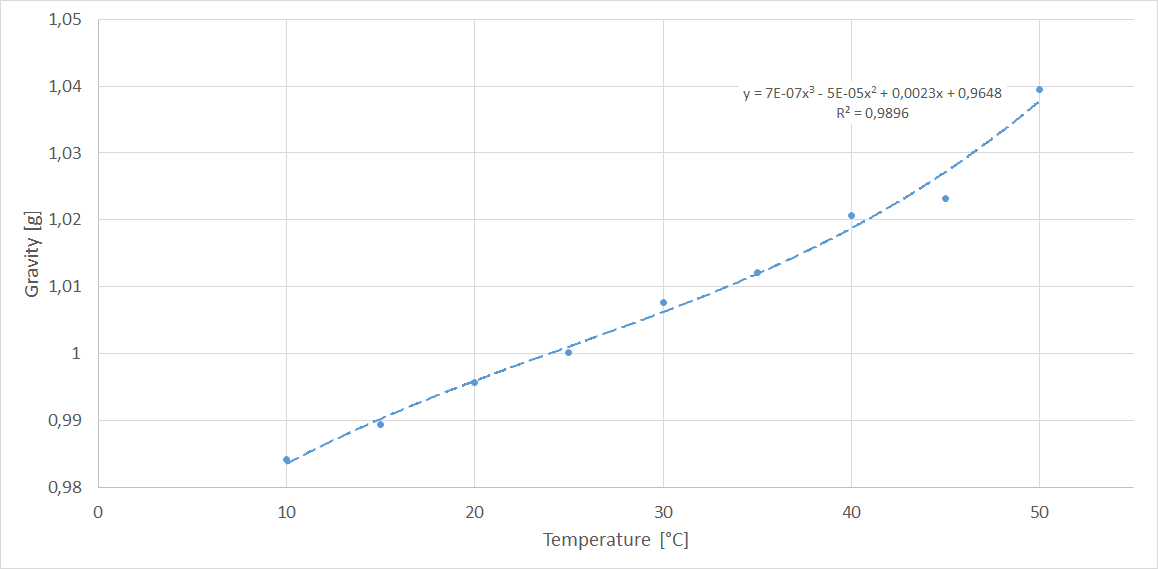
\includegraphics[width=0.8\textwidth]{images/temp.png}
		\caption[Pomiar przyspieszenia ziemskiego w~przedziale temperatur 10-50$\degree C$]{Pomiar przyspieszenia ziemskiego w~przedziale temperatur 10-50$\degree C$ [źródło własne]}
		\label{fig:characteristics:imu:temp}
	\end{figure}
\end{savenotes}
																																																	
Do precyzyjnego określenia orientacji, w~przestrzeni urządzenia pomiarowego złożonego z~czujników inercyjnych i~magnetycznych, nie powinno się bazować jedynie na pojedynczym czujniku (przykładowo, wyłącznie na żyroskopie), ale należy połączyć ze sobą sygnały (ang. \emph{data fusion}) z~kilku różnych czujników na przykład: akcelerometru i~żyroskopu, czy żyroskopu i~magnetometru. Wynika to z~szumów jakie występują w~mierzonych sygnałach i~konieczności ich odfiltrowania. Ponieważ charakterystyki szumów i~sygnałów mierzonych przez każdy z~czujników różnią się od siebie, to właśnie zsynchronizowane łączenie danych daje rezultaty lepsze niż na przykład zastosowanie filtracji na pojedynczym sygnale. Jakość uzyskanych wyników takiego łączenia danych jest zależna od wybranej metody (rozdział \ref{chap:appx:filters}) oraz posiadanej wiedzy dotyczącej charakterystyk urządzeń. W~przypadku zastosowania pary akcelerometr -- żyroskop, pomimo tego, że każdy z~nich jest urządzeniem 3-osiowym, możliwe jest wyznaczenie orientacji jedynie względem 2 osi. Ograniczenie to wynika z~pomiarów, jakie można uzyskać z~akcelerometru. Aby móc połączyć ze sobą dane z~obu czujników, zarówno akcelerometr jak i~żyroskop muszą udostępnić dane dotyczące obrotów wokół tych samych osi. O ile żyroskop faktycznie dokonuje pomiaru prędkości kątowych wokół wszystkich 3 osi, o~tyle akcelerometr podaje informację o~tym jak czujnik jest obrócony tylko względem dwóch osi. Dla akcelerometru, obrót wokół osi działania siły grawitacji (obrót względem osi $Z$ na rys. \ref{fig:characteristics:imu:space}) jest niemierzalny, ponieważ obrót taki nie zmienia wartości z~jaką ta siła działa na czujnik w~danej chwili. Z tego zaś powodu, orientacja względem osi działania siły grawitacji nie jest wyznaczona drogą łączenia danych z~akcelerometru i~żyroskopu, a~jedynie może być wyznaczona na podstawie całkowania prędkości kątowej zmierzonej przez sam żyroskop, co jest obarczone znaczącymi błędami z~uwagi na zaszumienie danych. W~związku z~tym nie bierze się tej wartości pod uwagę w~obliczeniach i~przyjmuje się, że urządzenia oparte tylko na parze czujników inercyjnych określają orientację względem dwóch osi.

Opisane w~niniejszym rozdziale urządzenia pomiarowe: kontroler Microsoft Kinect oraz czujniki inercyjne: akcelerometr i~żyroskop, są wykorzystywane do budowy dwóch różnych systemów śledzenia ruchu. Wykorzystując kontroler Microsoft Kinect można zbudować optyczny system śledzenia ruchu nie wykorzysujący markerów (roz. \ref{chap:mocaps:Kinect}), a~z kolei akcelerometry i~żyroskopy stanowią podstawę dla nieoptycznych inercyjnych systemów śledzenia ruchu (roz. \ref{chap:mocaps:IMU}). Opierając się na charakterystykach zarówno wspomnianych urządzeń pomiarowych jak i~cechach systemów śledzania ruchu na nich opartych, badacze zwrócili uwagę na możliwość tworzenia hybrydowych systemów śledzenia ruchu, które opierają się na kontrolerze Kinect, akcelerometrach oraz żyroskopach. Tworzenie takich hybrydowych systemów śledzenia ruchu możliwe jest dzięki temu, że urządzenia pomiarowe, które wykorzystują, mogą się wzajemnie uzupełniać w~działaniu.
																																																			
\section{Systemy hybrydowe łączące optyczny system śledzenia ruchu bez markerów oraz inercyjny system śledzenia ruchu} \label{sec:literature:hybrids}
Poszukiwanie rozwiązań pozwalających na łączenie ze soba optycznych systemów śledzenia ruchu bez markerów oraz inercyjnych systemów śledzenia jest zagadnieniem stosunkowo często spotykanym w~literaturze. Wiele ośrodków badawczych na całym świecie prowadzi badania w~tym obszarze mające na celu zwiększenie dokładności pozycjonowania stawów i~śledzenia ich ruchu. Obecnie, dzięki powszechnej dostępności urządzeń pomiarowych takich jak kontroler Kinect oraz akcelerometry i~żyroskopy, jak również dzięki badaniom związanym z~ich połączeniem w~jeden system, można budować hybrydowe systemy śledzenia ruchu o~wysokiej dokładności, które mogą być dostępne do użytku domowego. Otwiera to z~kolei wiele możliwości w~obszarze zastosowań takich systemów, jak chociażby zaawansowane systemy do telerehabilitacji, czy programy do precyzyjnych treningów sportowych. W~dalszej części pracy przedstawione zostaną te opracowania, które wykorzystują kamery RGB-D dostępne na rynku konsumenckim (w~szczególności kontroler Kinect) oraz urządzenia inercyjne lub magnetyczne. 

W 2014 roku Destelle i in. \cite{Destelle2014} zaproponował połączenie ze sobą kontrolera Kinect oraz systemu inercyjnego, w~celu stworzenia kompletnego systemu śledząco--pozycjonującego, nie korzystającego z~sygnału GPS oraz zaawansowanych systemów LPM w~celu określenia położenia użytkownika na scenie. W~rozwiązaniu autorów Kinect został wykorzystany na dwa sposoby:
\begin{enumerate}
	\item Jako system definiujący model szkieletowy.
	\item Jako system odpowiedzialny za śledzenie położenia aktora na scenie.
\end{enumerate}
																																																	
W omawianym rozwiązaniu autorzy zdecydowali się na wykorzystanie urządzeń inercyjnych stworzonych przez firmę X-IO Technologies \footfullcite{footnote:xIo}. Urządzenia inercyjne firmy X-IO Technologies to układy zbudowane na bazie czujników inercyjnych oraz czujników inercyjnych wspieranych przez czujnik magnetyczny. Łączenie danych z~tych czujników, mające na celu określenie orientacji przestrzennej urządzenia, stosuje autorską metodę założyciela tej firmy, nazwaną jego nazwiskiem -- metodę Madgwicka.

Aby uniknąć konieczności budowania modelu szkieletowego na podstawie własnych pomiarów, na potrzeby systemu inercyjnego, autorzy postanowili wykorzystać estymację szkieletu dokonywaną przez Kinecta. Aby uniknąć problemów związanych ze zmiennością szacowania długości poszczególnych kości, a~co za tym idzie zmiennością proporcji modelu szkieletowego, niezbędne pomiary pozwalające wyznaczyć model szkieletowy dokonywane są tylko raz w~czasie inicjalizacji systemu i~zostają przyjęte jako stałe na cały czas trwania śledzenia ruchu. W~trakcie śledzenia ruchu rolą urządzeń inercyjnych było określenie orientacji przestrzennej tych kości, do których takie moduły były przymocowane, a~rolą Kinecta było określenie położenia całego modelu postaci na scenie. Pozycjonowanie modelu na scenie zostało zrealizowane poprzez śledzenie przez kontroler Kinect położenia pojedynczego punktu znajdującego się na korpusie obserwowanej postaci. Przemieszczenie tego pojedynczego punktu traktowane jest jako przemieszczenie całego wyznaczonego modelu szkieletowego. W~omawianym artykule, Destelle wskazuje średniokwadratowy błąd wyznaczania kątów zgięcia kończyn w~stawach na $4\degree$ -- $14\degree$ w~zależności od stawu, wobec błędu średniokwadratowego w~przedziale $10\degree$ -- $30\degree$ dla tych samych stawów w~przypadku pomiaru kątów wyłącznie za pomocą samego kontrolera Kinect. Warto jednak zauważyć, że w~przypadku pomiarów obarczonych największym błędem średniokwadratowym następowała czasowa utrata śledzenia poszczególnych stawów. Autor nie zamieścił natomiast żadnych danych pozwalających na oszacowanie dokładności wyznaczenia pozycji poszczególnych stawów. Łatwo można zauważyć, że system zaproponowany przez Destelle nie wykorzystuje w~pełni możliwości łączenia danych z~obu urządzeń, gdyż wykorzystywane są one w~odrębnych obszarach i~mają minimalny wpływ na siebie. Stąd, porównanie dokładności samego Kinecta z~dokładnością systemu hybrydowego w~zakresie mierzenia zgięcia kończyn w~stawach jest de facto porównaniem dokładności tego pierwszego z~urządzeniem Madgwicka. Z drugiej zaś strony, omawiany system dobrze pokazuje zasadność wykorzystania w~badaniach łatwo dostępnych i~tanich urządzeń inercyjnych, które pozwalają poprawić wyniki kontrolera Kinect.																																																	
Bo i in. \cite{Bo2011a} w~swoich badaniach w~2011 roku zaproponowali metodę szacowania kąta stawu kolanowego wykorzystując układ czujników inercyjnych o~pięciu stopniach swobody (2 stopnie swobody dla żyroskopu i~3 stopnie swobody dla akcelerometru) oraz Kinecta. Metoda ma niejako 2 tryby działania: dla sytuacji kiedy dane z~Kinecta są dostępne i~wtedy kiedy ich brakuje. W~obu przypadkach to czujniki inercyjne są wykorzystywane do oszacowania kąta zgięcia kończyny w~obserwowanym stawie, przy czym wartości te obliczane są osobno dla żyroskopu ($\Theta_G$) i~akcelerometru ($\Theta_A$). Oszacowanie wartości kąta, wykorzystuje całkowanie pomiarów żyroskopu ($\tilde{\omega}_y$) zgodnie ze wzorem \ref{eq:literature:bo:gyro} oraz bazuje na obliczeniach trygonometrycznych uwzględniających stosunek siły działającej na akcelerometr w~wybranych osiach ($f_x , f_z$) do siły grawitacji $g$ według wzoru \ref{eq:literature:bo:acc}. Następnie wartości te są ze sobą łączone z~wykorzystaniem liniowego filtru Kalmana.
																																																	
\begin{equation}
	\Theta_G = \int{\tilde{\omega}_y dt}
	\label{eq:literature:bo:gyro}
\end{equation}
																																																	
\begin{equation}
	\Theta_A = \alpha \arccos{\frac{f_x}{\norm{g}}} + (1 - \alpha) \arcsin{\frac{f_z}{\norm{g}}}
	\label{eq:literature:bo:acc}
\end{equation}
																																																	
W przypadku dostępności danych z~Kinecta, dodatkowym krokiem jest korekta pomiarów na podstawie danych z~tego urządzenia. Obliczana jest wówczas różnica pomiędzy wartościami wyznaczonymi z~czujników inercyjnych i~z Kinecta, a~wartość różnicy uwzględniana jest jako korekta estymacji kąta dokonanej jedynie na podstawie pomiarów akcelerometru.
																																																	
Metoda zaproponowana przez Bo i in. opiera się na założeniu, że Kinect jest wystarczająco dokładnym urządzeniem, aby jego pomiary przyjąć jako referencyjne i~na ich podstawie dokonywać korekty innych pomiarów. Dokładna analiza zakresów działania Kinecta (dokładność oszacowania odległości osoby śledzonej od kontrolera) przedstawiona w~rozdziale \ref{chap:characteristics} pokazuje, że takie założenie jest prawdziwe dla ruchów, które odbywają się bez istotnej zmiany odległości pomiędzy kontrolerem Kinect a~postacią. Problemem może być jednak śledzenie ruchu rąk przesuwanych do przodu, ponieważ nawet stojąc w~optymalnej odległości od kontrolera (ok. 2m), ręka w~trakcie ruchu najprawdopodobniej nie będzie znajdowała się obszarze, w~którym Kinect szacuje położenie stawów z~dokładnością zbliżoną do pomiarów rzeczywistych. Dodatkowo, przyglądając się badaniom widać, że metoda była testowana w~taki sposób, że staw kolanowy, którego kąt zgięcia podlegał oszacowaniu, był dobrze widoczny i~znajdował się w~stałej odległości od Kinecta. Osoba, której ruch był śledzony, była obrócona bokiem do kontrolera i~na przemian wstawała i~siadała na krześle. Dzięki temu uniknięto problemów związanych z~okluzją oraz zmianą dokładności śledzenia wynikającej ze zmian odległości postaci od kontrolera Kinect.																																																	
Wyniki zamieszczone w~omawianym artykule \cite{Bo2011a} nie pozwalają na ocenę dokładności proponowanej metody względem wartości rzeczywistych. Pokazują one natomiast relację oszacowań będących wynikiem proponowanej metody do pomiarów Kinecta, które zostały przyjęte przez autorów jako referencyjne. Pokazują również, że dzięki wykorzystaniu łączenia danych z~żroskopu i~akcelerometru udało się uzyskać stabilizację pomiarów kąta za pomocą czujników inercyjnych wobec braku stabilności pomiarów każdego z~czujników z~osobna. Zamieszczone wykresy wyraźnie pokazują negatywny wpływ dryfu na wyniki uzyskane za pomocą żyroskopu, objawiające się stopniowym pogarszaniem jakości pomiarów. Dryf ten jest wyraźny i~na podstawie zamieszczonych wykresów można go ocenić na $2^\degree/_s$. Tendencja ta nie jest widoczna w~przypadku pomiarów akcelerometru, jednak zaobserwować można ciągłe, małe odchylenia od pomiaru referencyjnego. Widać także, że wykorzystanie filtru Kalmana w~liniowej postaci jest w~stanie oba te problemy znacznie ograniczyć.																																																	
W 2015 roku Tian i in. \cite{Tian2015a} zaproponował łączenie danych z~czujników inercyjnych za pomocą bezśladowego filtru Kalmana (UKF - \emph{ang. Unscendent Kalman Filter}). W~prezentowanej metodzie autorzy zdecydowali się na korektę uzyskanych wyników za pomocą z~góry narzuconych ograniczeń geometrycznych, wynikających z~modelu biomechanicznego szkieletu ludzkiego. Początkowo autorzy w~swojej metodzie wyznaczają orientację każdej z~kości, których ruch jest śledzony za pomocą modułów inercyjnych. Orientacje te są wyznaczone bez uwzględniania ich poprawności, to znaczy bez sprawdzenia czy w~ogóle możliwe jest, aby człowiek wykonał taki ruch na jaki wskazują pomiary. Dopiero w~następnym kroku następuje weryfikacja uzyskanych oszacowań ze względu na ograniczenia wynikające z~mechaniki ruchu ciała ludzkiego. Pozwoliło to wyeliminować oszacowania obrotów, które w~sposób oczywisty są niepoprawne oraz ograniczyć wpływ dryfu żyroskopu na ostateczny wynik. Przykładem takiego ograniczenia, dzięki któremu można zweryfikować poprawność oszacowania orientacji kości, jest maksymalny kąt, jaki można uzyskać w~łokciu przy wyprostowanej ręce, wynoszący około $180\degree$. Jeśli zatem oszacowanie, na podstawie danych z~czujników, wskazywałoby przykładowo kąt zbliżony do $220\degree$ to można uznać, że jest to oszacowanie błędne. Po zakończeniu fuzji danych z~czujników inercyjnych przeprowadzano weryfikację dostępności pomiarów z~kontrolera Kinect. Jeśli były one dostępne i~były dostatecznie dobrej jakości, zostały one połączone z~wielkościami uzyskanymi z~IMU za pomocą filtru UKF. Autorzy nie podali wprost kryterium jakości pomiarów Kinecta, ale z~treści artykułu można wywnioskować, że takim kryterium jest wariancja położenia konkretnych stawów. Jeśli dane są niewiarygodne, wartość ta jest bardzo duża w~każdym kolejnym przedziale czasowym. Jeśli dane z~Kinecta nie mogą być użyte do ostatecznego wyznaczenia pozycji, algorytm bazuje tylko na pomiarach z czujników inercyjnych i~odpowiednio aktualizuje położenie stawów na bazie wyznaczonego oszacowania. Porównanie uzyskanych wyników z~wynikami referencyjnymi uzyskanymi z~systemu wizyjnego z~markerami, pozwoliło autorom oszacować dokładność ich metody śledzenia poniżej $20\degree$ dla kąta zgięcia łokcia.																																																	
Cechą wspólną powyższych metod jest to, że podstawą ich działania były pomiary z~czujników inercyjnych, a~Kinect stanowił uzupełnienie lub korektę uzyskanych pomiarów. W~przypadku Bo i in. oraz Destelle i in. dane z~Kinecta nie były w~żaden sposób poddane weryfikacji co do ich wiarygodności. Podejście takie było obarczone dużym ryzykiem wprowadzenia dodatkowych błędów do uzyskanego wyniku, które mogło całkowicie wypaczyć wyniki. Metoda zaprezentowana przez Tian i in. wprowadziła krok weryfikujący poprawność danych Kinecta i~wraz z~ograniczeniami wynikającymi z~biomechaniki minimalizowała wpływ zaszumienia danych na ostateczny rezultat. Nie wiadomo jednak jak długo dyskutowana metoda jest w~stanie, w~poprawny sposób, działać bez pomiarów Kinecta. Taki eksperyment nie został opisany w~artykule.																																																	
Kolejną grupę hybrydowych metod łączących sygnały inercyjne z~sygnałami kontrolera Kinect stanowią metody, które wykorzystują w~sposób ciągły oba te źródła. Wymagają one ciągłego analizowania obu sygnałów i~na podstawie ich jakości decydują z~jakim stopniem istotności je połączyć. W~2014 roku Feng i~Murray-Smith \cite{Murray-Smith2014} zaprezentowali metodę łączenia tych danych za pomocą zmodyfikowanego filtru Kalmana potrafiącego działać na sygnałach o~różnej częstotliwości (ang. \emph{milti--rate Kalman Filter} \cite{Dhuli2009}). Wybór takiego filtra został podyktowany tym, że częstotliwość pracy Kinecta to 30Hz, a~użytego układu MARG to 90Hz i~połączenie ich sygnałów klasyczną wersją filtra wymagałaby wyrównania tych częstotliwości. Feng i~Murray-Smith wykorzystali w~swojej pracy wariant filtra liniowego, natomiast Armesto i~Smyth dla podobnego zadania wykorzystali warianty odpowiednio EKF\cite{Armesto01062007} i~UKF\cite{Smyth2007}. Zastosowanie modyfikacji metody łączenia danych, uwzględniającej różne częstotliwości łączonych sygnałów, pozwoliło uzyskać lepszą reaktywność na zmiany zachodzące w~śledzonym ruchu. Różnicę w~czasie reakcji na zakończenie ruchu widać na rysunku \ref{fig:literature:feng}. Moment zakończenia ruchu uwzględniony został w~przedziale czasowym pomiędzy $3s$ a~$3.4s$. Niebieski wykres pokazuje oszacowanie położenia wykorzystujące klasyczny filtr Kalmana, natomiast czerwony wykres przedstawia oszacowanie położenia z~wykorzystaniem zmodyfikowanego filtru.
																																																	
\begin{savenotes}
	\begin{figure}[!htb]
		\centering 
		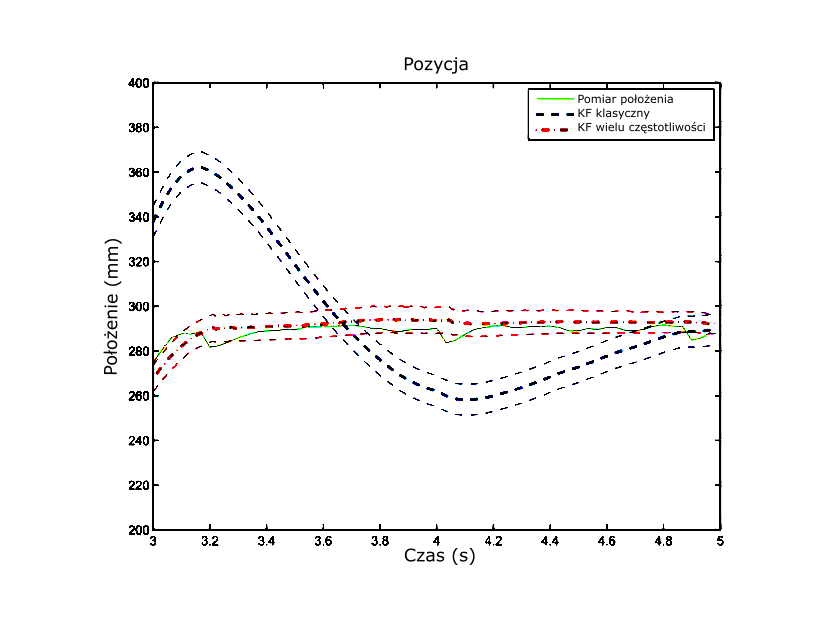
\includegraphics[width=0.95\textwidth]{images/Fig03.png}	
		\caption[Szacowanie położenia stawu z~użyciem klasycznego filtra Kalmana i~filtru Kalmana dostosowanego do różnych częstotliwości]{Szacowanie położenia stawu z~użyciem klasycznego filtra Kalmana (niebieski) i~filtru Kalmana dostosowanego do różnych częstotliwości (czerwony) \cite{Murray-Smith2014}}
		\label{fig:literature:feng}
	\end{figure}
\end{savenotes}
																																																			
Na podstawie wykresów zamieszczonych w~artykule Fanga i~Murray-Smitha można oszacować, że zaproponowana przez nich metoda określa pozycję stawów z~dokładnością $1.5 cm$ -- $2 cm$. Opublikowane diagramy pokazują jedynie wykresy wygenerowane przez zaledwie $5s$, więc problematyczne staje się oszacowanie jak zachowa się ta metoda w~dłuższym okresie. Widać także, że metoda wykorzystująca modyfikację filtru Kalmana i uwzględniającą zróżnicowanie częstotliwości łączonych sygnałów, szybciej reaguje na zmiany w~wykonywanym ruchu, niż metoda oparta o~klasyczną implementację filtru Kalmana (ma mniejszą bezwładność).																																																	
W 2013 roku Helten i in. \cite{Helten2013} zaproponował połączenie ze sobą sygnałów z~IMU oraz mapy głębi wyznaczonej przez kontroler Kinect. Dane uzyskane z~obu źródeł pozwalają na zbudowanie mapy widoczności poszczególnych części ciała. Informacje zawarte w~tej mapie pozwalają z~kolei wygenerować model ciała odzwierciedlający pozę, w~jakiej znajduje się śledzona postać. Wygenerowanie modelu ciała śledzonej postaci pozwala na przeprowadzenie klasyfikacji tego modelu na podstawie wcześniej zdefiniowanego treningowego zbioru zawierającego modele ciała w~określonych, nazwanych pozach. Istotną cechą metody polegającej na klasyfikacji pozy, w~jakiej znajduje się śledzona postać był brak możliwości określenia położenia poszczególnych stawów, a~jedynie monitorowanie aktualnej aktywności śledzonej postaci. Dzięki temu można było określić czy dana osoba stoi, chodzi, czy siedzi, a~to z~kolei zapewniło, że metoda zaproponowana przez zespół Thomasa Heltena mogła być z~powodzeniem zastosowana w~systemach nadzorujących np. zachowanie osób starszych. W~związku z~tym metoda ta nie może być porównywana z~takimi metodami jak choćby opisana powyżej metoda zaproponowana przez Bo i in. \cite{Bo2011a}, natomiast autorzy porównali ją z~analogicznymi metodami rozpoznającymi pozy człowieka np. Ganapathi i in. \cite{Ganapathi2010} czy Baak i in. \cite{Baak2011}. Według opisu zamieszczonego w~omawianym artykule, autorzy wskazali, że uzyskane przez nich rezulataty prawidłowego rozponania póz oraz wyznaczenia na ich podstawie modelu szkieletowego było nie gorsze niż innych, podobnych metod opisanych w~literaturze dla wybranego zestawu 6 póz, wśród których były między innymi obroty czy kopnięcia. Jako miarę określającą dokładność dopasowania, zdefiniowano błąd wyznaczenia wybranych 16 stawów uproszczonego modelu szkieletowego, jaki udało się wyznaczyć na podstawie rozpoznanej pozy, względem modelu szkieletowego otrzymanego w~wyniku śledzenia póz optycznym systemem śledzenia ruchu z~markerami firmy PhaseSpace. Średni błąd wyznaczania stawów przez metodę proponowaną przez zespół Thomasa Heltena wyniósł około $75mm$, co stanowiło poprawę o~blisko $50\%$ względem metody o~największym średnim błędzie pośród metod porównywanych w~omawianym artykule.																																																			
Ostatnią z~przytoczonych metod, ujętych w~literaturze i~dyskutowanych w~niniejszej pracy jest metoda zaproponowana w~artykule Kalkbrenner i in. \cite{Kalkbrenner2014}. Autorzy w~swojej metodzie wykorzystali dwa filtry łączące dane uzyskane za pomocą kontrolera Kinect oraz urządzeń pomiarowych opartych o~czujniki inercyjne. Pierwszym z~nich jest filtr zaproponowany przez Sebastiana Madgwicka \cite{Kalkbrenner2014}, drugim -- liniowy filtr Kalmana. Filtr Madgwicka\footnote{Opis filtru można znaleźć w~dodatku \ref{chap:appx:filters}.} pozwala na wyznaczanie orientacji urządzeń pomiarowych w~dwóch osiach dla czujników inercyjnych: akcelerometru i~żyroskopu oraz w~trzech dla czujników inercyjnych wspartych przez magentometr. Implementacja filtru przygotowana przez jego twórcę operowała na kwaternionach, co jest niewątpliwym ułatwieniem dla dalszych przekształceń. Jest to o~tyle istotne, że metoda zaproponowana przez Kalkbrennera wymaga, na podstawie wyniku uzyskanego za pomocą filtru Madgwicka oraz modelu długości kości, wyznaczenia pozycji kolejnych stawów  w~analogiczny sposób, jaki ma miejsce przy budowaniu hierarchicznego modelu szkieletowego ciała człowieka. Po wyznaczeniu pozycji stawów (w przypadku dyskutowanego artykułu wyznaczane są jedynie stawy jednej ręki: barkowy, jako korzeń, łokciowy oraz nadgarstkowy) były one łączone z~analogicznymi pozycjami stawów otrzymanymi z~Kinecta za pomocą liniowego filtru Kalmana.																																																			
Warto tutaj dodać, że autorzy uzależnili wartość współczynnika Kalmana $K$ (ang. \emph{Kalman gain}) od wartości przemieszczenia stawów $\delta s$ w~modelu szkieletowym Kinecta. Jeśli przemieszczenie to pomiędzy kolejnymi pomiarami było zbyt duże, oznaczało to utratę śledzenia i~brak wiarygodności pomiarów, a~co za tym idzie obniżenie istotności tych danych w~trakcie łączenia. Jako graniczną wartość zbyt dużego przemieszczenia się stawu ($\delta s = [\delta s_x, \delta s_y, \delta s_z]$), po której następowało ponowne wyznaczenie współczynnika Kalmana, autorzy przyjeli wartość $15cm$. W~sytuacji kiedy przemieszczenie się stawu pomiędzy kolejnymi pomiarami przekroczyło tę wartość graniczną następowało ponowne wyznaczenie najpierw macierzy kowariancji kontrolera Kinect $R$, a~następnie współczynnika Kalmana $K$, który wykorzystywał tę macierz odpowiednio według wzorów \ref{eq:kalman:matrixR} i~\ref{eq:kalman:gain}.
																																																	
\begin{equation}
	R = 
	\begin{pmatrix}
		R_x & 0   & 0   \\
		0   & R_y & 0   \\
		0   & 0   & R_z 
	\end{pmatrix} +
	\begin{pmatrix}
		\delta s_x^2 & 0            & 0            \\
		0            & \delta s_y^2 & 0            \\
		0            & 0            & \delta s_z^2 
	\end{pmatrix} * \kappa
	\label{eq:kalman:matrixR}
\end{equation}
																																																			
\begin{equation}
	K = P * H^T * (H * P * H^T +R)^-1
	\label{eq:kalman:gain}
\end{equation}
gdzie:
\begin{conditions}
	H& macierz jednostkowa\\
	R& macierz kowariancji kontrolera Kinect\\
	P& macierz kowariancji czujników inercyjnych\\
	K& współczynnik Kalmana.
\end{conditions}
																																																			
Wartość współczynnika $\kappa$ we wzorze \ref{eq:kalman:matrixR} została przez autorów artukułu wyznaczona empirycznie na $15$.
																																																			
Twórcy omawianej metody podali wartość średniego odchylenia wyznaczania położenia wybranych stawów na $\pm 2.2cm$ wobec $\pm 5.5cm$ dla kontrolera Kinect pracującego samodzielnie. Z opisu zaproponowanej metody wynika, że dla wyznaczenia pozycji stawów na podstawie IMU, model długości poszczególnych kości pobrany był wprost z~danych Kinecta. Z jednej strony ułatwiło to późniejsze złączenie ze sobą pozycji stawów wyznaczonych przez Kinecta oraz wyznaczonych na podstawie pomiarów czujników inercyjnych, ponieważ jedyna różnica pomiędzy rzeczonymi stawami wynika z~orientacji kości łączących śledzone stawy. Z drugiej zaś strony, oszacowanie długości kości przez kontroler Kinect jest niedokładne i~zmienia się niemal w~każdej klatce pomiarowej, więc unimożliwiało to wyznaczenie prawdziwego modelu szkieletowego, w~którym długości poszczególnych kości odpowiadałyby prawdziwym długościom.
				
Na tej podstawie zasadnym wydaje się wprowadzenie modelu szkieletowego, którego długości poszczególnych kości miałyby stałe wartości. Wymagałoby to jednak wcześniejszego dokonania pomiarów poszczególnych kości w~celu zbudowania takiego modelu. Eliminując zaszumienie ostatecznych wyników przez zmienność długości kości, łączenie danych z~urządzenia Kinect i~czujników inercyjnych powinno odbywać się z~wykorzystaniem informacji o~tym, w~jakiej orientacji znajdują się poszczególne kości. Estymacja taka dostępna jest wśród danych udostępnianych przez oprogramowanie kontrolera Kinect, a~także jest dostępne w~wyniku działania urządzeń pomiarowych opartych o~czujniki inercyjne. Następnie wykorzystanie informacji o~obrotach, z~przygotowanym wcześniej modelem szkieletowym, pozwala wyznaczyć położenie poszczególnych stawów. Można przypuszczać, że wprowadzenie modelu szkieletowego o~stałych długościach kości i~wykorzystanie informacji o~ich obrocie da większą dokładność wyznaczania pozycji stawów niż bezpośrednie łączenie ze sobą pozycji stawów wyznaczonych w~dwóch modelach szkieltowych, dla każdego z~urządzeń pomiarowych mających zmienne długości kości. Powyższe spostrzeżenia stanowią podstawową przesłankę budowy nowej, auroskiej hybrydowej metody śledzenia ruchu kończyn.